%
% Copyright (C) 2018 Bruno Félix Rezende Ribeiro <oitofelix@ufu.br>
%
% Copying and distribution of this file, with or without modification,
% are permitted in any medium without royalty provided the copyright
% notice and this notice are preserved.  This file is offered as-is,
% without any warranty.
%

\documentclass[12pt,a4paper]{report}


%%%%%%%%%%%%%%%%%%%%%%%%%%%%%%%%%%%%%%%%%%%%%%%%%%%%%%%%%%%%%%%%%%%%%%%%
% Package imports
%%%%%%%%%%%%%%%%%%%%%%%%%%%%%%%%%%%%%%%%%%%%%%%%%%%%%%%%%%%%%%%%%%%%%%%%

\usepackage[utf8]{inputenc}
\usepackage[brazil]{babel}
\usepackage{amsmath}
\usepackage{amssymb}
\usepackage{amsthm}
\usepackage{mathtools}
\usepackage{changepage}
\usepackage{enumerate}
\usepackage{relsize}
\usepackage{hyperref}
\usepackage{listings}
\usepackage{color}
\usepackage{centernot}
\usepackage{inconsolata}
\usepackage[T1]{fontenc}
\usepackage[nottoc,numbib]{tocbibind}
\usepackage{parcolumns}


%%%%%%%%%%%%%%%%%%%%%%%%%%%%%%%%%%%%%%%%%%%%%%%%%%%%%%%%%%%%%%%%%%%%%%%%
% Listings package customization
%%%%%%%%%%%%%%%%%%%%%%%%%%%%%%%%%%%%%%%%%%%%%%%%%%%%%%%%%%%%%%%%%%%%%%%%

\definecolor{comment}{rgb}{0,0.6,0}
\definecolor{number}{rgb}{0.5,0.5,0.5}
\definecolor{string}{rgb}{0.58,0,0.82}
\definecolor{keyword}{rgb}{1,0,0}
\definecolor{background}{rgb}{1,1,1}
\definecolor{indent}{rgb}{0.8,0.8,0.8}
\newcommand{\kwd}[1]{\texttt{\textcolor{keyword}{#1}}}
\newcommand{\cmt}[1]{\texttt{\textcolor{comment}{#1}}}
\newcommand{\I}{\enspace\textcolor{indent}\vrule\hspace{2pt}}

\lstdefinestyle{mystyle}{
    backgroundcolor=\color{background},
    commentstyle=\color{comment},
    keywordstyle=\color{keyword},
    numberstyle=\tiny\color{number},
    stringstyle=\color{string},
    basicstyle=\footnotesize\ttfamily,
    breakatwhitespace=false,
    breaklines=true,
    captionpos=b,
    keepspaces=true,
    numbers=left,
    numbersep=5pt,
    showspaces=false,
    showstringspaces=false,
    showtabs=false,
    tabsize=2
}

\lstset{
  alsoletter={.},
  style=mystyle,
  lineskip={-0.3pt},
  mathescape=true,
  inputencoding=utf8,
  extendedchars=true,
  escapechar=!,
  framexleftmargin=3pt,
  framexrightmargin=3pt,
  framextopmargin=3pt,
  framexbottommargin=3pt,
  frame=tb, framerule=0pt,
  % escapeinside={(*}{*)},
  literate=
  {á}{{\'a}}1
  {à}{{\`a}}1
  {ã}{{\~a}}1
  {é}{{\'e}}1
  {ê}{{\^e}}1
  {í}{{\'i}}1
  {ó}{{\'o}}1
  {õ}{{\~o}}1
  {ö}{{\"o}}1
  {ú}{{\'u}}1
  {ü}{{\"u}}1
  {ç}{{\c{c}}}1
  {Á}{{\'A}}1
  {À}{{\`A}}1
  {Ã}{{\~A}}1
  {É}{{\'E}}1
  {Ê}{{\^E}}1
  {Í}{{\'I}}1
  {Ó}{{\'O}}1
  {Õ}{{\~O}}1
  {Ú}{{\'U}}1
  {Ü}{{\"U}}1
  {Ç}{{\c{C}}}1
}

\lstdefinelanguage{algorithm}{
  keywords = {ENTRADA,PARA,ENQUANTO,SE,E,RETORNE}
}

\lstdefinelanguage{userrpl}{
  keywords = {
    WHILE, REPEAT, HEAD, TAIL, STO, IF, NOT, AND, THEN,
    SAME, END, ELSE, OR, DUP, DOLIST, EVAL, TEVAL, NIP, SIZE, GET, FOR, NEXT, CASE,
    START, STEP, DO, UNTIL, DROP, PICK, ROLL, ROLLD, NOVAL, RAND, RND, DUPDUP,
    PUSH, HOME, POP, IFERR, RCL, SUMLIST, MAX, STREAM, STREAMLIST, SWAP,
    RCLPOLYORD, QUICKSORT, GETI, SF, CF, PLEX, UNROT, REVLIST, NEG, PREVLEX,
    RCLPOLYVX, OVER, NDUPN, PAIRLIST, RCLVX, STOVX, LNAME, TYPE, AXL, POS, DEGREE,
    PRODLIST, FDISTRIB, SREPL, LTERM, PUT, MONOMIALS, FXND, UNPAIRLIST,
    LCM, GCD, ABS, LCOEF, SIGN, POLYEQ, DOLISTX, POSPOLY, SPOLY, POSPOLYPAIR,
    PDIVORDER, PDIV, LMONO, STOPOLYVX, PGRLEX, STOPOLYORD, BUCHBERGER, SOLVE
  },
  comment=[l]{@}
}

\newcommand{\IF}{\kwd{IF}}   % IF
\newcommand{\THEN}{\kwd{THEN}}   % THEN
\newcommand{\ELSE}{\kwd{ELSE}}   % ELSE
\newcommand{\END}{\kwd{END}}   % END
\newcommand{\CASE}{\kwd{CASE}}   % CASE
\newcommand{\NEXT}{\kwd{NEXT}}   % NEXT
\newcommand{\STEP}{\kwd{STEP}}   % STEP
\newcommand{\DUP}{\kwd{DUP}}   % DUP
\newcommand{\SWAP}{\kwd{SWAP}}   % SWAP
\newcommand{\DROP}{\kwd{DROP}}   % DROP
\newcommand{\OVER}{\kwd{OVER}}   % OVER
\newcommand{\ROT}{\kwd{ROT}}   % ROT
\newcommand{\UNROT}{\kwd{UNROT}}   % UNROT
\newcommand{\ROLL}{\kwd{ROLL}}   % ROLL
\newcommand{\ROLLD}{\kwd{ROLLD}}   % ROLLD
\newcommand{\PICK}{\kwd{PICK}}   % PICK
\newcommand{\DUPN}{\kwd{DUPN}}   % DUPN
\newcommand{\UNPICK}{\kwd{UNPICK}}   % UNPICK
\newcommand{\DEPTH}{\kwd{DEPTH}}   % DEPTH
\newcommand{\DUPDUP}{\kwd{DUPDUP}}   % DUPDUP
\newcommand{\DROPN}{\kwd{DROPN}}   % DROPN
\newcommand{\NIP}{\kwd{NIP}}   % NIP
\newcommand{\NDUPN}{\kwd{NDUPN}}   % NDUPN

\newcommand{\DROPTWO}{\kwd{DROP2}}   % DROP2
\newcommand{\PICKTHREE}{\kwd{PICK3}}   % PICK3
\newcommand{\DUPTWO}{\kwd{DUP2}}   % DUP2

\newcommand{\NOT}{\kwd{NOT}}   % NOT
\newcommand{\AND}{\kwd{AND}}   % AND
\newcommand{\OR}{\kwd{OR}}   % OR
\newcommand{\XOR}{\kwd{XOR}}   % XOR

\newcommand{\SAME}{\kwd{SAME}}   % SAME
\newcommand{\EQEQ}{\kwd{==}}   % ==
\newcommand{\LESS}{\kwd{$<$}}   % <
\newcommand{\LEQ}{\kwd{$\leq$}}   % <=
\newcommand{\GREATER}{\kwd{$>$}}   % >
\newcommand{\GEQ}{\kwd{$\geq$}}   % >=
\newcommand{\DIFF}{\kwd{$\neq$}} % !=

\newcommand{\NEG}{\kwd{NEG}}   % NEG
\newcommand{\PLUS}{\kwd{+}}   % +
\newcommand{\MINUS}{\kwd{-}}   % -
\newcommand{\MUL}{\kwd{*}}   % *
\newcommand{\DIV}{\kwd{/}}   % /
\newcommand{\POWER}{\kwd{\^{}}}   % ^
\newcommand{\RAND}{\kwd{RAND}}   % RAND
\newcommand{\RND}{\kwd{RND}}   % RND
\newcommand{\MAX}{\kwd{MAX}}   % MAX
\newcommand{\LCM}{\kwd{LCM}}   % LCM
\newcommand{\GCD}{\kwd{GCD}}   % GCD
\newcommand{\ABS}{\kwd{ABS}}   % ABS
\newcommand{\SIGN}{\kwd{SIGN}}   % SIGN

\newcommand{\PUSH}{\kwd{PUSH}}   % PUSH
\newcommand{\POP}{\kwd{POP}}   % POP
\newcommand{\HOME}{\kwd{HOME}}   % HOME
\newcommand{\EVAL}{\kwd{EVAL}}   % EVAL
\newcommand{\TEVAL}{\kwd{TEVAL}}   % TEVAL
\newcommand{\NOVAL}{\kwd{NOVAL}}   % NOVAL
\newcommand{\TYPE}{\kwd{TYPE}}   % TYPE

\newcommand{\TOSTR}{\kwd{$\rightarrow$STR}}   % ->STR
\newcommand{\STRTO}{\kwd{STR$\rightarrow$}}   % STR->
\newcommand{\SREPL}{\kwd{SREPL}}   % SREPL

\newcommand{\PIPE}{\kwd{|}}   % |
\newcommand{\LNAME}{\kwd{LNAME}}   % LNAME
\newcommand{\FXND}{\kwd{FXND}}   % FXND
\newcommand{\DEGREE}{\kwd{DEGREE}}   % DEGREE
\newcommand{\FDISTRIB}{\kwd{FDISTRIB}}   % FDISTRIB

\newcommand{\STO}{\kwd{STO}} % STO
\newcommand{\STOPLUS}{\kwd{STO+}} % STO+
\newcommand{\STOMINUS}{\kwd{STO-}} % STO-
\newcommand{\RCL}{\kwd{RCL}} % RCL
\newcommand{\RCLVX}{\kwd{RCLVX}} % RCLVX
\newcommand{\STOVX}{\kwd{STOVX}} % STOVX

\newcommand{\SF}{\kwd{SF}} % SF
\newcommand{\CF}{\kwd{CF}} % CF
\newcommand{\FSQ}{\kwd{FS?}} % FS?
\newcommand{\FCQ}{\kwd{FC?}} % FC?

\newcommand{\POS}{\kwd{POS}}   % POS
\newcommand{\AXL}{\kwd{AXL}}   % AXL
\newcommand{\REVLIST}{\kwd{REVLIST}}   % REVLIST
\newcommand{\TOLIST}{\kwd{$\rightarrow$LIST}} % ->LIST
\newcommand{\TAIL}{\kwd{TAIL}} % TAIL
\newcommand{\SIZE}{\kwd{SIZE}} % SIZE
\newcommand{\SIGMALIST}{\kwd{$\Sigma$LIST}}   % ΣLIST
\newcommand{\PILIST}{\kwd{$\Pi$LIST}}   % ΠLIST
\newcommand{\DOLIST}{\kwd{DOLIST}} % DOLIST
\newcommand{\STREAM}{\kwd{STREAM}} % STREAM
\newcommand{\GET}{\kwd{GET}} % GET
\newcommand{\GETI}{\kwd{GETI}} % GETI
\newcommand{\PUT}{\kwd{PUT}} % PUT
\newcommand{\SOLVE}{\kwd{SOLVE}} % SOLVE

\newcommand{\SINSERTSORTSTACK}{\kwd{\$INSERTSORTSTACK}}   % $INSERTSORTSTACK
\newcommand{\SQUICKSORTSTACK}{\kwd{\$QUICKSORTSTACK}}   % $QUICKSORTSTACK
\newcommand{\QUICKSORT}{\kwd{QUICKSORT}}   % QUICKSORT
\newcommand{\SUMLIST}{\kwd{SUMLIST}}   % SUMLIST
\newcommand{\PRODLIST}{\kwd{PRODLIST}}   % PRODLIST
\newcommand{\STREAMLIST}{\kwd{STREAMLIST}}   % STREAMLIST
\newcommand{\PAIRLIST}{\kwd{PAIRLIST}}   % PAIRLIST
\newcommand{\UNPAIRLIST}{\kwd{UNPAIRLIST}}   % UNPAIRLIST
\newcommand{\DOLISTX}{\kwd{DOLISTX}}   % DOLISTX

\newcommand{\STOPOLYVX}{\kwd{STOPOLYVX}}   % STOPOLYVX
\newcommand{\RCLPOLYVX}{\kwd{RCLPOLYVX}}   % RCLPOLYVX
\newcommand{\STOPOLYORD}{\kwd{STOPOLYORD}}   % STOPOLYORD
\newcommand{\RCLPOLYORD}{\kwd{RCLPOLYORD}}   % RCLPOLYORD
\newcommand{\PLEX}{\kwd{PLEX}}   % PLEX
\newcommand{\PREVLEX}{\kwd{PREVLEX}}   % PREVLEX
\newcommand{\PGRLEX}{\kwd{PGRLEX}}   % PGRLEX
\newcommand{\PGREVLEX}{\kwd{PGREVLEX}}   % PGREVLEX
\newcommand{\TDEG}{\kwd{TDEG}}   % TDEG
\newcommand{\MDEG}{\kwd{MDEG}}   % MDEG
\newcommand{\LCOEF}{\kwd{LCOEF}}   % LCOEF
\newcommand{\LMONO}{\kwd{LMONO}}   % LMONO
\newcommand{\LTERM}{\kwd{LTERM}}   % LTERM
\newcommand{\SPOLYTOLIST}{\kwd{\$POLY{$\rightarrow$}LIST}}   % $POLY->LIST
\newcommand{\SLISTTOPOLY}{\kwd{\$LIST{$\rightarrow$}POLY}}   % $LIST->POLY
\newcommand{\SLISTTOMONO}{\kwd{\$LIST{$\rightarrow$}MONO}}   % $LIST->MONO
\newcommand{\SMONOTOLIST}{\kwd{\$MONO{$\rightarrow$}LIST}}   % $MONO->LIST
\newcommand{\PORDER}{\kwd{PORDER}}   % PORDER
\newcommand{\SPORDER}{\kwd{\$PORDER}}   % $PORDER
\newcommand{\SCOEF}{\kwd{\$COEF}}   % $COEF
\newcommand{\SMONODIV}{\kwd{\$MONODIV}}   % $MONODIV
\newcommand{\MONOMIALS}{\kwd{MONOMIALS}}   % MONOMIALS
\newcommand{\PDIV}{\kwd{PDIV}}   % PDIV
\newcommand{\SMONOLCM}{\kwd{\$MONOLCM}}   % $MONOLCM
\newcommand{\SPOLY}{\kwd{SPOLY}}   % SPOLY
\newcommand{\SPOLYINT}{\kwd{\$POLYINT}}   % $POLYINT
\newcommand{\POLYEQ}{\kwd{POLYEQ}}   % POLYEQ
\newcommand{\POSPOLY}{\kwd{POSPOLY}}   % POSPOLY
\newcommand{\POSPOLYPAIR}{\kwd{POSPOLYPAIR}}   % POSPOLYPAIR

\newcommand{\BUCHBERGER}{\kwd{BUCHBERGER}}   % BUCHBERGER
\newcommand{\SReduceAll}{\kwd{\$ReduceAll}}   % $ReduceAll
\newcommand{\SNewBasis}{\kwd{\$NewBasis}}   % $NewBasis
\newcommand{\SNormalForm}{\kwd{\$NormalForm}}   % $NormalForm
\newcommand{\SCriterionOne}{\kwd{\$Criterion1}}   % $Criterion1
\newcommand{\SCriterionTwo}{\kwd{\$Criterion2}}   % $Criterion2
\newcommand{\PDIVORDER}{\kwd{PDIVORDER}}   % PDIVORDER
\newcommand{\SSelStrategy}{\kwd{\$SelStrategy}}   % $SelStrategy

\newcommand{\OP}{\kwd{$\ll$}}   % <<
\newcommand{\CP}{\kwd{$\gg$}}   % >>
\newcommand{\TO}{\kwd{$\rightarrow$}} % ->
\newcommand{\FROM}{\kwd{$\leftarrow$}} % <-


%%%%%%%%%%%%%%%%%%%%%%%%%%%%%%%%%%%%%%%%%%%%%%%%%%%%%%%%%%%%%%%%%%%%%%%%
% Document metric
%%%%%%%%%%%%%%%%%%%%%%%%%%%%%%%%%%%%%%%%%%%%%%%%%%%%%%%%%%%%%%%%%%%%%%%%

\setlength{\textwidth}{17cm}
\setlength{\textheight}{24cm}
\setlength{\evensidemargin}{0cm}
\setlength{\oddsidemargin}{-0.5cm}
\setlength{\topmargin}{-2cm}
\renewcommand{\baselinestretch}{1.5}


%%%%%%%%%%%%%%%%%%%%%%%%%%%%%%%%%%%%%%%%%%%%%%%%%%%%%%%%%%%%%%%%%%%%%%%%
% New commands
%%%%%%%%%%%%%%%%%%%%%%%%%%%%%%%%%%%%%%%%%%%%%%%%%%%%%%%%%%%%%%%%%%%%%%%%

\newcommand{\N}{\mathbb{N}}
\newcommand{\Z}{\mathbb{Z}}
\newcommand{\Q}{\mathbb{Q}}
\newcommand{\R}{\mathbb{R}}
\newcommand{\C}{\mathbb{C}}

\newcommand{\lee}{\enspace\land\enspace}
\newcommand{\lou}{\enspace\lor\enspace}
\newcommand{\lequiv}{\enspace\Longleftrightarrow\enspace}

\newcommand{\function}[3]{{#1:#2\rightarrow#3}}
\newcommand{\suchthat}{\enspace\middle|\enspace}
\newcommand{\divides}{\parallel}
\newcommand{\ndivides}{\nparallel}
\newcommand{\boxedLeftArrow}{\raisebox{2pt}[\height][0pt]{
    \framebox{\raisebox{-1pt}[\height][0pt]{\(\Leftarrow\)}}}\enspace}
\newcommand{\boxedRightArrow}{\raisebox{2pt}[\height][0pt]{
    \framebox{\raisebox{-1pt}[\height][0pt]{\(\Rightarrow\)}}}\enspace}
\newcommand{\comment}[2]{\stackrel{\mathclap{\textnormal{\tiny\mbox{#2}}}}{#1}}

\newcommand{\crlf}{\mbox{}\\*}

\newcommand{\MyLine}{\hfill\noindent\rule[0.5ex]{\linewidth}{0.5pt}\\}
\newcommand{\SignatureLine}{
  \underline{\ \ \ \ \ \ \ \ \ \ \ \ \ \ \ \ \ \ \ \ \ \ \ \ \ \ \ \
    \ \ \ \ \ \ \ \ \ \ \ \ \ \ \ \ \ \ \ \ \ \ \ \ \ \ \ \ \ \ \ \ \
    \ \ \ \ \ \ \ \ \ \ \ \ \ \ \ \ \ \ \ \ }\\
}


%%%%%%%%%%%%%%%%%%%%%%%%%%%%%%%%%%%%%%%%%%%%%%%%%%%%%%%%%%%%%%%%%%%%%%%%
% New theorem environments
%%%%%%%%%%%%%%%%%%%%%%%%%%%%%%%%%%%%%%%%%%%%%%%%%%%%%%%%%%%%%%%%%%%%%%%%

\newtheorem{theorem}{Teorema}
\newtheorem{proposition}[theorem]{Proposição}
\newtheorem{definition}[theorem]{Definição}
\newtheorem{lemma}[theorem]{Lema}
\newtheorem{corollary}[theorem]{Corolário}
\newtheorem{example}[theorem]{Exemplo}
\newtheorem*{notation}{Notação}
\numberwithin{theorem}{chapter}


%%%%%%%%%%%%%%%%%%%%%%%%%%%%%%%%%%%%%%%%%%%%%%%%%%%%%%%%%%%%%%%%%%%%%%%%
% New math operators
%%%%%%%%%%%%%%%%%%%%%%%%%%%%%%%%%%%%%%%%%%%%%%%%%%%%%%%%%%%%%%%%%%%%%%%%

\DeclareMathOperator{\grau}{grau}
\DeclareMathOperator{\multigrau}{multigrau}
\DeclareMathOperator{\CL}{CL}
\DeclareMathOperator{\ML}{ML}
\DeclareMathOperator{\TL}{TL}
\DeclareMathOperator{\mmc}{mmc}
\DeclareMathOperator{\Sp}{S}
\DeclareMathOperator{\Reduza}{Reduza}
\DeclareMathOperator{\NovaBase}{NovaBase}
\DeclareMathOperator{\MenorMMC}{MenorMMC}
\DeclareMathOperator{\CriterioUm}{Crit\acute{e}rio1}
\DeclareMathOperator{\CriterioDois}{Crit\acute{e}rio2}
\DeclareMathOperator{\FormaNormal}{FormaNormal}
\DeclareMathOperator{\Escolha}{Escolha}
\DeclareMathOperator{\Buchberger}{Buchberger}
\DeclareMathOperator{\Divisao}{Divis\tilde{a}o}



%%%%%%%%%%%%%%%%%%%%%%%%%%%%%%%%%%%%%%%%%%%%%%%%%%%%%%%%%%%%%%%%%%%%%%%%
% Common text macros
%%%%%%%%%%%%%%%%%%%%%%%%%%%%%%%%%%%%%%%%%%%%%%%%%%%%%%%%%%%%%%%%%%%%%%%%

\newcommand{\WorkTitle}{Estudo e Implementação do Algoritmo de
  Buchberger na linguagem UserRPL para a Calculadora Gráfica HP 50g}
\newcommand{\WorkDescription}{Monografia apresentada à Faculdade de
  Matemática da Universidade Federal de Uberlândia como requisito
  parcial para obtenção do título de Bacharel em Matemática, sob a
  orientação do Prof. Dr. Victor Gonzalo Lopez Neumann.}
\newcommand{\WorkAuthor}{Bruno Félix Rezende Ribeiro}
\newcommand{\WorkLocal}{Uberlândia - MG} \newcommand{\WorkYear}{2018}


%%%%%%%%%%%%%%%%%%%%%%%%%%%%%%%%%%%%%%%%%%%%%%%%%%%%%%%%%%%%%%%%%%%%%%%%
%  Outer title page
%%%%%%%%%%%%%%%%%%%%%%%%%%%%%%%%%%%%%%%%%%%%%%%%%%%%%%%%%%%%%%%%%%%%%%%%

\begin{document}

\begin{center}
  \MyLine
  {\LARGE\textbf{Universidade Federal de Uberlândia}}\\
  {\Large Faculdade de Matemática}
  \MyLine
\end{center}

\vspace{1cm}

\begin{center}
  {\LARGE\WorkAuthor}
\end{center}

\vspace{\fill}

\begin{center}
  {\LARGE\textbf{\WorkTitle}}
\end{center}

\vspace{\fill}

\begin{center}
  \textbf{\WorkLocal}\\
  \textbf{\WorkYear}
\end{center}

\thispagestyle{empty}


%%%%%%%%%%%%%%%%%%%%%%%%%%%%%%%%%%%%%%%%%%%%%%%%%%%%%%%%%%%%%%%%%%%%%%%%
% Inner title page
%%%%%%%%%%%%%%%%%%%%%%%%%%%%%%%%%%%%%%%%%%%%%%%%%%%%%%%%%%%%%%%%%%%%%%%%

\newpage

\begin{center}
  {\LARGE\WorkAuthor}
\end{center}

\vspace{\fill}

\begin{center}
  {\LARGE\textbf{\WorkTitle}}
\end{center}

\vspace{1cm}

\begin{adjustwidth}{7cm}{0cm}
  {\large\WorkDescription}
\end{adjustwidth}

\vspace{\fill}

\begin{center}
  \textbf{\WorkLocal}\\
  \textbf{\WorkYear}
\end{center}

\thispagestyle{empty}


%%%%%%%%%%%%%%%%%%%%%%%%%%%%%%%%%%%%%%%%%%%%%%%%%%%%%%%%%%%%%%%%%%%%%%%%
% Signature page
%%%%%%%%%%%%%%%%%%%%%%%%%%%%%%%%%%%%%%%%%%%%%%%%%%%%%%%%%%%%%%%%%%%%%%%%

\newpage

\begin{center}
  {\LARGE\WorkAuthor}
\end{center}

\vspace{1cm}

\begin{center}
  {\LARGE\textbf{\WorkTitle}}
\end{center}

\vspace{\fill}

\begin{adjustwidth}{7cm}{0cm}
  {\large\WorkDescription}
\end{adjustwidth}

\vspace{\fill}

\begin{center}
  {\large Aprovada em 13/12/2018}

  \vspace{\fill}

  {\large\textbf{BANCA EXAMINADORA}}

  \vspace{2em}\centerline{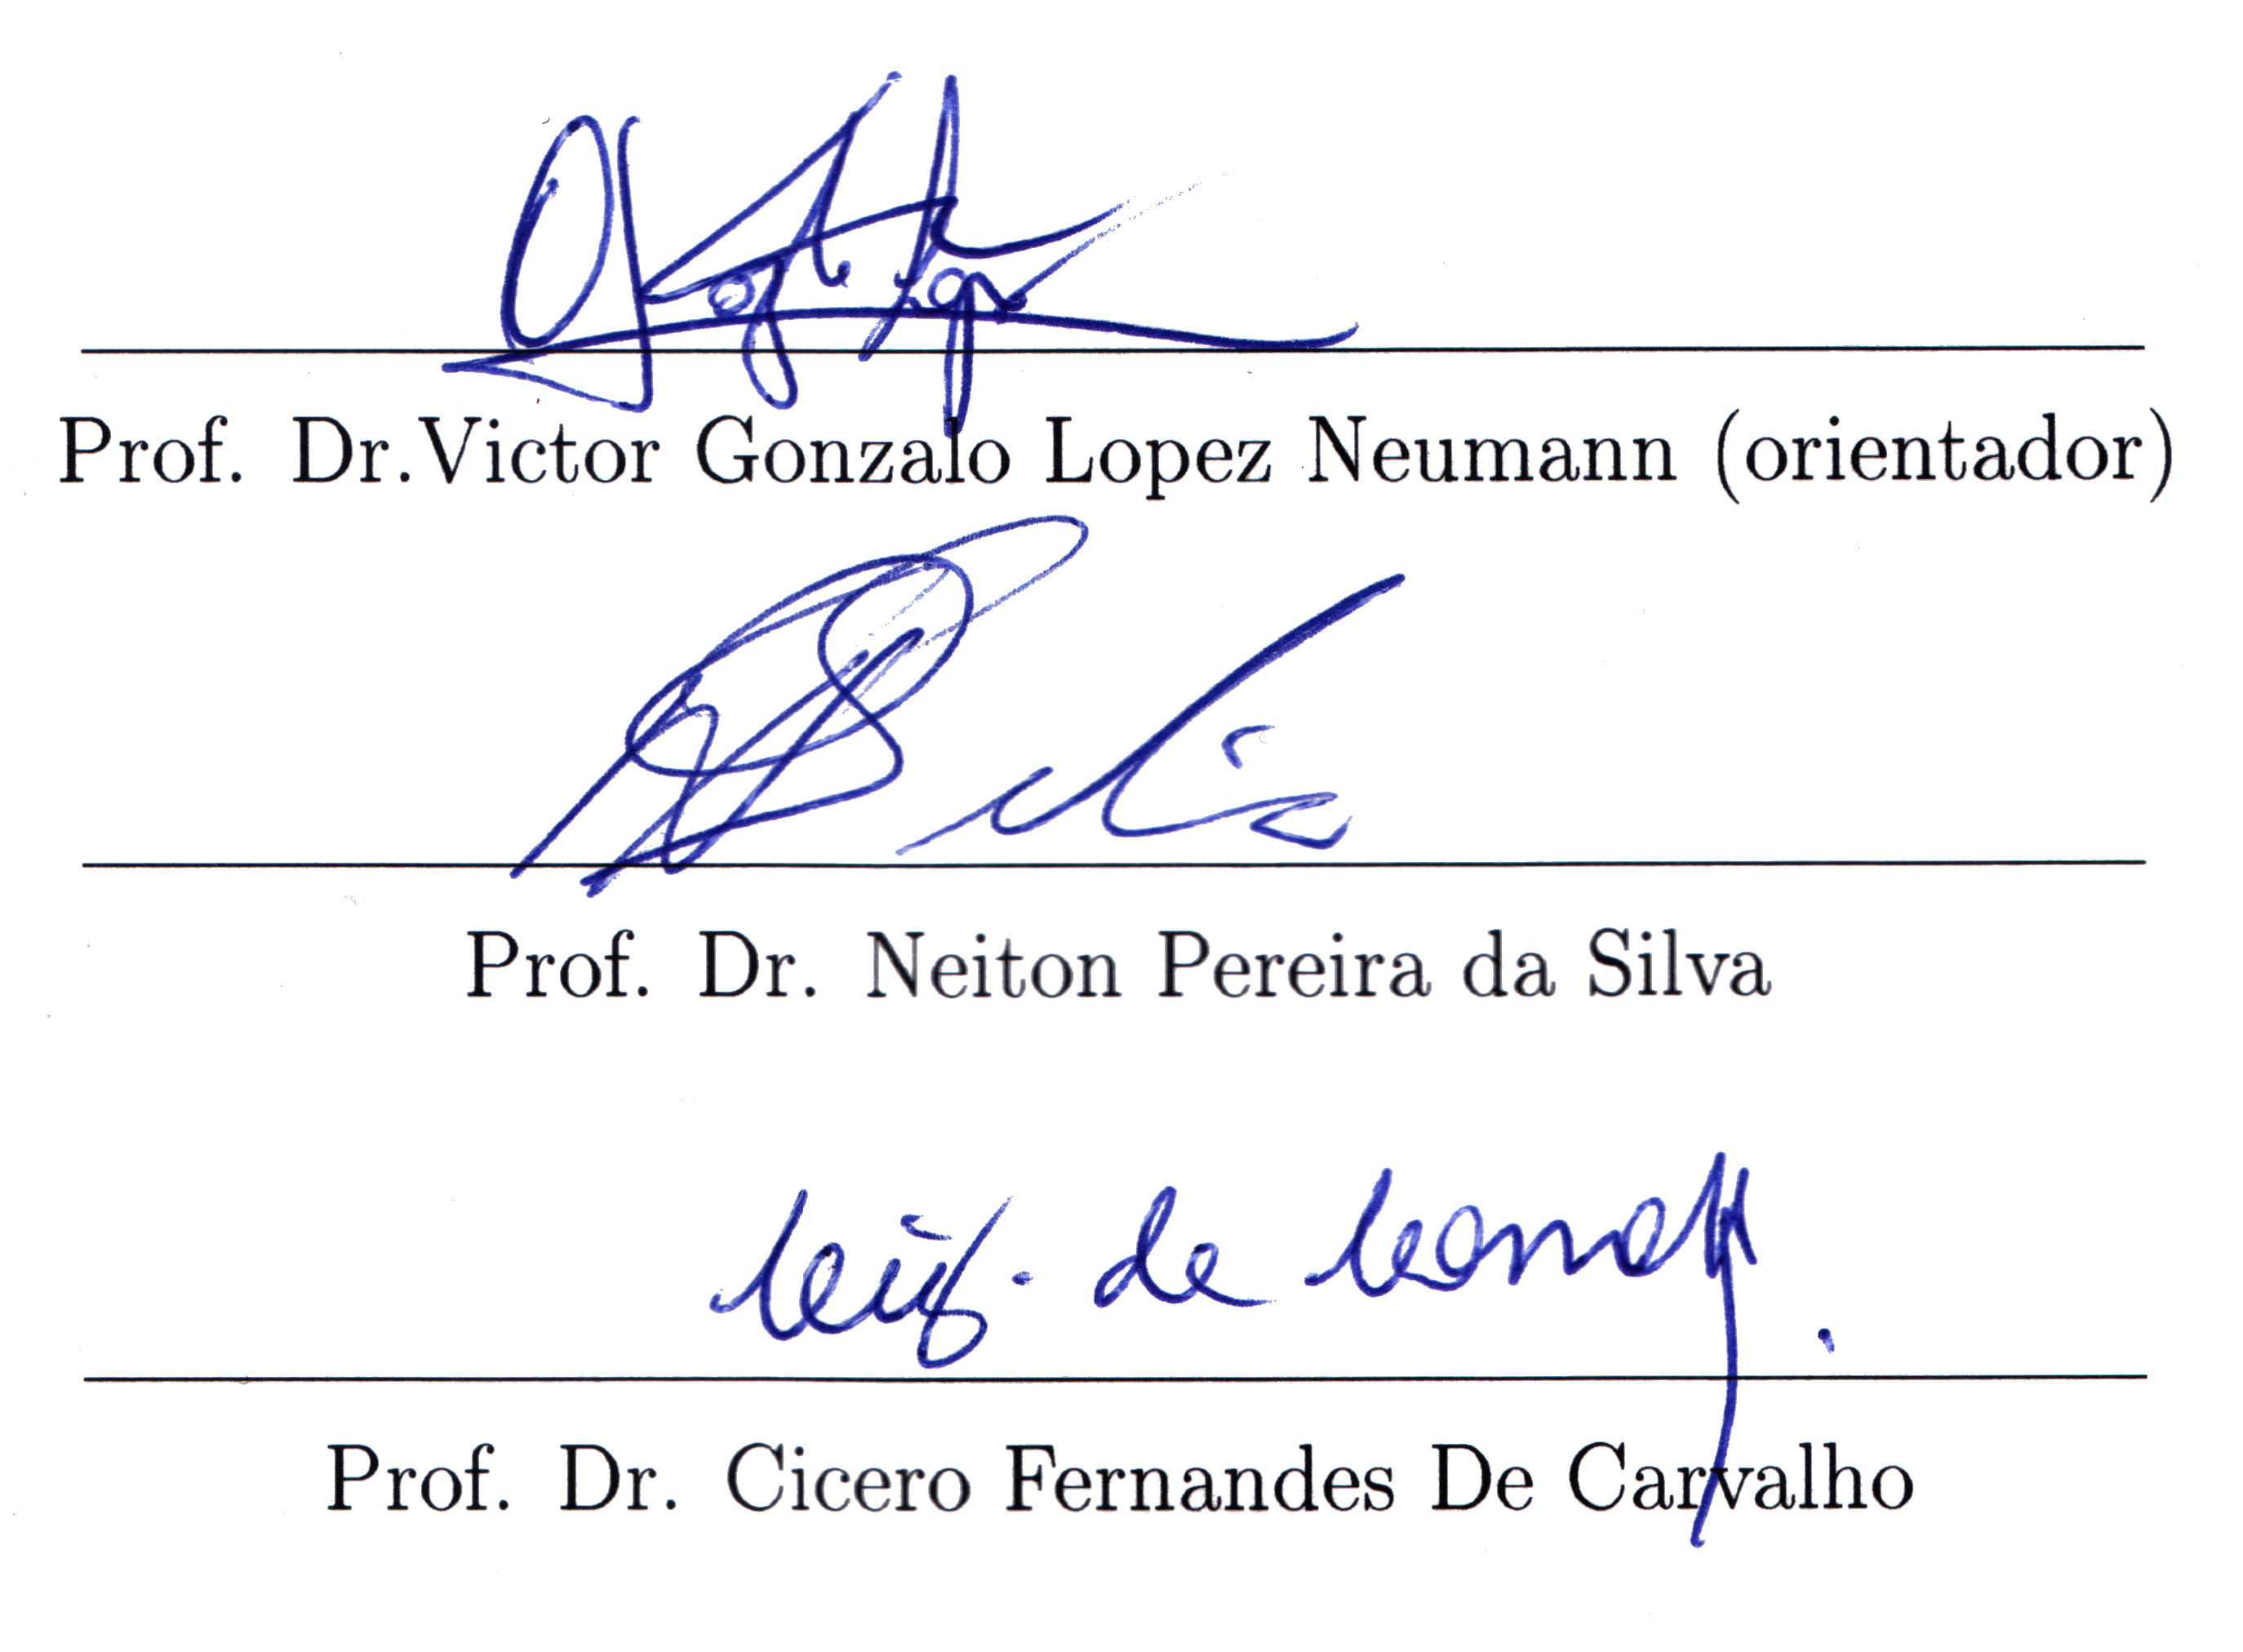
\includegraphics[scale=1]{sig}}\vspace{2em}


  %% \vspace{1.5cm}

  %% \SignatureLine
  %% {\large Prof. Dr.Victor Gonzalo Lopez Neumann (orientador)}

  %% \vspace{\fill}

  %% \SignatureLine
  %% {\large Prof. Dr. Neiton Pereira da Silva}

  %% \vspace{\fill}

  %% \SignatureLine
  %% {\large Prof. Dr. Cicero Fernandes De Carvalho}
\end{center}

\thispagestyle{empty}


%%%%%%%%%%%%%%%%%%%%%%%%%%%%%%%%%%%%%%%%%%%%%%%%%%%%%%%%%%%%%%%%%%%%%%%%
% Acknowledgements page
%%%%%%%%%%%%%%%%%%%%%%%%%%%%%%%%%%%%%%%%%%%%%%%%%%%%%%%%%%%%%%%%%%%%%%%%

\newpage

\chapter*{Agradecimentos}

\noindent

Agradeço a todos os matemáticos que fundamentaram as teorias sobre as
quais o presente trabalho se baseia, em particular Bruno Buchberger
pelo brilhantismo de sua inovação matemática teórica e computacional.

Agradeço aos engenheiros da Hewlett Packard responsáveis pelo
desenvolvimento da série de calculadoras baseadas na linguagem
UserRPL, cuja destreza técnica possibilitou tanto divertimento na
programação do modelo 50g.

Agradeço a todos os professores que me ensinaram as habilidades
necessárias para a produção do presente trabalho, em particular meu
orientador Victor Neumann por sua grande competência em álgebra
comutativa e generoso apoio frente às dificuldades.

Agradeço a todos os entes queridos que me deram suporte emocional para
a conclusão deste trabalho, em particular minha futura esposa Maiane
Ribeiro pelo seu amor imensurável.

Por último, mas não menos importante, agradeço ao \(\varnothing\) por
tudo existir.

\thispagestyle{empty}


%%%%%%%%%%%%%%%%%%%%%%%%%%%%%%%%%%%%%%%%%%%%%%%%%%%%%%%%%%%%%%%%%%%%%%%%
% Summary page
%%%%%%%%%%%%%%%%%%%%%%%%%%%%%%%%%%%%%%%%%%%%%%%%%%%%%%%%%%%%%%%%%%%%%%%%

\newpage

\chapter*{Resumo}

Neste trabalho estuda-se os conceitos e resultados algébricos que
fundamentam a teoria das bases de Gröbner e o algoritmo de Buchberger
que possibilita o cálculo efetivo destas.  A teoria é estabelecida com
respeito a um anel polinomial em um número arbitrário de variáveis com
coeficientes sobre um corpo qualquer.  Dá-se ênfase aos assuntos
relativos à ordem monomial, algoritmo da divisão, ideais monomiais,
lema de Dickson e teorema da base de Hilbert.  A título de
curiosidade, desenvolve-se uma implementação do algoritmo de
Buchberger como descrito originalmente em [Buchberger, 1985] na
linguagem UserRPL para a Calculadora Gráfica HP 50g e explora-se suas
propriedades técnicas e computacionais.  Esta implementação provê
suporte para polinômios com coeficientes complexos em um número
arbitrário de variáveis com ordenações monomiais canônicas
pré-definidas e também programáveis pelo usuário.

\vspace{1cm}

\noindent{\bf Palavras-Chave:} Álgebra Computacional. Bases de
Gröbner. Algoritmo de Buchberger. UserRPL. HP 50g.

\thispagestyle{empty}


%%%%%%%%%%%%%%%%%%%%%%%%%%%%%%%%%%%%%%%%%%%%%%%%%%%%%%%%%%%%%%%%%%%%%%%%
% Table of contents
%%%%%%%%%%%%%%%%%%%%%%%%%%%%%%%%%%%%%%%%%%%%%%%%%%%%%%%%%%%%%%%%%%%%%%%%

\newpage

\tableofcontents

\thispagestyle{empty}


%%%%%%%%%%%%%%%%%%%%%%%%%%%%%%%%%%%%%%%%%%%%%%%%%%%%%%%%%%%%%%%%%%%%%%%%
% Introduction
%%%%%%%%%%%%%%%%%%%%%%%%%%%%%%%%%%%%%%%%%%%%%%%%%%%%%%%%%%%%%%%%%%%%%%%%

\chapter*{Introdução}
\addcontentsline{toc}{chapter}{Introdução}
\noindent

Dentro do ramo da álgebra comutativa e geometria algébrica
computacional uma \textit{base de Gröbner} é um tipo particular de
conjunto gerador de um ideal dentro de um anel polinomial sobre um
corpo qualquer.  O conceito de bases de Gröbner é fundamental para a
dedução de várias propriedades importantes de um ideal e sua variedade
algébrica associada, como dimensão e número de zeros.  O
\textit{algoritmo de Buchberger} permite o cálculo efetivo das bases
de Gröbner e é uma das principais ferramentas em sistemas algébricos
computacionais para a resolução de sistemas de equações polinomiais e
a computação de imagens de variedades algébricas sob projeções e
mapeamento racional.  Este algoritmo pode ser visto como uma
generalização multivariável não linear do algoritmo euclidiano para o
cálculo do máximo divisor comum de polinômios e da eliminação
gaussiana para sistemas lineares.  A teoria das bases de Gröbner,
junto com o algoritmo de Buchberger, foram introduzidas por Bruno
Buchberger em sua tese de doutorado, sendo o nome dado às bases
homenagem ao seu orientador Wolfgang Gröbner [Buchberger, 1985].

Na primeira parte deste trabalho estuda-se os conceitos e resultados
algébricos que fundamentam a teoria das bases de Gröbner e o algoritmo
de Buchberger que possibilita o cálculo efetivo destas.  A teoria é
estabelecida com respeito a um anel polinomial em um número arbitrário
de variáveis com coeficientes sobre um corpo qualquer.  Dá-se ênfase
aos assuntos relativos à ordem monomial, algoritmo da divisão, ideais
monomiais, lema de Dickson e teorema da base de Hilbert.  Na segunda
parte do presente trabalho desenvolve-se uma implementação do
algoritmo de Buchberger como descrito originalmente em [Buchberger,
1985] na linguagem UserRPL para a Calculadora Gráfica HP 50g e
explora-se suas propriedades técnicas e computacionais.



%%%%%%%%%%%%%%%%%%%%%%%%%%%%%%%%%%%%%%%%%%%%%%%%%%%%%%%%%%%%%%%%%%%%%%%%
% Chapter: Anéis, corpos e polinômios
%%%%%%%%%%%%%%%%%%%%%%%%%%%%%%%%%%%%%%%%%%%%%%%%%%%%%%%%%%%%%%%%%%%%%%%%

\chapter{Anéis, Corpos e Polinômios}

Neste capítulo revisaremos os conceitos pertinentes aos anéis, corpos
e polinômios que fundamentam a teoria estudada.

\begin{definition}[Anel comutativo]
  Sejam \(A\) um conjunto não-vazio, e as operações \(+\) e \(\cdot\)
  definidas sobre \(A\).  A terna \((A,+,\cdot)\) é um \textbf{anel
    comutativo} se satisfaz as seguintes propriedades:

  \begin{description}
  \item[(Associatividade)] Para todos \(a\), \(b\) e \(c\) em \(A\):
    \begin{itemize}
    \item \((a + b) + c = a + ( b + c)\)
    \item \((a \cdot b) \cdot c = a \cdot (b \cdot c)\)
    \end{itemize}

  \item[(Comutatividade)] Para todos \(a\) e \(b\) em \(A\):
    \begin{itemize}
    \item \(a + b = b + a\)
    \item \(a \cdot b = b \cdot a\)
    \end{itemize}

  \item[(Distributividade)] Para todos \(a\), \(b\) e \(c\) em \(A\):
    \begin{itemize}
    \item \(a \cdot (b + c) = a \cdot b + a \cdot c\)
    \end{itemize}

  \item[(Identidade)] Para todo \(a\) em \(A\), existem \(0\) e \(1\)
    em \(A\) tais que:
    \begin{itemize}
    \item \(a + 0 = a\)
    \item \(a \cdot 1 = a\)
    \end{itemize}

    \begin{samepage}
    \item[(Inverso aditivo)] Para todo \(a\) em \(A\), existe \(b\) em
      \(A\) tal que:
      \begin{itemize}
      \item \(a + b = 0\)
      \end{itemize}
    \end{samepage}
  \end{description}
\end{definition}

Quando as operações aditiva e multiplicativa estão subentendidas, não
ocorrendo risco de ambiguidade, identifica-se a terna \((A,+,\cdot)\)
com o próprio conjunto \(A\), chamando-se a este de ``anel''.

\begin{definition}[Corpo]
  Um anel comutativo \((A,+,\cdot)\) é um \textbf{corpo} se satisfaz a
  seguinte propriedade:
  \begin{description}
  \item[(Inverso multiplicativo)] Para todo \(a \neq 0\) em \(A\),
    existe \(b\) em \(A\) tal que:
    \begin{itemize}
    \item \(a \cdot b = 1\)
    \end{itemize}
  \end{description}
\end{definition}

Quando as operações aditiva e multiplicativa estão subentendidas, não
ocorrendo risco de ambiguidade, identifica-se a terna \((F,+,\cdot)\)
com o próprio conjunto \(F\), chamando-se a este de ``corpo''.

\begin{definition}[Monômio]
  Um \textbf{monômio} nas variáveis \(x_1,\ldots,x_n\) é uma expressão
  algébrica da forma \(\prod\limits_{i=1}^n{x_i^{\alpha_i}}\), onde
  \(\alpha_i \in \N\) para \(1 \leq i \leq n\).
\end{definition}

\begin{notation}
  Denota-se \(\prod\limits_{i=1}^n{x_i^{\alpha_i}}\) por \(x^\alpha\),
  onde \(x = (x_1,\ldots,x_n)\) e \(\alpha =
  (\alpha_1,\ldots,\alpha_n)\).
\end{notation}

\begin{definition}[Grau total de monômio]
  O \textbf{grau total de um monômio} \(f = x^\alpha\) é definido como
  \({\grau(f) \coloneqq \sum\limits_{i=1}^n{\alpha_i}}\).
\end{definition}

\begin{definition}[Polinômio]
  Um \textbf{polinômio} nas variáveis \(x_1,\ldots,x_n\) com
  coeficientes sobre um corpo \(F\) é uma expressão algébrica da forma
  \(\sum\limits_{\alpha \in A} a_{\alpha}x^\alpha\), onde \(A\) é um
  subconjunto finito de \(\N^n\), e \(a_{\alpha} \in F\) para todo
  \(\alpha \in A\).
\end{definition}

\begin{notation}\mbox{}
  \begin{itemize}
  \item Quando não há risco de ambiguidade nem necessidade de
    explicitação, costuma-se omitir o conjunto \(A\) na notação da
    expressão algébrica geral de um polinômio (como acima) por:
    \(\sum\limits_{\alpha} a_{\alpha}x^\alpha\);

  \item Denota-se o conjunto de todos os polinômios nas variáveis
    \(x_1,\ldots,x_n\) com coeficientes sobre um corpo \(F\) por
    \(F[x_1,\ldots,x_n]\);
  \end{itemize}
\end{notation}

\begin{definition}[Grau total de polinômio]
  O \textbf{grau total de um polinômio} \(f = \sum\limits_{\alpha}
  a_{\alpha}x^\alpha \neq 0\) é definido como \(\grau(f) \coloneqq
  \max\left\{\grau(x^\alpha) \suchthat a_{\alpha} \neq 0\right\}\).
\end{definition}

\begin{definition}[Ideal]
  Um subconjunto \(I \subset F[x_1,\ldots,x_n]\) é um \textbf{ideal}
  se satisfaz:
  \begin{enumerate}[(i)]
    \item \(0 \in I\);
    \item Se \(f, g \in I\), então \(f + g \in I\);
    \item Se \(f \in I\) e \(h \in F[x_1,\ldots,x_n]\), então \(h
      \cdot f \in I\);
  \end{enumerate}
\end{definition}

Note que o menor ideal possível, chamado de ``\textbf{ideal trivial}'', é
\(\{0\}\).

\begin{notation}
  Sejam \(f_1,\ldots,f_s\) polinômios em \(F[x_1,\ldots,x_n]\).
  Denota-se \[\langle f_1,\ldots,f_s \rangle \coloneqq \left\{
    \sum\limits_{i=1}^s{h_if_i} \suchthat h_1,\ldots,h_s \in
    F[x_1,\ldots,x_n]\right\}.\]
\end{notation}

\begin{lemma}[Ideal gerado]
  Se \(f_1,\ldots,f_s \in F[x_1,\ldots,x_n]\), então \(\langle
  f_1,\ldots,f_s \rangle\) é um ideal de \(F[x_1,\ldots,x_n]\), que
  chamamos de \textbf{ideal gerado} por \(f_1,\ldots,f_s\).
\end{lemma}

\begin{proof}
  Primeiramente, \(0 \in \langle f_1,\ldots,f_s \rangle\) visto que
  \(0 = \sum\limits_{i=1}^s{0 \cdot f_i}\).  Agora, suponha que \(f =
  \sum\limits_{i=1}^s{p_if_i}\) e \(g = \sum\limits_{i=1}^sq_if_i\), e seja
  \(h \in F[x_1,\ldots,x_n]\).  Então as equações,
  \begin{align*}
    f + g &= \sum_{i=1}^s (p_i + q_i)f_i\\
    hf &= \sum_{i=1}^s(hp_i)f_i
  \end{align*}
  completam a prova de que \(\langle f_1,\ldots,f_s \rangle\) é um
  ideal.
\end{proof}


%%%%%%%%%%%%%%%%%%%%%%%%%%%%%%%%%%%%%%%%%%%%%%%%%%%%%%%%%%%%%%%%%%%%%%%%
% Chapter: Ordem monomial e algoritmo da divisão
%%%%%%%%%%%%%%%%%%%%%%%%%%%%%%%%%%%%%%%%%%%%%%%%%%%%%%%%%%%%%%%%%%%%%%%%
\chapter{Ordem Monomial e Algoritmo da Divisão}

\begin{definition}[Relação]
  Uma \textbf{relação} sobre um conjunto \(M\) é um subconjunto de
  \(M^2 = M \times M\).
\end{definition}

\begin{notation}
  Denota-se \((f,g) \in \enspace\geq\) por \(f \geq g\).
\end{notation}

\begin{definition}[Ordem]
  \textbf{Ordem} sobre um conjunto \(M\) é uma relação \(\geq\) tal
  que para todo \(f\), \(g\) e \(h\) em \(M\) satisfaz:
  \begin{description}
  \item[(Reflexiva)] \(f \geq f\);
  \item[(Anti-simétrica)] Se \(f \geq g\) e \(g \geq f\), então \(f = g\);
  \item[(Transitiva)] Se \(f \geq g\) e \(g \geq h\), então \(f \geq h\);
  \end{description}
\end{definition}

\begin{notation}
  Denota-se:
  \begin{itemize}
  \item \(f \geq g\) por \(g \leq f\);
  \item \(f \geq g\) e \(f \neq g\) por \(f > g\);
  \item \(f > g\) por \(g < f\);
  \end{itemize}
\end{notation}

\begin{definition}[Ordem total]
  \textbf{Ordem total} é uma ordem \(\geq\) sobre um conjunto \(M\)
  tal que para todo \(f\) e \(g\) em \(M\) verifica-se exclusivamente
  um dos seguintes casos:
  \begin{itemize}
    \item \(f > g\);
    \item \(f = g\);
    \item \(f < g\);
  \end{itemize}
\end{definition}

A ordem usual dos números reais é uma ordem total, pois para quaisquer
dois elementos vale a tricotomia.

\begin{definition}[Boa ordem]
  \textbf{Boa ordem} é uma ordem \(\geq\) sobre um conjunto \(M\) em
  que para todo \(X \subset M\) não vazio, existe \(f \in X\) tal que
  para todo \(g \in X\), tem-se \(f \leq g\).
\end{definition}

\begin{proposition}\label{prop_boa_ordem}
  Uma ordem \(\geq\) sobre um conjunto \(M\) é boa ordem se, e só se,
  toda sequência estritamente decrescente em \(M\) é finita.
\end{proposition}

\begin{proof}
  Demonstremos a contrapositiva: uma ordem \(\geq\) sobre um conjunto
  \(M\) não é boa ordem se, e só se, existe uma sequência infinita
  estritamente decrescente em \(M\).
  \begin{description}
  \item[\boxedRightArrow] Seja \(S\) um subconjunto de \(M\) sem menor
    elemento.  Tome \(f_0\) em \(S\).  Como \(f_0\) não é o menor
    elemento, existe \(f_1\) em \(S\) tal que \(f_1 < f_0\).  Para
    cada \(i \in \N\) maior que \(0\), como \(f_i \in M\) não é o
    menor elemento, tome \(f_{i+1}\) tal que \(f_{i+1} < f_i\).
    Portanto, temos a sequência infinita estritamente decrescente
    \(\ldots<f_{i+1}<f_i<\ldots<f_1<f_0\).
  \item[\boxedLeftArrow] Seja \(\ldots<f_{i+1}<f_i<\ldots<f_1<f_0\)
    uma sequência infinita estritamente decrescente de elementos de
    \(M\).  Considere o conjunto \(S\) formado exatamente por estes
    elementos.  Como \(S \subset M\) é não vazio e não possui menor
    elemento, \(\geq\) não é boa ordem.
  \end{description}
\end{proof}

\begin{definition}[Ordem monomial]\label{def_ordem_monomial}
  \textbf{Ordem monomial} é uma ordem \(\geq\) sobre o conjunto \(M\)
  dos monômios de \(F[x_1,\ldots,x_n]\), que satisfaz:
  \begin{enumerate}[(i)]
  \item \(\geq\) é ordem total;
  \item \(\geq\) é boa ordem;
  \item Dados \(f\) e \(g\) em \(M\), se \(f \geq g\) e \(h \in M\),
    então \(f \cdot h \geq g \cdot h\);
  \end{enumerate}
\end{definition}

Observe que toda ordem monomial \(\geq\) induz uma ordem \(\geq'\)
sobre o conjunto \(\N^n\) (e vice-versa) tal que dados \(\alpha, \beta
\in \N^n\), vale \(\alpha \geq' \beta \Longleftrightarrow x^\alpha
\geq x^\beta\).  Portanto \(\geq'\) goza das mesmas propriedades que
definem \(\geq\) acima, e logo, quando não há risco de ambiguidade
usa-se ambas intercambiavelmente.

\begin{definition}[Ordem lexicográfica]
  \textbf{Ordem lexicográfica} é uma ordem \(\geq_{\text{lex}}\) sobre
  o conjunto dos monômios de \(F[x_1,\ldots,x_n]\), que para todo \(f
  = x^\alpha\) e \(g = x^\beta\) satisfaz \(f \geq_{\text{lex}} g\)
  se, e só se, verifica-se uma das seguintes condições:

  \begin{itemize}
  \item \(f = g\);
  \item Senão, sendo \(m = \min\left\{i \suchthat 1 \leq i \leq n
      \enspace\text{e}\enspace \alpha_i \neq \beta_i\right\}\), tem-se
    \(\alpha_m > \beta_m\);
  \end{itemize}
\end{definition}

Por exemplo, \((7,9,1) \geq_{\text{lex}} (7,1,9)\) e \((8,0,5)
\geq_{\text{lex}} (8,0,5)\).

\begin{proposition}
  A ordem lexicográfica \(\geq_{\text{lex}}\) é uma ordem monomial
  sobre o conjunto dos monômios de \(F[x_1,\ldots,x_n]\).
\end{proposition}

\begin{proof}
  \begin{enumerate}[(i)]

  \item Sejam \(f = x^\alpha\) e \(g = x^\beta\).  Se \(f = g\) o
    resultado é imediato.  Do contrário, seja \(m = \min\left\{i
      \suchthat 1 \leq i \leq n \enspace\text{e}\enspace \alpha_i \neq
      \beta_i\right\}\).  Caso \(\alpha_m > \beta_m\), segue da
    definição de ordem lexicográfica que \(f \geq_{\text{lex}} g\).
    Senão teremos \(\beta_m > \alpha_m\) e logo, por definição, \(g
    \geq_{\text{lex}} f\).

  \item Suponha por absurdo que \(\geq_{\text{lex}}\) não seja boa
    ordem.  Pela proposição \ref{prop_boa_ordem} temos que então
    existe uma sequência infinita estritamente decrescente de monômios
    em \(F[x_1,\ldots,x_n]\).  Tome \(f_0 = x^\alpha\) e \(f_1 =
    x^\beta\) em tal sequência de forma que \(f_1 <_{\text{lex}}
    f_0\).  Seja \(m_0 = \min\left\{i \suchthat 1 \leq i \leq n
      \enspace\text{e}\enspace \alpha_i \neq \beta_i\right\}\) que
    satisfaz \(\alpha_{m_0} > \beta_{m_0}\).  Tome \(f_2 = x^\gamma\)
    tal que \(f_2 <_{\text{lex}} f_1\) e seja \(m_1 = \min\left\{i
      \suchthat 1 \leq i \leq n \enspace\text{e}\enspace \beta_i \neq
      \gamma_i\right\}\).  Logo, \(m_1 < m_0\) ou \(\gamma_{m_1} <
    \beta_{m_1}\).  Vemos então que repetindo o processo e tomando um
    monômio menor a cada passo, tem-se que ou o índice ordinal \(m\)
    do expoente decresce ou o próprio expoente decresce.  Como ambos
    são números naturais a sequência eventualmente termina, o que é
    absurdo.

  \item Sejam \(f = x^\alpha\), \(g = x^\beta\) e \(h = x^\gamma\)
    monômios de \(F[x_1,\ldots,x_n]\) tais que \(f \geq_{\text{lex}}
    g\).  Seja \(m = \min\left\{i \suchthat 1 \leq i \leq n
      \enspace\text{e}\enspace \alpha_i \neq
      \beta_i\right\}\). Observe que \(f \cdot h = x^\alpha x^\gamma =
    x^{\alpha+\gamma}\) e \(g \cdot h = x^\beta x^\gamma =
    x^{\beta+\gamma}\).  Visto que \(\alpha_m > \beta_m\), então
    \(\alpha_m+\gamma_m > \beta_m+\gamma_m\), donde \(f \cdot h
    \geq_{\text{lex}} g \cdot h\).

  \end{enumerate}
\end{proof}

\begin{definition}[Ordem lexicográfica graduada]
  \textbf{Ordem lexicográfica graduada} é uma ordem
  \(\geq_{\text{grlex}}\) sobre o conjunto dos monômios de
  \(F[x_1,\ldots,x_n]\), que para todo \(f\) e \(g\) satisfaz \(f
  \geq_{\text{grlex}} g\) se, e só se, verifica-se uma das seguintes
  condições:

  \begin{itemize}
  \item \(\grau(f) > \grau(g)\);
  \item Senão, se \(\grau(f) = \grau(g)\) então \(f \geq_{\text{lex}}
    g\);
  \end{itemize}
\end{definition}

Por exemplo, \((1,2,3) \geq_{\text{grlex}} (3,2,0)\) e \((1,2,4)
\geq_{\text{grlex}} (1,1,5)\).

\begin{definition}[Ordem lexicográfica reversa graduada]
  \textbf{Ordem lexicográfica reversa graduada} é uma ordem
  \(\geq_{\text{grevlex}}\) sobre o conjunto dos monômios de
  \(F[x_1,\ldots,x_n]\), que para todo \(f = x^\alpha\) e \(g =
  x^\beta\) satisfaz \(f \geq_{\text{grevlex}} g\) se, e só se,
  verifica-se uma das seguintes condições:

  \begin{itemize}
  \item \(\grau(f) > \grau(g)\);
  \item Senão, se \(\grau(f) = \grau(g)\) então sendo \(m =
    \max\left\{i \suchthat 1 \leq i \leq n \enspace\text{e}\enspace
      \alpha_i \neq \beta_i\right\}\), tem-se \(\alpha_m < \beta_m\);
  \end{itemize}
\end{definition}

Por exemplo, \((4,7,1) \geq_{\text{grevlex}} (4,2,3)\) e \((1,5,2)
\geq_{\text{grevlex}} (4,1,3)\).  Considere o polinômio
\(f=4xy^2z+4z^2-5x^3+7x^2z^2 \in \C[x,y,z]\).  Ordenando seus termos
em ordem decrescente com respeito às três ordens definidas
anteriormente, temos:

\begin{description}
\item[(\(\geq_{\text{lex}}\))] \(f=-5x^3+7x^2z^2+4xy^2z+4z^2\);
\item[(\(\geq_{\text{grlex}}\))] \(f=7x^2z^2+4xy^2z-5x^3+4z^2\);
\item[(\(\geq_{\text{grevlex}}\))] \(f=4xy^2z+7x^2z^2-5x^3+4z^2\).
\end{description}

\begin{definition}
  Sejam \(f = \sum\limits_{\alpha} a_{\alpha}x^\alpha \neq 0\) um
  polinômio de \(F[x_1,\ldots,x_n]\) e \(\geq\) uma ordem monomial.
  Define-se sobre f:

  \begin{description}
  \item[(Multigrau)] \(\multigrau(f) \coloneqq \max_{\geq}\left\{\alpha
      \in \N^n \suchthat a_\alpha \neq 0 \right\}\)

  \item[(Coeficiente líder)] \(\CL(f) \coloneqq a_{\multigrau(f)}\)

  \item[(Monômio líder)] \(\ML(f) \coloneqq x^{\multigrau(f)}\)

  \item[(Termo líder)] \(\TL(f) = \CL(f) \cdot \ML(f)\)
  \end{description}
\end{definition}

Para exemplificar, sejam \(f = 4xy^2z+4z^2-5x^3+7x^2z^2\) e \(\geq\) a
ordem lexicográfica.  Temos então:

\begin{align*}
  \multigrau(f) &= (3,0,0),\\
  \CL(f) &= -5,\\
  \ML(f) &= x^3,\\
  \TL(f) &= -5x^3.
\end{align*}

\begin{proposition}\label{prop_multigrau}
  Sejam \(f\) e \(g\) polinômios não nulos de \(F[x_1,\ldots,x_n]\) .
  Então:
  \begin{enumerate}[(i)]
  \item \(\multigrau(f \cdot g) = \multigrau(f) + \multigrau(g)\);
  \item Se \(f + g \neq 0\), então \(\multigrau(f + g) \leq
    \max\left\{\multigrau(f),\multigrau(g)\right\}\).  Além disso,
    se \(\multigrau(f) \neq \multigrau(g)\) a igualdade ocorre.
  \end{enumerate}
\end{proposition}

A demonstração desta proposição é deixada como exercício para o
leitor.

\begin{notation} Dados \(f, g \in F[x_1,\ldots,x_n]\),
  \begin{itemize}
  \item Denota-se a existência de \(h \in F[x_1,\ldots,x_n]\) tal que
    \(g = f \cdot h\), por ``\(f\) divide \(g\)'' ou \(f \divides g\);
  \item Do contrário escreve-se ``\(f\) não divide \(g\)'' ou
    \(f \ndivides g\).
  \end{itemize}
\end{notation}

\begin{theorem}\label{teo_div_algo}
  Seja \(\geq\) uma ordem monomial e \(D = (f_1,\ldots,f_s)\) uma
  \(s\)-upla de polinômios em \(F[x_1,\ldots,x_n]\).  Então, qualquer
  \(f \in F[x_1,\ldots,x_n]\) pode ser escrito como \(f =
  \sum\limits_{i=1}^{s}{q_if_i}+r\), onde \(q_i,r \in
  F[x_1,\ldots,x_n]\), e \(r = 0\) ou \(\TL(f_1),\ldots,\TL(f_s)\) não
  dividem os termos de \(r\).  Além disso, se \(q_if_i \neq 0\), então
  \(\multigrau(f) \geq \multigrau (q_if_i)\), para \(1 \leq i \leq
  s\).  Nessas condições, o polinômio \(r\) é chamado ``\textbf{resto}
  da divisão de \(f\) por \(D\)''.
\end{theorem}

\begin{proof} Considere o seguinte algoritmo:

\begin{lstlisting}[language=algorithm]
 !\kwd{ALGORÍTMO}! $\Divisao(f, \{f_1,\ldots,f_s\})$
 !\I! PARA $i \in \{1,\ldots,s\}$
 !\I! !\I! $q_i \coloneqq 0$
 !\I! $r \coloneqq 0$
 !\I! $p \coloneqq f$
 !\I! ENQUANTO p $\neq$ 0
 !\I! !\I! $i \coloneqq 1$
 !\I! !\I! $d \coloneqq 0$
 !\I! !\I! ENQUANTO $i \leq s$ E $d = 0$
 !\I! !\I! !\I! SE $\TL(f_i) \divides \TL(p)$
 !\I! !\I! !\I! !\I! $q_i \coloneqq q_i + \frac{\TL(p)}{\TL(f_i)}$
 !\I! !\I! !\I! !\I! $p \coloneqq p - \frac{\TL(p)}{\TL(f_i)} \cdot f_i$
 !\I! !\I! !\I! !\I! $d = 1$
 !\I! !\I! !\I! !\kwd{SENÃO}!
 !\I! !\I! !\I! !\I! $i \coloneqq i + 1$
 !\I! !\I! SE $d = 0$
 !\I! !\I! !\I! $r \coloneqq r + \TL(p)$
 !\I! !\I! !\I! $p \coloneqq p - \TL(p)$
 !\I! RETORNE $\{q_1,\ldots,q_s\}, r$
\end{lstlisting}

Afirmamos que \(q_1,\ldots,q_s\) e \(r\) são construídos pelo
algoritmo acima, que opera corretamente para qualquer entrada.  Para
provar que o algoritmo funciona, primeiramente mostremos que vale
\begin{equation}\label{eq_f}
  f = \sum\limits_{i=1}^{s}{q_if_i}+r+p
\end{equation}
para cada passo do algoritmo.  Isso é claramente verdade para os
valores iniciais de \(q_1,\ldots,q_s,r,p\).  Agora, suponha que
(\ref{eq_f}) valha para um dado passo do algoritmo.  Destacam-se as
duas situações mutuamente exclusivas que podem ocorrer quando o laço
\kwd{ENQUANTO} mais externo é executado:

\begin{description}
\item[(Passo de divisão)] Se para algum \(i \in \{1,\ldots,s\}\)
  tem-se \(\TL(f_i) \divides \TL(p)\);
\item[(Passo de resto)] Do contrário;
\end{description}

Se o próximo passo é de \textit{divisão}, a igualdade \(q_if_i + p =
\left(q_i + \frac{\TL(p)}{\TL(f_i)}\right)f_i + \left(p -
  \frac{\TL(p)}{\TL(f_i)}f_i\right)\) mostra que \(q_if_i+p\) não
muda.  Visto que todas as outras variáveis mantém seus respectivos
valores, a igualdade (\ref{eq_f}) permanece verdadeira.  Por outro
lado, se o próximo passo é de \textit{resto}, então as variáveis \(p\)
e \(r\) mudarão, mas sua soma \(p + r\) não, dado que \(p + r = (p -
\TL(p)) + (r + \TL(p))\), e logo a igualdade (\ref{eq_f}) é
preservada.  Agora, observe que o algoritmo pára quando \(p = 0\).
Neste caso, a igualdade (\ref{eq_f}) se torna \(f =
\sum\limits_{i=1}^{s}{q_if_i}+r\).  Visto que termos são adicionados a
\(r\) apenas quando não são divisíveis por nenhum dos \(\TL(f_i)\),
segue que \(q_1,\ldots,q_s\) e \(r\) tem as propriedades desejadas
assim que o algoritmo termina.

Finalmente, precisamos provar que o algoritmo eventualmente termina.
A principal observação é que cada vez que um valor é atribuído à
variável \(p\), ou seu multigrau diminui ou se torna \(0\).  Para
elucidar este fato, suponha que durante um passo de divisão, \(p\)
tenha o valor \(p' = p - \frac{\TL(p)}{\TL(f_i)}f_i\) atribuído a si.
Pela proposição \ref{prop_multigrau}, temos
\(\TL\left(\frac{\TL(p)}{\TL(f_i)}f_i\right) =
\frac{\TL(p)}{\TL(f_i)}\TL(f_i) = \TL(p)\), o que significa que \(p\)
e \(\frac{\TL(p)}{\TL(f_i)}f_i\) tem o mesmo termo líder.  Portanto,
caso \(p' \neq 0\), a diferença \(p'\) de ambos deve ter multigrau
estritamente menor.  Agora, suponha que durante um passo de resto,
\(p\) assuma o valor \(p' = p - \TL(p)\).  Neste caso é óbvio que
\(\multigrau(p') < \multigrau(p)\), se \(p' \neq 0\).  Portanto, em
qualquer caso, o multigrau decresce.  Se o algoritmo nunca terminasse,
então obteríamos uma sequência decrescente infinita de monômios
associados aos multigraus de \(p\), o que não pode ocorrer, pela
proposição \ref{prop_boa_ordem}, pois \(\geq\) é boa ordem.

Resta estudar a relação entre \(\multigrau(f)\) e
\(\multigrau(q_if_i)\).  Todo termo em \(q_i\) é da forma
\(\frac{\TL(p)}{\TL(f_i)}\) para algum valor da variável \(p\).  O
algoritmo começa com \(p = f\), e acabamos de mostrar que o multigrau
de \(p\) decresce.  Isso mostra que \(\TL(p) \leq \TL(f)\), e então
segue facilmente, usando a condição (iii) da definição
\ref{def_ordem_monomial}, que \(\multigrau(q_if_i) \leq
\multigrau(f)\), quando \(q_if_i \neq 0\).
\end{proof}


%%%%%%%%%%%%%%%%%%%%%%%%%%%%%%%%%%%%%%%%%%%%%%%%%%%%%%%%%%%%%%%%%%%%%%%%
% Chapter: Lema de Dickson e teorema da base de Hilbert
%%%%%%%%%%%%%%%%%%%%%%%%%%%%%%%%%%%%%%%%%%%%%%%%%%%%%%%%%%%%%%%%%%%%%%%%

\chapter{Lema de Dickson e Teorema da Base de Hilbert}

\begin{definition}[Ideal monomial]
  Um ideal \(I \subset F[x_1,\ldots,x_n]\) é um \textbf{ideal
    monomial} se existe um subconjunto \(A \subset \N^n\) tal que
  \(I\) consiste de todos os polinômios que são somas finitas da forma
  \(\sum\limits_{\alpha \in A}h_\alpha x^\alpha\), onde \(h_\alpha \in
  F[x_1,\ldots,x_n]\).  Neste caso escrevemos \(I = \left\langle
    x^\alpha \suchthat \alpha \in A \right\rangle\).
\end{definition}

Um exemplo de ideal monomial é \(\langle x^4y^2, x^3y^4, x^2y^5
\rangle \in F[x,y]\).  Um exemplo de um ideal não monomial sobre o
mesmo anel polinomial é \(\langle x, y^2-y \rangle\).

\begin{lemma}\label{lema_pertence_ao_ideal}
  Seja \(I = \left\langle x^\alpha \suchthat \alpha \in A
  \right\rangle\) um ideal monomial e \(\beta \in \N^n\).  Então,
  \[x^\beta \in I \Longleftrightarrow \exists\alpha \in A,\enspace
  x^\alpha \divides x^\beta.\]
\end{lemma}

\begin{proof}\mbox{}
  \begin{description}
    \item[\boxedLeftArrow] Se \(x^\beta\) é um múltiplo de
      \(x^\alpha\) para algum \(\alpha \in A\), então \(x^\beta \in
      I\) pela definição de ideal.

    \item[\boxedRightArrow] Se \(x^\beta \in I\), então \(x^\beta =
      \sum\limits_{i=1}^s{h_ix^{\alpha_i}}\), onde \(h_i \in
      F[x_1,\ldots,x_n]\) e \(\alpha_i \in A\).  Se expandirmos cada
      \(h_i\) como uma soma de termos, obtemos
      \[x^\beta = \sum_{i=1}^s{h_ix^{\alpha_i}} =
      \sum_{i=1}^s\left(\sum_j
        c_{i,j}x^{\beta_{i,j}}\right)x^{\alpha_i} =
      \sum_{i,j}c_{i,j}x^{\beta_{i,j}}x^{\alpha_i}.\] Depois de juntar
      os termos de mesmo multigrau, todo termo no lado direito da
      equação é divisível por algum \(x^{\alpha_i}\) e logo o mesmo
      vale para \(x^\beta\).
    \end{description}
\end{proof}

\begin{lemma}
  Sejam \(I\) um ideal monomial e \(f \in F[x_1,\ldots,x_n]\).  Então
  as seguintes proposições são equivalentes:
  \begin{enumerate}[(i)]
  \item \(f \in I\);
  \item Todo termo de f pertence a \(I\);
  \item \(f\) é uma combinação linear sobre \(F\) dos monômios de
    \(I\);
  \end{enumerate}
\end{lemma}

\begin{proof}
  As cadeias de implicação (iii) \(\Rightarrow\) (ii) \(\Rightarrow\)
  (i) e (ii) \(\Rightarrow\) (iii) são triviais.  A prova de (i)
  \(\Rightarrow\) (ii) é similar ao que fizemos no lema
  \ref{lema_pertence_ao_ideal}.
\end{proof}

\begin{corollary}\label{corol_identidade_de_ideal}
  Dois ideais monomiais são o mesmo se, e só se, contém os mesmos
  monômios.
\end{corollary}

\begin{theorem}[Lema de Dickson]\label{lema_de_dickson}
  Seja \(I = \left\langle x^\alpha \suchthat \alpha \in A\right\rangle
  \subset F[x_1,\ldots,x_n]\) um ideal monomial.  Então existe \(B
  \subset A\) finito tal que \(I = \left\langle x^\beta \suchthat
    \beta \in B\right\rangle\).
\end{theorem}

\begin{proof}
  A prova é por indução sobre o número de variáveis \(n\).  Se \(n =
  1\), então \(I\) é gerado pelo monômio \(x_1^\alpha\), onde \(\alpha
  \in A \subset \N\).  Seja \(\beta\) o menor elemento de \(A \subset
  \N\).  Então \(\beta \leq \alpha\), para todo \(\alpha \in A\), de
  forma que \(x_1^\beta\) divide todos os outros geradores
  \(x_1^\alpha\) e logo \(I = \langle x_1^\beta \rangle\).  Agora
  suponha que \(n > 1\) e que o teorema é verdadeiro para \(n - 1\)
  variáveis.  Escreveremos as variáveis como \(x_1,\ldots,x_{n-1},y\),
  de forma que os monômios em \(F[x_1,\ldots,x_{n-1},y]\) possam ser
  escritos como \(x^\alpha y^m\), onde \(\alpha =
  (\alpha_1,\ldots,\alpha_{n-1}) \in \N^{n-1}\) e \(m \in \N\).

  Suponha que \(I \subset F[x_1,\ldots,x_{n-1},y]\) é um ideal
  monomial.  Para encontrar geradores para \(I\), seja \(J\) o ideal
  em \(F[x_1,\ldots,x_{n-1}]\) gerado pelos monômios \(x^\alpha\) para
  o qual \(x^\alpha y^m \in I\) para algum \(m \geq 0\).  Visto que
  \(J\) é um ideal monomial em \(F[x_1,\ldots,x_{n-1}]\), nossa
  hipótese de indução implica que um número finito de monômios do tipo
  \(x^\alpha\) geram \(J\), digamos \(J = \langle
  x^{\alpha_1},\ldots,x^{\alpha_s}\rangle\).  O ideal \(J\) pode ser visto
  como uma ``projeção'' de \(I\) em \(F[x_1,\ldots,x_{n-1}]\).

  Para cada \(i\) entre \(1\) e \(s\), a definição de \(J\) nos diz
  que \(x^{\alpha_i} y^{m_i} \in I\), para alguma \(m_i \geq 0\).
  Seja \(m\) o maior dos \(m_i\).  Então, para cada \(l\) entre \(0\)
  e \(m - 1\), considere o ideal \(J_l \subset F[x_1,\ldots,x_{n-1}]\)
  gerado pelos monômios \(x^\beta\) tais que \(x^\beta y^l \in I\).
  Pode-se pensar em \(J_l\) como uma ``fatia'' de \(I\) gerada pelos
  monômios contendo exatamente \(y\) elevado à \(l\)-ésima potência.
  Usando nossa hipótese de indução novamente, \(J_l\) tem um número
  finito de monômios geradores, digamos \(J_l = \langle
  x^{\alpha_l(1)},\ldots,x^{\alpha_l(s_l)} \rangle\).  Afirmamos
  que \(I\) é gerado pelos monômios da seguinte lista:
  \begin{align*}
    J   &: x^{\alpha(1)}y^m,\ldots,x^{\alpha(s)}y^m,\\
    J_0 &: x^{\alpha_0(1)}y^0,\ldots,x^{\alpha_0(s_0)}y^0,\\
    J_1 &: x^{\alpha_1(1)}y^1,\ldots,x^{\alpha_1(s_1)}y^1,\\
        &\vdotswithin{:}\\
    J_{m-1} &: x^{\alpha_{m-1}(1)}y^{m-1},\ldots,x^{\alpha_{m-1}(s_{m-1})}y^{m-1}
  \end{align*}

  Primeiramente note que todo monômio em \(I\) é divisível por algum
  na lista.  Para ver o porquê, seja \(x^\alpha y^p \in I\).  Se \(p
  \geq m\), então \(x^\alpha y^p\) é divisível por algum
  \(x^{\alpha(i)} y^m\) pela construção de \(J\).  Por outro lado, se
  \(p \leq m - 1\), então \(x^\alpha y^p\) é divisível por algum
  \(x^{\alpha_p(j) y^p}\) pela construção de \(J_p\).  Segue do lema
  \ref{lema_pertence_ao_ideal} que os monômios acima geram um ideal
  com os mesmos monômios que \(I\).  Pelo corolário
  \ref{corol_identidade_de_ideal}, isso garante que os ideais sejam
  o mesmo, e então nossa afirmação fica demonstrada.

  Para completar a prova, precisamos mostrar que um conjunto finito de
  geradores pode ser escolhido de um conjunto dado de geradores para o
  ideal.  Se voltarmos a escrever as variáveis como
  \(x_1,\ldots,x_n\), então o nosso ideal monomial passa a ser \(I =
  \left\langle x^\alpha \suchthat \alpha \in A\right\rangle \subset
  F[x_1,\ldots,x_n]\).  Precisamos mostrar que \(I\) é gerado por um
  subconjunto finito \(B \subset A\).  Sabemos que \(I = \langle
  x^{\beta_1},\ldots,x^{\beta_s}\rangle\) para monômios \(x^{\beta_i}
  \in I\).  Dado que \(x^{\beta_i} \in I = \left\langle x^\alpha
    \suchthat \alpha \in A\right\rangle\), pelo lema
  \ref{lema_pertence_ao_ideal}, cada \(x^{\beta_i}\) é divisível por
  \(x^{\alpha_i}\), para algum \(\alpha_i \in A\).  Não é difícil
  então mostrar que \(I = \langle x^{\alpha_1},\ldots,x^{\alpha_s}
  \rangle\).
\end{proof}


\begin{corollary}
  Seja \(>\) uma relação em \(\N^n\) satisfazendo:
  \begin{enumerate}[(i)]
  \item \(>\) é uma ordem total em \(\N^n\);
  \item Se \(\alpha > \beta\) e \(\gamma \in \N^n\), então \(\alpha
    + \gamma > \beta + \gamma\);
  \end{enumerate}
  Então, \(>\) é uma boa ordem se, e só se, \(\alpha \geq 0\) para
  todo \(\alpha \in \N^n\).
\end{corollary}

\begin{proof}\mbox{}
  \begin{description}
  \item[\boxedRightArrow] Presumindo que \(>\) é uma boa ordem, seja
    \(\alpha_0\) o menor elemento de \(\N^n\).  Basta mostrar que
    \(\alpha_0 \geq 0\).  Isto é claramente verdade, pois se \(0 >
    \alpha_0\), então pela hipótese (ii), somando \(\alpha_0\) a ambos
    aos lados da inequação obtemos \(\alpha_0 > 2\alpha_0\), o que é
    impossível dado que \(\alpha_0\) foi tomado como o menor elemento
    de \(\N^n\).

  \item[\boxedLeftArrow] Presumindo que \(\alpha \geq 0\) para todo
    \(\alpha \in \N^n\), seja \(A \subset \N^n\) não vazio.
    Precisamos mostrar que \(A\) tem um menor elemento.  Já que \(I =
    \left\langle x^\alpha \suchthat \alpha \in A \right\rangle\) é um
    ideal monomial, o teorema \ref{lema_de_dickson} nos dá que
    \(\alpha_1,\ldots,\alpha_s \in A\), de tal forma que \(I = \langle
    x^{\alpha_1},\ldots,x^{\alpha_s} \rangle\).  Podemos supor sem
    perda de generalidade que \(\alpha_1 < \alpha_2 < \ldots <
    \alpha_s\).  Afirmamos que \(\alpha_1\) é o menor elemento de
    \(A\).  Com efeito, seja \(\alpha \in A\).  Então \(x^\alpha \in I
    = \langle x^{\alpha_1},\ldots,x^{\alpha_s} \rangle\), e pelo lema
    \ref{lema_pertence_ao_ideal}, \(x^\alpha\) é divisível por algum
    \(x^{\alpha_i}\).  Isso significa que \(\alpha = \alpha_i +
    \gamma\), para algum \(\gamma \in \N^n\).  Então \(\gamma \geq 0\)
    e a hipótese (ii) implica que \(\alpha = \alpha_i + \gamma \geq
    \alpha_i + 0 = \alpha_i \geq \alpha_1\).  Portanto, \(\alpha_1\) é
    o menor elemento de \(A\).
  \end{description}
\end{proof}

\begin{proposition}[Base minimal]
  Um ideal monomial \(I \subset F[x_1,\ldots,x_n]\) tem um conjunto
  gerador \(x^{\alpha_1},\ldots,x^{\alpha_s}\) com a propriedade de
  que \(x^{\alpha_i} \ndivides x^{\alpha_j}\) para \(i \neq j\).  Além
  disso, este conjunto é único e é chamado de \textbf{base minimal} de
  \(I\).
\end{proposition}

\begin{proof}
  Pelo teorema \ref{lema_de_dickson}, \(I\) tem uma base finita
  consistindo apenas de monômios.  Se um dos monômios nesta base
  divide outro, então podemos descartar este e ainda termos uma base.
  Iterando sobre este procedimento provamos a existência da base
  minimal \(x^{\alpha_i},\ldots,x^{\alpha_s}\).  Para demonstrar a
  unicidade, suponha que \(x^{\beta_1},\ldots,x^{\beta_t}\) é uma
  segunda base minimal de \(I\).  Então \(x^{\alpha_1} \in I\) e o
  lema \ref{lema_pertence_ao_ideal} implica que \(x^{\beta_i} \divides
  x^{\alpha_1}\) para algum \(i\).  Logo, \(x^{\alpha_j} \divides
  x^{\alpha_1}\), o que pela minimalidade implica \(j = 1\) e por
  conseguinte \(x^{\alpha_1} = x^{\beta_i}\).  Continuando dessa forma
  vemos que a primeira base está contida na segunda.  Portanto,
  alternando as bases, a igualdade segue pelo mesmo raciocínio.
\end{proof}

\begin{notation}
  Seja \(I \subset F[x_1,\ldots,x_n]\) um ideal não trivial com uma
  ordem monomial subentendida em \(F[x_1,\ldots,x_n]\).  Então:
  \begin{enumerate}[(i)]
  \item Denota-se por \(\TL(I)\) o conjunto de termos líderes de
    elementos não nulos de \(I\), isto é,
    \[\TL(I) = \left\{ cx^\alpha \suchthat \TL(f) = cx^\alpha,
      \enspace \exists f \in I\setminus\{0\} \right\}\]
  \item Denota-se por \(\langle \TL(I) \rangle\) o ideal gerado pelos
    elementos de \(\TL(I)\).
  \end{enumerate}
\end{notation}

\begin{proposition}\label{prop_3}
  Seja \(I \subset F[x_1,\ldots,x_n]\) um ideal não trivial.  Então:
  \begin{enumerate}[(i)]
  \item \(\langle \TL(I) \rangle\) é um ideal monomial;
  \item Existem \(g_1,\ldots,g_t \in I\) tais que \(\langle \TL(I)
    \rangle = \langle \TL(g_1),\ldots,\TL(g_t) \rangle\).
  \end{enumerate}
\end{proposition}

\begin{proof}\mbox{}
  \begin{enumerate}[(i)]
  \item Os monômios líderes \(\ML(g)\) de elementos \(g \in I
    \setminus \{0\}\) geram o ideal monomial \[\left\langle \ML(g)
      \suchthat g \in I \setminus \{0\} \right\rangle.\] Dado que
    \(\ML(g)\) e \(\TL(g)\) diferem por uma constante não nula, este
    ideal equivale a \(\left\langle \TL(g) \suchthat g \in I \setminus
      \{0\}\right\rangle = \langle \TL(I) \rangle\).  Portanto,
    \(\langle \TL(I) \rangle\) é um ideal monomial.

  \item Já que \(\langle \TL(I) \rangle\) é gerado pelos monômios
    \(\ML(g)\) para \(g \in I\setminus\{0\}\), o teorema
    \ref{lema_de_dickson} garante que \(\langle \TL(I) \rangle =
    \langle \ML(g_1),\ldots,\ML(g_t)\rangle\) para uma quantidade
    finita de \(g_1,\ldots,g_t \in I\).  Visto que \(\ML(g_i)\) difere
    de \(\TL(g_i)\) por uma constante não nula, segue que \(\langle
    \TL(I) \rangle = \langle \TL(g_1),\ldots,\TL(g_t) \rangle\).
  \end{enumerate}
\end{proof}

\begin{theorem}[Teorema da Base de Hilbert]\label{teo_base_hilbert}
  Todo ideal \(I \subset F[x_1,\ldots,x_n]\) tem um conjunto gerador
  finito.  Em outras palavras, \(I = \langle g_1,\ldots,g_t \rangle\)
  para alguns \(g_1,\ldots,g_t \in I\).
\end{theorem}

\begin{proof}
  Se \(I\) for um ideal trivial, tomamos nosso conjunto gerador como
  \(\{0\}\), que é obviamente finito.  Se \(I\) tem como elemento
  algum polinômio não nulo, então um conjunto gerador
  \(g_1,\ldots,g_t\) para \(I\) pode ser construído da seguinte forma.
  Primeiramente selecionamos uma ordem monomial particular para usar
  com o algoritmo da divisão e na computação de termos líderes.  Então
  \(I\) terá um ideal de termos líderes \(\langle \TL(I) \rangle\).
  Pela proposição \ref{prop_3}, existem \(g_1,\ldots,g_t \in I\) tais
  que \(\langle \TL(I) \rangle = \langle \TL(g_1),\ldots,\TL(g_t)
  \rangle\).  Afirmamos que \(I = \langle g_1,\ldots,g_t \rangle\).
  Fica claro que \(\langle g_1,\ldots,g_t \rangle \subset I\), visto
  que cada \(g_i \in I\).  Reciprocamente, seja \(f \in I\) um
  polinômio qualquer.  Se aplicarmos o algoritmo da divisão usado na
  prova do teorema \ref{teo_div_algo} para dividir \(f\) por
  \((g_1,\ldots,g_t)\), chegamos a uma expressão da forma \(f = q_1g_1
  + \cdots + q_tg_t + r\), onde nenhum termo de \(r\) é divisível por
  nenhum dos \(\TL(g_1),\ldots,\TL(g_t)\).  Afirmamos que \(r = 0\).
  De fato, note que \(r = f - q_1g_1 - \cdots - q_tg_t \in I\).  Se
  \(r \neq 0\), então \(\TL(r) \in \langle \TL(I) \rangle = \langle
  \TL(g_1),\ldots,\TL(g_t) \rangle\), e pelo lema
  \ref{lema_pertence_ao_ideal} segue que \(\TL(r)\) é divisível por
  algum \(\TL(g_i)\).  Isso contradiz a definição de resto e logo só
  pode ser o caso que \(r\) é nulo.  Portanto, \(f = q_1g_1 + \cdots +
  q_tg_t + 0 \in \langle g_1,\ldots,g_t\rangle\), o que mostra que \(I
  \subset \langle g_1,\ldots,g_t \rangle\).
\end{proof}


%%%%%%%%%%%%%%%%%%%%%%%%%%%%%%%%%%%%%%%%%%%%%%%%%%%%%%%%%%%%%%%%%%%%%%%%
% Chapter: Bases de Gröbner
%%%%%%%%%%%%%%%%%%%%%%%%%%%%%%%%%%%%%%%%%%%%%%%%%%%%%%%%%%%%%%%%%%%%%%%%

\chapter{Bases de Gröbner}

\begin{definition}[Base de Gröbner]
  Fixe uma ordem monomial no anel polinomial \(F[x_1,\ldots,x_n]\).
  Um subconjunto finito \(G = \{g_1,\ldots,g_t\}\) de um ideal não
  trivial \(I \subset F[x_1,\ldots,x_n]\), é uma \textbf{base de
    Gröbner} (ou \textbf{base padrão}) se \(\langle
  \TL(g_1),\ldots,\TL(g_t)\rangle = \langle \TL(I) \rangle\).
  Convencionando que \(\langle \varnothing \rangle = \{0\}\),
  definimos o conjunto vazio como a base de Gröbner do ideal
  \(\{0\}\).
\end{definition}

Por exemplo, uma base de Gröbner para o ideal \(\langle xz-y^2,
x^3-z^2 \rangle\) é \{y^6-z^5, y^4x-z^4, y^2x^2-z^3, z x-y^2,
x^3-z^2\}.

\begin{corollary}
  Fixada uma ordem monomial, todo ideal \(I \subset
  F[x_1,\ldots,x_n]\) tem uma base de Gröbner.  Ainda mais, qualquer
  base de Gröbner para um ideal \(I\) é uma base de \(I\).
\end{corollary}

\begin{proof}
  Dado um ideal não trivial, o conjunto \(G = \{g_1,\ldots,g_t\}\)
  construído na prova do teorema \ref{teo_base_hilbert} é uma base de
  Gröbner por definição.  Com relação à segunda afirmação, observe que
  se \(\langle \TL(I) \rangle = \langle \TL(g_1),\ldots,\TL(g_t)
  \rangle\), então o argumento dado para a prova do teorema
  \ref{teo_base_hilbert} mostra que \(I = \langle g_1,\ldots,g_t
  \rangle\), e portanto \(G\) é uma base para \(I\).
\end{proof}

\begin{definition}[Cadeia ascendente]
  Uma \textbf{cadeia ascendente} de ideais é uma sequência aninhada
  crescente \(I_1 \subset I_2 \subset I_3 \subset \cdots \subset I_n
  \subset \cdots\), onde \(I_i\) é um ideal para todo \(i \in \N\).
\end{definition}

\begin{theorem}[Condição da cadeia ascendente]
  Seja \(I_1 \subset I_2 \subset I_3 \subset \cdots \subset I_n
  \subset \cdots\) uma cadeia ascendente de ideais em
  \(F[x_1,\ldots,x_n]\).  Então existe \(N \geq 1\) tal que \(I_N =
  I_{N+1} = I_{N+2} = \cdots\).
\end{theorem}

\begin{proof}
  Dada a cadeia ascendente \(I_1 \subset I_2 \subset I_3 \subset
  \cdots \subset I_n \subset \cdots\), considere o conjunto \(I =
  \bigcup\limits_{i=1}^\infty I_i\).  Comecemos por mostrar que \(I\)
  é também um ideal em \(F[x_1,\ldots,x_n]\).  Primeiramente, \(0 \in
  I\) dado que \(0 \in I_i\) para cada \(i\).  Agora, se \(f, g \in
  I\), então por definição \(f \in I_i\) e \(g \in I_j\), para algum
  \(i\) e \(j\) não necessariamente iguais.  No entanto, como os
  ideais \(I_i\) formam uma cadeia ascendente, supondo sem perda de
  generalidade que \(i \leq j\), temos que ambos \(f\) e \(g\) estão
  em \(I_j\).  Visto que \(I_j\) é um ideal, a soma \(f + g \in I_j\),
  e logo \(f + g \in I\).  Similarmente, se \(f \in I\) e \(r \in
  F[x_1,\ldots,x_n]\), então \(f \in I_i\) para algum \(i\) e \(r
  \cdot f \in I_i \subset I\).  Portanto, \(I\) é um ideal.  Pelo
  teorema \ref{teo_base_hilbert}, \(I\) possui um conjunto gerador
  finito: \(I = \langle f_1,\ldots,f_s \rangle\).  Mas cada um dos
  geradores é um elemento em algum dos \(I_j\), digamos \(f_i \in
  I_{j_i}\) para algum \(j_i\), \(1 \leq i \leq s\).  Definindo \(N\)
  como o máximo dos \(j_i\), temos que, pela definição de cadeia
  ascendente, \(f_i \in I_N\) para todo \(i\).  Portanto, \(I =
  \langle f_1,\ldots,f_s \rangle \subset I_N \subset I_{N+1} \subset
  \cdots \subset I\).
\end{proof}

\begin{proposition}\label{prop_grob_resto}
  Seja \(I \subset F[x_1,\ldots,x_n]\) um ideal e seja \(G =
  \{g_1,\ldots,g_t\}\) uma base de Gröbner para \(I\).  Então dado \(f
  \in F[x_1,\ldots,x_n]\), existe um único \(r \in F[x_1,\ldots,x_n]\)
  com as seguintes propriedades:
  \begin{enumerate}[(i)]
  \item Nenhum termo de \(r\) é divisível por nenhum dos
    \(\TL(g_1),\ldots,\TL(g_t)\);
  \item Existe \(g \in I\) tal que \(f = g + r\);
  \end{enumerate}
  Em particular, \(r\) é o resto da divisão de \(f\) por \(G\)
  independentemente de como os elementos de \(G\) são listados quando
  se usa o algoritmo da divisão.
\end{proposition}

\begin{proof}
  O algoritmo da divisão nos dá \(f = q_1g_1 + \cdots + q_tg_t + r\),
  onde \(r\) satisfaz (i).  Pode-se também satisfazer a (ii) fazendo
  \(g = q_1g_1 + \cdots + q_tg_t \in I\).  Isso prova a existência de
  \(r\).  Para provar sua unicidade, suponha que \(f = g + r = g' +
  r'\) satisfazendo (i) e (ii).  Então \(r - r' = g' - g \in I\), de
  forma que se \(r \neq r'\), então \(\TL(r - r') \in \langle \TL(I)
  \rangle = \langle \TL(g_1),\ldots,\TL(g_t) \rangle\).  Pelo lema
  \ref{lema_pertence_ao_ideal}, segue que \(\TL(r-r')\) é divisível
  por algum \(\TL(g_i)\).  Isso é impossível, dado que nenhum termo de
  \(r\) e \(r'\) é divisível por um dos \(\TL(g_1),\ldots,\TL(g_t)\),
  e logo a diferença \(r-r'\) é nula.  A parte final da proposição
  segue diretamente da unicidade de \(r\).
\end{proof}

\begin{corollary}\label{corol_2}
  Seja \(G = \{g_1,\ldots,g_t\}\) uma base de Gröbner para um ideal
  \(I \subset F[x_1,\ldots,x_n]\) e seja \(f \in F[x_1,\ldots,x_n]\).
  Então \(f \in I\) se, e só se, o resto da divisão de \(f\) por \(G\)
  é zero.
\end{corollary}

\begin{proof}
  Se o resto é zero, então já sabemos que \(f \in I\).
  Reciprocamente, dado \(f \in I\), então \(f = f + 0\) satisfaz as
  duas condições da proposição \ref{prop_grob_resto}.  Logo tem-se que
  \(0\) é o resto da divisão de \(f\) por \(G\).
\end{proof}

\begin{notation}
  Denota-se o resto da divisão de \(f\) pela \(s\)-upla ordenada \(D =
  (f_1,\ldots,f_s)\) como \(\overline{f}^D\).  Neste caso se \(D\) é
  uma base de Gröbner para \(\langle f_1,\ldots,f_s \rangle\), então
  pela proposição \ref{prop_grob_resto} podemos considerar \(D\) como
  um conjunto (sem nenhuma ordem particular).
\end{notation}

\begin{definition}
  Sejam \(f, g \in F[x_1,\ldots,x_n]\) polinômios não nulos.
  \begin{enumerate}[(i)]
  \item Se \(\multigrau(f) = \alpha\) e \(\multigrau(g) = \beta\),
    então seja \(\gamma = (\gamma_1,\ldots,\gamma_n)\), onde
    \(\gamma_i = \max\{\alpha_i,\beta_i\}\) para cada \(i\).
    Define-se o \textbf{mínimo múltiplo comum} de \(\ML(f)\) e
    \(\ML(g)\) como \[\mmc\{\ML(f),\ML(g)\} \coloneqq x^\gamma\]

  \item Define-se o \textbf{\(\Sp\)-polinômio} de \(f\) e \(g\) como
    \[\Sp(f,g) = \frac{x^\gamma}{\TL(f)}\cdot f -
    \frac{x^\gamma}{\TL(g)}\cdot g\]
  \end{enumerate}
\end{definition}

\begin{lemma}\label{lema_5}
  Suponha que para a soma \(\sum_{i=1}^s{p_i}\), vale que
  \(\multigrau(p_i) = \delta \in \N^n\) para todo \(i\).  Se
  \(\multigrau\left(\sum_{i=1}^s{p_i}\right) < \delta\), então
  \(\sum_{i=1}^sp_i\) é uma combinação linear com coeficientes em
  \(F\), de polinômios-\(\Sp\) \(\Sp(p_j,p_l)\) para \(1 \leq j,l \leq
  s\).  Além disso, cada \(\Sp(p_j,p_l)\) tem multigrau menor que
  \(\delta\).
\end{lemma}

\begin{proof}
  Seja \(d_i = \CL(p_i)\), de forma que \(d_ix^\delta\) é o termo
  líder de \(p_i\).  Já que a soma \(\sum_{i=1}^s{p_i}\) tem multigrau
  estritamente menor, segue diretamente que \(\sum_{i=1}^sd_i = 0\).
  Agora, observe que como \(p_i\) e \(p_j\) tem o mesmo monômio líder,
  o \(\Sp\)-polinômio de ambos se reduz a
  \begin{equation}\label{eq_1}
    \Sp(p_i,p_j) = \frac{1}{d_i}p_i - \frac{1}{d_j}p_j.
  \end{equation}
  Portanto,
  \begin{align}\label{eq_2}
    \begin{split}
      \sum_{i=1}^{s-1}{d_i\Sp(p_i,p_s)} &= d_1\left(\frac{1}{d_1}p_1 -
        \frac{1}{d_s}p_s\right) + d_2\left(\frac{1}{d_2}p_2 -
        \frac{1}{d_s}p_s\right) + \cdots \\
      &= p_1 + p_2 + \cdots + p_{s-1} -
      \frac{1}{d_s}(d_1+\cdots+d_{s-1})p_s.
    \end{split}
  \end{align}
  No entanto, a igualdade \(\sum_{i=1}^sd_i = 0\) implica que \(d_1 +
  \cdots + d_{s-1} = -d_s\), e logo a equação (\ref{eq_2}) se reduz a
  \[\sum_{i=1}^{s-1}{d_i\Sp(p_i,p_s) = p_1 + \cdots + p_{s-1} + p_s}.\]
  Portanto, \(\sum_{i=1}^s{p_i}\) é uma soma de polinômios-\(\Sp\) da
  forma desejada e a equação (\ref{eq_1}) mostra facilmente que
  \(\Sp(p_i,p_j)\) tem multigrau menor que \(\delta\).
\end{proof}

\begin{theorem}[Critério de Buchberger]
  Seja \(I\) um ideal polinomial.  Então uma base \(G =
  \{g_1,\ldots,g_t\}\) de \(I\) é uma base de Gröbner de \(I\) se, e
  só se, para todos os pares \(i \neq j\), o resto da divisão de
  \(\Sp(g_i,g_j)\) por \(G\) (listado em alguma ordem) é zero.
\end{theorem}

\begin{proof}\mbox{}

  \boxedRightArrow Se \(G\) é uma base de Gröbner, então pelo
  corolário \ref{corol_2}, dado \(\Sp(g_i,g_j) \in I\), o resto da
  divisão por \(G\) é zero.

  \boxedLeftArrow Seja \(f \in I\) não nulo.  Provaremos que \(\TL(f)
  \in \langle \TL(g_1),\ldots,\TL(g_t) \rangle\).  Fazendo
  \[f = \sum_{i=1}^t{h_ig_i},\enspace h_i \in F[x_1,\ldots,x_n],\]
  do lema \ref{prop_multigrau}, tem-se
  \begin{equation}\label{eq_3}
    \multigrau(f) \leq \max\left\{\multigrau(h_ig_i) \suchthat h_ig_i
      \neq 0 \right\}
  \end{equation}
  A estratégia da prova é selecionar a representação mais eficiente de
  \(f\), isto é, dentre todas as expressões \(f =
  \sum\limits_{i=1}^t{h_ig_i}\), selecionamos uma para a qual
  \[\delta = \max\left\{\multigrau(h_ig_i) \suchthat h_ig_i \neq
    0\right\}\] é mínimo.  O \(\delta\) mínimo existe pela propriedade
  de boa ordem da ordem monomial estabelecida.  Pela equação
  (\ref{eq_3}), segue que \(\multigrau(f) \leq \delta\).  Se a
  igualdade ocorre, então \(\multigrau(f) = \multigrau(h_ig_i)\) para
  algum \(i\).  É fácil ver que isso implica que \(\TL(g_i) \divides
  \TL(f)\).  Portanto, \(\TL(f) \in
  \langle\TL(g_1),\ldots,\TL(g_t)\rangle\).  Consideremos agora o caso
  em que o \(\delta\) mínimo satisfaz \(\multigrau(f) < \delta\).
  Usaremos \(\overline{\Sp(g_i,g_j)}^G = 0\), para \(i \neq j\), de
  forma a encontrar uma nova expressão para \(f\) que diminui
  \(\delta\), gerando uma contradição com sua minimalidade e
  completando a prova.  Dada uma expressão \(f =
  \sum\limits_{i=1}^t{h_ig_i}\) com \(\delta\) mínimo, comecemos por
  isolar a parte da soma onde o multigrau \(\delta\) ocorre:
  \begin{align}\label{eq_4}
    \begin{split}
      f &= \sum_{\multigrau(h_ig_i) = \delta}h_ig_i +
      \sum_{\multigrau(h_ig_i) < \delta}h_ig_i \\
      &= \sum_{\multigrau(h_ig_i) = \delta}\TL(h_i)g_i +
      \sum_{\multigrau(h_ig_i) = \delta}(h_i-\TL(h_i))g_i +
      \sum_{\multigrau(h_ig_i) < \delta}h_ig_i.
    \end{split}
  \end{align}
  Os monômios que aparecem na segunda e terceira soma da segunda linha
  têm multigrau menor que \(\delta\).  Portanto, \(\multigrau(f) <
  \delta\) significa que a primeira soma da segunda linha também tem
  multigrau menor que \(\delta\).  O segredo para reduzir \(\delta\) é
  reescrever a primeira soma em dois estágios: use o lema \ref{lema_5}
  para reescrever a primeira soma em termos do \(\Sp\)-polinômio, e
  então use \(\overline{\Sp(g_i,g_j)}^G = 0\) para reescrever o
  \(\Sp\)-polinômio sem cancelamentos.  Para expressar a primeira soma
  na segunda linha de (\ref{eq_4}) usando polinômios-\(\Sp\) note que
  \begin{equation}\label{eq_5}
    \sum_{\multigrau(h_ig_i) = \delta}{\TL(h_i)g_i}
  \end{equation}
  satisfaz a hipótese do lema \ref{lema_5} já que cada \(p_i =
  \TL(h_i)g_i\) tem multigrau \(\delta\) e a soma tem multigrau menor
  que \(\delta\).  Portanto, a primeira soma é uma combinação linear
  com coeficientes em \(F\) do \(\Sp\)-polinômio \(\Sp(p_i,p_j)\).
  Visto que \(\Sp(p_i,p_j) = x^{\delta-\gamma_{ij}}\Sp(g_i,g_j)\),
  onde \(x^{\gamma_{ij}} = \mmc\{\ML(g_i),\ML(g_j)\}\).  Segue-se que
  a primeira soma (\ref{eq_5}) é uma combinação linear de
  \(x^{\delta-\gamma_{ij}}\Sp(g_i,g_j)\) para certos pares \((i,j)\).
  Considere um destes polinômios-\(\Sp\) \(\Sp(g_i,g_j)\).  Visto que
  \(\overline{\Sp(g_i,g_j)}^G = 0\), o algoritmo da divisão (dado na
  prova do teorema \ref{teo_div_algo}) nos dá a expressão
  \begin{equation}\label{eq_6}
    \Sp(g_i,g_j) = \sum_{l=1}^t{A_lg_l},
  \end{equation}
  onde \(A_l \in F[x_1,\ldots,x_n]\) e
  \begin{equation}\label{eq_7}
    \multigrau(A_lg_l) \leq \multigrau(\Sp(g_i,g_j)),
  \end{equation}
  quando \(A_lg_l \neq 0\).  Agora, multiplicando cada membro da
  equação (\ref{eq_6}) por \(x^{\delta-\gamma_{ij}}\) para obter
  \begin{equation}\label{eq_8}
    x^{\delta-\gamma_{ij}}\Sp(g_i,g_j) = \sum_{l=1}^t{B_lg_l},
  \end{equation}
  onde \(B_l = x^{\delta-\gamma_{ij}}A_l\).  Logo, a equação
  (\ref{eq_7}) implica que quando \(B_lg_l \neq 0\), temos
  \begin{equation}\label{eq_9}
    \multigrau(B_lg_l) \leq
    \multigrau(x^{\delta-\gamma_{ij}}\Sp(g_i,g_j)) < \delta
  \end{equation}
  visto que \(\TL(\Sp(g_i,g_j)) < \mmc\{\ML(g_i),\ML(g_j)\} =
  x^{\gamma_{ij}}\).  Segue-se que a primeira soma (\ref{eq_5}) é uma
  combinação linear de certos \(x^{\delta-\gamma_{ij}}\Sp(g_i,g_j)\),
  cada um satisfazendo (\ref{eq_8}) e (\ref{eq_9}).  Logo, podemos
  escrever a primeira soma como
  \begin{equation}\label{eq_10}
    \sum_{\multigrau(h_ig_i) = \delta}{\TL(h_i)g_i} = \sum_{l=1}^t{\tilde{B_l}g_l},
  \end{equation}
  com a propriedade de que quando \(\tilde{B_l}g_l \neq 0\), temos
  \(\multigrau(\tilde{B_l}g_l) < \delta\).  Substituindo (\ref{eq_10})
  na segunda linha da equação (\ref{eq_4}), chegamos a uma expressão
  para \(f\) como uma combinação polinomial dos \(g_i\) onde todos os
  termos tem multigrau menor que \(\delta\), o que é uma contradição
  com a minimalidade de \(\delta\).
\end{proof}

Para um exemplo de como usar o critério de Buchberger, considere o
ideal \(I = \langle y-x^3, z-x^3 \rangle\).  Afirmamos que \(G =
\{y-x^2,z-x^3\}\) é uma base de Gröbner segundo a ordem lexicográfica
com \(y > z > x\).  Para provar, considere o \(\Sp\)-polinômio
\[
\Sp(y-x^2,z-x^3) = \frac{y z}{y}(y-x^2) - \frac{y z}{z}(z-x^3) =
-zx^2+yx^3.
\]

Usando o algoritmo da divisão, encontramos

\[
-z x^2+ y x^3 = x^3(y-x^2)+(-x^2)(z-x^3)+0
\]

de forma que \(\overline{\Sp(y-x^2,z-x^3)}^G = 0\).  Portanto, pelo
critério de Buchberger, \(G\) é uma base de Gröbner para \(I\).



%%%%%%%%%%%%%%%%%%%%%%%%%%%%%%%%%%%%%%%%%%%%%%%%%%%%%%%%%%%%%%%%%%%%%%%%
% Chapter: Algoritmo de Buchberger
%%%%%%%%%%%%%%%%%%%%%%%%%%%%%%%%%%%%%%%%%%%%%%%%%%%%%%%%%%%%%%%%%%%%%%%%

\chapter{Algoritmo de Buchberger}\label{AlgBuchberger}

Dado um ideal polinomial \(I = \langle f_1,\ldots,f_s \rangle \neq
\{0\}\), o algoritmo de Buchberger constrói uma base de Gröbner para
\(I\) em um número finito de passos.  Abaixo listamos sua versão
otimizada conforme dada em \cite[p. 196, 197]{B}.  A implementação do
mesmo em UserRPL é dada na seção \ref{ImpBuchberger}.

\vspace{1cm}

\begin{lstlisting}[language=algorithm]
  !\kwd{ALGORÍTMO}! $\Buchberger(R)$
  !\I! $P \coloneqq \varnothing;\enspace G \coloneqq \varnothing; \enspace B \coloneqq \varnothing;$
  !\I! $\Reduza(R,P,G,B);\enspace\NovaBase(P,G,B);$
  !\I! ENQUANTO $B \neq \varnothing$
  !\I! !\I! $\{f_1,f_2\} \coloneqq \MenorMMC(B)$
  !\I! !\I! $B \coloneqq B - \{\{f_1, f_2\}\}$
  !\I! !\I! SE !\kwd{NÃO}! $\CriterioUm(f_1,f_2,G,B)$ E !\kwd{NÃO}! $\CriterioDois(f_1,f_2)$
  !\I! !\I! !\I! $h \coloneqq \FormaNormal(G, \Sp(f_1,f_2))$
  !\I! !\I! !\I! SE $h \neq 0$
  !\I! !\I! !\I! !\I! $G_0 \coloneqq \left\{g \in G \suchthat \ML(h) \divides
  \ML(g)\right\}$
  !\I! !\I! !\I! !\I! $R \coloneqq G_0;\enspace P \coloneqq \{h\};\enspace G
  \coloneqq G - G_0;$
  !\I! !\I! !\I! !\I! $B \coloneqq B - \left\{\{f_1,f_2\} \suchthat
  f_1 \in G_0 \lou f_2 \in G_0\right\}$
  !\I! !\I! !\I! !\I! $\Reduza(R,P,G,B);\enspace \NovaBase(P,G,B);$
  !\I! RETORNE G
\end{lstlisting}


\begin{lstlisting}[language=algorithm]
  !\kwd{ALGORÍTMO}! $\Reduza(\kwd{referência}: R, P, G, B)$
  !\I! ENQUANTO $R \neq 0$
  !\I! !\I! $h \coloneqq \Escolha(R);\enspace R \coloneqq R - \{h\};$
  !\I! !\I! $h \coloneqq \FormaNormal(G \cup P, h)$
  !\I! !\I! SE $h \neq 0$
  !\I! !\I! !\I! $G_0 \coloneqq \left\{g \in G \suchthat \ML(h) \divides
  \ML(g)\right\}$
  !\I! !\I! !\I! $P_0 \coloneqq \left\{p \in P \suchthat \ML(h) \divides
  \ML(p)\right\}$
  !\I! !\I! !\I! $G \coloneqq G - G_0$
  !\I! !\I! !\I! $P \coloneqq P - P_0$
  !\I! !\I! !\I! $R \coloneqq R \cup G_0 \cup P_0$
  !\I! !\I! !\I! $B \coloneqq B - \left\{\{f_1,f_2\} \in B \suchthat f_1
  \in G_0 \lou f_2 \in G_0\right\}$
  !\I! !\I! !\I! $P \coloneqq P \cup \{h\}$
\end{lstlisting}

\begin{lstlisting}[language=algorithm]
  !\kwd{ALGORÍTMO}! $\NovaBase(\kwd{referência}: P, G, B)$
  !\I! $G \coloneqq G \cup P$
  !\I! $B \coloneqq B \cup \left\{\{g,p\} \suchthat g \in G \lee p \in
  P \lee g \neq p\right\}$
  !\I! $H \coloneqq G;\enspace K \coloneqq \varnothing;$
  !\I! ENQUANTO $H \neq \varnothing$
  !\I! !\I! $h \coloneqq \Escolha(H);\enspace H \coloneqq H - \{h\}$
  !\I! !\I! $k \coloneqq \FormaNormal(G - \{h\}, h);\enspace K \coloneqq
  K \cup \{k\}$
  !\I! $G \coloneqq K$
\end{lstlisting}

\begin{lstlisting}[language=algorithm]
  !\kwd{ALGORÍTMO}! $\FormaNormal(G,f)$
  !\I! $Q, r \coloneqq \Divisao(f,G)$
  !\I! RETORNE $r$
\end{lstlisting}

\begin{lstlisting}[language=algorithm]
  !\kwd{PREDICADO}! $\CriterioUm(f_1,f_2,G,B) \lequiv
     \exists p \in G,\enspace f_1 \neq p \lee p \neq f_2$
     $\lee \ML(p) \divides \mmc\{\ML(f_1),\ML(f_2)\}$
     $\lee \{f_1,p\} \not\in B \lee \{p,f_2\} \not\in B$
\end{lstlisting}

\begin{lstlisting}[language=algorithm]
  !\kwd{PREDICADO}! $\CriterioDois(f_1,f_2) \lequiv
     \mmc\{\ML(f_1),\ML(f_2)\} = \ML(f_1)\cdot\ML(f_2)$
\end{lstlisting}

\begin{lstlisting}[language=algorithm]
  !\kwd{FUNÇÃO}! $\MenorMMC(B) \mapsto \{f_1,f_2\} \lequiv$
      $\mmc\{\ML(f_1),\ML(f_2)\} = \min_{\geq}\left\{\mmc\{\ML(g_1),\ML(g_2)\} \suchthat \{g_1,g_2\} \in B\right\}$
\end{lstlisting}

\begin{lstlisting}[language=algorithm]
  !\kwd{FUNÇÃO}! $\Escolha(X) \mapsto x \in X$
\end{lstlisting}



%%%%%%%%%%%%%%%%%%%%%%%%%%%%%%%%%%%%%%%%%%%%%%%%%%%%%%%%%%%%%%%%%%%%%%%%
% Chapter: UserRPL
%%%%%%%%%%%%%%%%%%%%%%%%%%%%%%%%%%%%%%%%%%%%%%%%%%%%%%%%%%%%%%%%%%%%%%%%

\chapter{UserRPL}

A calculadora gráfica HP 50g possui um poderoso sistema de álgebra
computacional (CAS) programável em UserRPL (User's Reverse Polish
Lisp), uma linguagem de programação de alto nível desenvolvida pela
Hewlett Packard para suas calculadoras científicas.  UserRPL é uma
linguagem de programação estruturada baseada em RPN (Reverse Polish
Notation) que também é capaz de processar expressões algébricas e
fórmulas em notação infixa usando um interpretador intermediário.
UserRPL tem atributos comuns à linguagem Forth (orientada à pilha) e à
linguagem LISP (orientada à lista).  Como tal, a programação em
UserRPL tem como princípio a existência de uma pilha arbitrariamente
grande (limitada apenas pela memória disponível na calculadora), onde
objetos são empilhados, operados e avaliados.

Aqui apresentamos a definição de um pequeno subconjunto estrito da
linguagem sob uma formulação simplificada satisfatória ao propósito
didático de exposição e compreensão da implementação dos algoritmos
propostos.  Para uma descrição compreensiva a respeito dos recursos de
programação consulte \cite{HP50G_AUR}.  Para uma descrição abrangente
dos recursos de utilização veja \cite{HP50G_UM}.  Para uma introdução
ao uso do calculadora leia \cite{HP50G_UG}.  Caso não possua a
calculadora gráfica HP 50g, um emulador completo e software livre
encontra-se publicamente disponível:
\begin{description}
\item[(Emu48)] \url{https://www.hpcalc.org/details/3644}
\item[(Emu48+ Service Pack)] \url{https://www.hpcalc.org/details/6523}
\end{description}

Todas as alusões ao desempilhamento de objetos e possível subsequente
nomeação meta-linguística devem ser consideradas em ordem decrescente
de profundidade e tendo como limite o topo da pilha, a menos que feita
ressalva explícita do contrário.


\section{Objetos}

Em UserRPL os objetos são as entidades lógicas que descrevem dados e
procedimentos.  Dois tipos de ações são definidas para todo objeto:
execução e avaliação.  A primeira diz respeito ao comportamento deste
dentro de um programa quando executado, enquanto a segunda corresponde
ao comportamento do mesmo no topo da pilha sob execução do comando
\EVAL.

\begin{description}
\item[(Número)] Número racional.  A execução o empilha.  A avaliação
  não faz nada.

\item[(Cadeia de caracteres)] Sequência de caracteres.  Denotada
  literalmente entre \texttt{\char`\"\char`\"}.  A execução a empilha.
  A avaliação não faz nada.

\item[(Nome)] Referência a um objeto.  Denotada literalmente entre
  \texttt{''}.  Pode ser global, local ou compilada.  A referência
  global é visível no escopo de qualquer programa, a menos que
  ofuscada por uma referência local do programa corrente ou referência
  compilada do programa corrente ou de algum chamador dele.  A
  referência local tem escopo léxico, isto é, sua visibilidade é
  restrita sintaticamente ao programa relativo à sua estrutura de
  declaração.  A referência compilada tem escopo dinâmico, isto é, é
  visível enquanto durar a execução do programa relativo à sua
  estrutura de declaração.  A execução empilha o nome quando
  delimitado entre \texttt{''}, senão (sendo o nome global) o objeto
  referenciado é avaliado caso seja um programa ou feito corrente caso
  seja um diretório, do contrário é executado.  A avaliação é a
  execução sem delimitação entre \texttt{''}.

\item[(Algébrico)] Expressão algébrica simbólica infixa entre
  \texttt{''}.  A execução o empilha.  Se possível, a avaliação o
  desempilha e então empilha um objeto de mesmo valor, mas
  simplificado, por exemplo um número se o valor for determinado.

\item[(Lista)] Lista de objetos.  Denotada literalmente entre
  \texttt{\{\}}.  A execução a empilha.  A avaliação a desempilha e
  empilha seus objetos componentes, em ordem posicional crescente.

\item[(Vetor)] Vetor de nomes, números ou algébricos.  Denotada
  literalmente entre \texttt{[]}.  A execução o empilha.  A avaliação
  não faz nada.

\item[(Diretório)] Coleção de referências globais a objetos, inclusive
  outros diretórios, possivelmente caracterizando uma estrutura de
  árvore.  Em qualquer momento existe um e apenas um diretório de
  trabalho atual, onde todas (e apenas) as referências globais dele e
  de qualquer um de seus diretórios superiores (recursivamente), são
  visíveis.  O diretório de mais alto nível é \texttt{\HOME}.  A
  execução o empilha.  A avaliação não faz nada.

\item[(Comando)] Rotina primitiva da calculadora.  A execução pode
  consumir zero ou mais argumentos da pilha, devolver zero ou mais
  valores de retorno para a pilha, manipular variáveis locais, globais
  e compiladas, dependendo da definição da rotina em questão.  A
  avaliação não faz nada.  Veja a seção \ref{Comandos} para uma lista
  e definição dos comandos utilizados na implementação dos algoritmos
  deste trabalho.

\item[(Programa)] Um programa é uma sequência de objetos e estruturas.
  Denotado literalmente por \texttt{\OP\ \CP}.  A execução o empilha.
  A avaliação é a execução sequencial de seus objetos constituintes.
\end{description}

Qualquer objeto pode ser rotulados, (i.e., ter um objeto de metadados
associado) por uma cadeia de caracteres, nome ou número.  Denota-se
literalmente o rótulo entre \texttt{::}.  A execução de um objeto
rotulado o empilha.  A avaliação de um objeto rotulado o desempilha e
empilha a avaliação do objeto associado (consequentemente descartando
o rótulo).



\section{Estruturas}

Além de objetos programas podem também conter estruturas.  Estruturas
podem utilizar e mudar o comportamento padrão de execução e avaliação
dos objetos que as compõem e alterar o fluxo sequencial de execução do
programa.

\vspace{1em}

\begin{description}
  \item[(Estrutura algébrica de variável local)] Desempilha \(n\)
    objetos e os fazem referenciáveis pelos nomes locais \(N_1\),
    \ldots, \(N_n\) resp., e o objeto \texttt{'a'} é avaliado.
    Programas compostos por essa estrutura em seu nível mais externo
    são chamados de \emph{funções do usuário} e podem ser diretamente
    usadas pelo CAS para efeito de manipulação algébrica, e.g.,
    derivação e integração.
    \begin{lstlisting}[language=userrpl,numbers=none]
      !\OP!
      !\I! !\(\cdots\)!
      !\I! !\TO! !\(N_1\cdots N_n\)! 'a'
      !\I! !\(\cdots\)!
      !\CP!
    \end{lstlisting}

  \item[(Estrutura procedural de variável local e compilada)]
    Desempilha \(n\) objetos e os fazem referenciáveis pelos nomes
    locais ou compilados (caso prefixados por \FROM)\ \([\FROM]N_1
    \cdots [\FROM]N_n\) resp., e os objetos \(\OP\ o_1\cdots
    o_i\ \CP\) são avaliados.
    \begin{lstlisting}[language=userrpl,numbers=none]
      !\OP!
      !\I! !\(\cdots\)!
      !\I! !\TO! !\([\FROM]N_1\cdots [\FROM]N_n\)!
      !\I! !\OP!
      !\I! !\I! !\(o_1\cdots o_i\)!
      !\I! !\CP!
      !\I! !\(\cdots\)!
      !\CP!
    \end{lstlisting}

  \item[(Estrutura condicional composta)] Executa objetos
    \(c_{1,1}\cdots c_{1,i}\), depois disso desempilha um objeto.  Se
    este for diferente de \texttt{0.0}, executa \(v_{1,1}\cdots
    v_{1,j}\) e depois continua a execução após o fim da estrutura, do
    contrário --- caso existam mais cláusulas \THEN\ --- repete o
    mesmo processo sobre seus objetos de condição e consequência.
    Caso nenhuma condição avalie para um número diferente de
    \texttt{0.0}, executa \(d_1\cdots d_n\) (caso existam) e depois
    continua a execução após o fim da estrutura.
    \begin{lstlisting}[language=userrpl,numbers=none]
      !\OP!
      !\I! !\(\cdots\)!
      !\I! CASE
      !\I! !\I! !\(c_{1,1}\cdots c_{1,i}\)! THEN !\(v_{1,1}\cdots v_{1,j}\)! END
      !\I! !\I! [!\(c_{2,1}\cdots c_{2,i}\)! THEN !\(v_{2,1}\cdots v_{2,k}\)! END] !\(\cdots\)!
      !\I! !\I! [!\(d_1}\cdots d_n\)!]
      !\I! END
      !\I! !\(\cdots\)!
      !\CP!
    \end{lstlisting}

  \item[(Estrutura condicional simples)] Caso particular da estrutura
    condicional composta, com apenas uma condição, uma consequência e
    possivelmente uma alternativa.  O código à esquerda é equivalente
    ao código à direita.\crlf
    \begin{minipage}{.45\textwidth}
      \begin{lstlisting}[language=userrpl,numbers=none]
        !\OP!
        !\I! !\(\cdots\)!
        !\I! IF !\(c_1\cdots c_i\)! THEN !\(v_1\cdots v_j\)!
        !\I! [ELSE !\(d_1\cdots d_n\)!]
        !\I! END
        !\I! !\(\cdots\)!
        !\CP!
      \end{lstlisting}
    \end{minipage}
    \(\Longrightarrow\)
    \begin{minipage}{.45\textwidth}
      \begin{lstlisting}[language=userrpl,numbers=none]
        !\OP!
        !\I! !\(\cdots\)!
        !\I! CASE
        !\I! !\I! !\(c_1\cdots c_i\)! THEN !\(v_1\cdots v_j\)! END
        !\I! !\I! [!\(d_1\cdots d_n\)!]
        !\I! END
        !\I! !\(\cdots\)!
        !\CP!
      \end{lstlisting}
    \end{minipage}

  \item[(Estrutura de captura de erro)] Tenta executar objetos
    \(c_1\cdots c_i\).  Caso haja um erro executa \(v_1\cdots v_j\),
    do contrário --- caso exista cláusula \ELSE\ --- executa
    \(d_1\cdots d_n\).  Qualquer que seja o caso, continua a execução
    após o fim da estrutura.
    \begin{lstlisting}[language=userrpl,numbers=none]
      !\OP!
      !\I! !\(\cdots\)!
      !\I! IFERR !\(c_1\cdots c_i\)! THEN !\(v_1\cdots v_j\)!
      !\I! [ELSE !\(d_1\cdots d_n\)!]
      !\I! END
      !\I! !\(\cdots\)!
      !\CP!
    \end{lstlisting}

  \item[(Estrutura de laço determinado com contador)] Desempilha
    \texttt{c} e \texttt{l}, faz do nome \(n\) uma referência local ao
    \texttt{c} (com escopo limitado à estrutura) e depois executa os
    objetos \(o_1\cdots o_i\).  Caso a cláusula final seja
    \STEP\ desempilha objeto \texttt{p}, então o avalia (caso seja um
    nome ou um algébrico), e o adiciona ao \texttt{c}.  Caso \texttt{p
      0 \GEQ\ c l \LEQ\ \AND\ p 0 \LESS\ c l \GEQ\ \AND\ \OR} seja
    diferente de \texttt{0.0}, repete o processo a partir da execução de
    \(o_1\cdots o_i\), do contrário continua a execução após o fim da
    estrutura.  A cláusula \NEXT\ é equivalente a \texttt{1 \STEP}.
    \begin{lstlisting}[language=userrpl,numbers=none]
      !\OP!
      !\I! !\(\cdots\)!
      !\I! FOR !\(n\)!
      !\I! !\I! !\(o_1\cdots o_i\)!
      !\I! [STEP | NEXT]
      !\I! !\(\cdots\)!
      !\CP!
    \end{lstlisting}

  \item[(Estrutura de laço determinado sem contador)] Funciona
    exatamente como a estrutura de laço determinado com contador,
    exceto que não cria a referência \(n\) para \texttt{c}.
    \begin{lstlisting}[language=userrpl,numbers=none]
      !\OP!
      !\I! !\(\cdots\)!
      !\I! START
      !\I! !\I! !\(o_1\cdots o_i\)!
      !\I! [STEP | NEXT]
      !\I! !\(\cdots\)!
      !\CP!
    \end{lstlisting}

  \item[(Estrutura de laço indeterminado de cauda)] Executa objetos
    \(o_1\cdots o_i\) e \(c_1\cdots c_n\).  Depois, desempilha um
    objeto e caso este seja \texttt{0.0} repete o processo, senão
    continua a execução após o fim da estrutura.
    \begin{lstlisting}[language=userrpl,numbers=none]
      !\OP!
      !\I! !\(\cdots\)!
      !\I! DO
      !\I! !\I! !\(o_1\cdots o_i\)!
      !\I! UNTIL !\(c_1\cdots c_n\)! END
      !\I! !\(\cdots\)!
      !\CP!
    \end{lstlisting}

  \item[(Estrutura de laço indeterminado de cabeça)] Executa objetos
    \(c_1\cdots c_n\).  Depois, desempilha um objeto e caso este seja
    diferente de \texttt{0.0} executa os objetos \(o_1\cdots o_i\) e
    repete o processo, senão continua a execução após o fim da
    estrutura.
    \begin{lstlisting}[language=userrpl,numbers=none]
      !\OP!
      !\I! !\(\cdots\)!
      !\I! WHILE !\(c_1\cdots c_n\)!
      !\I! REPEAT !\(o_1\cdots o_i\)! END
      !\I! !\(\cdots\)!
      !\CP!
    \end{lstlisting}

\end{description}



\section{Comandos}\label{Comandos}

Nesta seção apresentamos uma lista compreensiva de todos os comandos
usados para a implementação dos algoritmos propostos por este
trabalho.  Os comandos encontram-se separados pela categoria que
definem o principal significado de seu comportamento.

\subsection{Pilha}

Como já elucidado, todo o processamento de dados na linguagem UserRPL
acontece sobre uma pilha de tamanho virtualmente ilimitado.  Os
comandos de manipulação de objetos sobre a pilha são, portanto, de
fundamental importância para a construção de processos computacionais
mais complexos.

\begin{description}
  \item[\DROPN]\label{DROPN} Desempilha número \texttt{n}, então
    desempilha \(n\) objetos.

  \item[\DROP]\label{DROP} Equivalente a \texttt{1. \DROPN}.

  \item[\DROPTWO]\label{DROPTWO} Equivalente a \texttt{2. \DROPN}.

  \item[\PICK]\label{PICK} Desempilha número \texttt{n}, então empilha
    cópia do objeto que está no nível de profundidade \(n\).

  \item[\DUP]\label{DUP} Equivalente a \texttt{1. \PICK}.

  \item[\OVER]\label{OVER} Equivalente a \texttt{2. \PICK}.

  \item[\PICKTHREE]\label{PICKTHREE} Equivalente a \texttt{3. \PICK}.

  \item[\DUPDUP]\label{DUPDUP} Equivalente a \DUP\ \DUP.

  \item[\DUPN]\label{DUPN} Desempilha número \texttt{n}, então empilha
    uma cópia de cada um dos \(n\) objetos do topo da pilha, do mais
    profundo ao mais raso.

  \item[\DUPTWO]\label{DUPTWO} Equivalente a \texttt{2. \DUPN\ } ou
    \OVER\ \OVER.

  \item[\UNPICK]\label{UNPICK} Desempilha o objeto \texttt{o} e o
    número \texttt{n}, então substitui objeto que está no nível de
    profundidade \(n\) por \texttt{o}.

  \item[\ROLL]\label{ROLL} Desempilha número \textt{n}, então
    rotaciona os \(n\) objetos restantes do topo da pilha, de forma
    que o mais profundo se torna o mais raso.

  \item[\ROT]\label{ROT} Equivalente a \texttt{3. \ROLL}.

  \item[\ROLLD]\label{ROLLD} Desempilha número \texttt{n}, então
    rotaciona os \(n\) objetos restantes do topo da pilha, de forma
    que o mais raso se torna o mais profundo.

  \item[\UNROT]\label{UNROT} Equivalente a \texttt{3. \ROLLD}.

  \item[\SWAP]\label{SWAP} Equivalente a \texttt{2. \ROLL\ } ou 2 \ROLLD.

  \item[\NIP]\label{NIP} Equivalente a \SWAP\ \DROP.

  \item[\DEPTH]\label{DEPTH} Empilha o número de objetos existentes na
    pilha.

  \item[\NDUPN]\label{NDUPN} Desempilha número \texttt{n}, então
    empilha \(n\) cópias do objeto do topo da pilha, e por fim empilha
    \texttt{n}.
\end{description}


\subsection{Lógico}

Em UserRPL um valor lógico, também conhecido como \emph{booleano}, é
um número real de ponto flutuante, interpretado como falso caso seja
idêntico a \texttt{0.0}, e verdadeiro caso contrário.  A menos que
feita ressalva particular contrária, qualquer comando empilha
\texttt{1.0} para representar o valor verdadeiro, mesmo que
desempilhando qualquer valor diferente de \texttt{0.0} para significar
o mesmo.

\begin{description}
  \item[\NOT]\label{NOT} Desempilha objeto e, se não é um nome ou um
    algébrico, empilha \texttt{1.0} caso este seja \texttt{0.0}, senão
    empilha \texttt{0.0}.  Se é um nome ou algébrico, empilha uma
    expressão algébrica cuja avaliação resolve para o resultado da
    negação.

  \item[\AND]\label{AND} Desempilha dois objetos e, se nenhum deles é
    um nome ou um algébrico, empilha \texttt{1.0} caso ambos sejam
    diferentes de \texttt{0.0}, senão empilha \texttt{0.0}.  Se algum
    dos objetos é um nome ou algébrico, empilha uma expressão
    algébrica cuja avaliação resolve para o resultado da conjunção.

  \item[\OR]\label{OR} Equivalente a \NOT\ \SWAP\ \NOT\ \AND\ \NOT.

  \item[\XOR]\label{XOR} Equivalente a
    \DUPTWO\ \NOT\ \AND\ \UNROT\ \SWAP\ \NOT\ \AND\ \OR.

\end{description}


\subsection{Comparação}

O significado de comparação, seja com a finalidade de identificar ou
ordenar é dependente do tipo dos objetos em questão.  Objetos de tipos
diferentes são normalmente tidos como diferentes, exceto em condições
específicas envolvendo nomes ou algébricos.  Sequências (veja seção
\ref{sequencias}) são tidas como iguais se forem do mesmo tipo,
tiverem o mesmo número de objetos componentes, e seus respectivos
objetos componentes forem iguais.  A ordenação de números procede
segundo a ordem usual dos números reais, já a ordenação de algébricos
só tem valor lógico definido se os algébricos comparados avaliarem
para números, enquanto que a ordenação de cadeias de caracteres segue
a ordem lexicográfica convencional.  Por outro lado, programas não
podem ser ordenados e o resultado da ordenação de listas são listas em
vez de valores lógicos.

\begin{description}

\item[\EQEQ]\label{EQEQ} Desempilha dois objetos e, se nenhum deles é
  um nome ou um algébrico, empilha \texttt{1.0} caso sejam iguais, senão
  empilha \texttt{0.0}.  Se algum dos objetos é um nome ou algébrico,
  empilha uma expressão algébrica cuja avaliação resolve para o
  resultado da igualdade.

\item[\SAME]\label{SAME} Desempilha dois objetos e, se nenhum deles é
  um nome ou um algébrico, seu comportamento é equivalente a \EQEQ.
  Se algum dos objetos é um nome ou algébrico, empilha \texttt{1.0} caso
  sejam iguais, senão empilha \texttt{0.0}.

\item[\DIFF]\label{DIF} Equivalente a \EQEQ\ \NOT.

\item[\LESS]\label{LESS} Desempilha dois objetos e, se nenhum deles é
  um nome ou um algébrico, empilha \texttt{1.0} caso o mais profundo
  seja menor que o mais raso, senão empilha \texttt{0.0}.  Se algum dos
  objetos é um nome ou algébrico, empilha uma expressão algébrica cuja
  avaliação resolve para o resultado da comparação.

\item[\LEQ]\label{LEQ} Equivalente a
  \DUPTWO\ \LESS\ \UNROT\ \EQEQ\ \OR.

\item[\GREATER]\label{GREATER} Equivalente a
  \DUPTWO\ \LESS\ \NOT\ \UNROT\ \DIFF\ \AND.

\item[\GEQ]\label{GEQ} Equivalente a
  \DUPTWO\ \GREATER\ \UNROT\ \EQEQ\ \OR.

\end{description}


\subsection{Aritmética}

Os comandos aritméticos se aplicam tanto a números quanto a nomes e
algébricos, produzindo como resultado também um número, nome ou um
algébrico, conforme apropriado.

\begin{description}

  \item[\NEG]\label{NEG} Desempilha objeto e empilha objeto de mesmo
    valor e sinal oposto.

  \item[\PLUS]\label{PLUS} Desempilha dois objetos e empilha sua soma.

  \item[\MINUS]\label{MINUS} Desempilha dois objetos e empilha a
    diferença entre o mais profundo e o mais raso.

  \item[\MUL]\label{MUL} Desempilha dois objetos e empilha seu
    produto.

  \item[\DIV]\label{DIV} Desempilha dois objetos e empilha a razão
    entre o mais profundo e o mais raso.

  \item[\POWER]\label{POWER} Desempilha dois objetos e empilha o mais
    profundo elevado à potência do mais raso.

  \item[\RAND]\label{RAND} Empilha um número racional pseudo-aleatório tal que
    \texttt{\DUP\ 0 \GEQ\ \SWAP\ 1 \LESS\ \AND} é \texttt{1.0}.

  \item[\RND]\label{RND} Desempilha números \texttt{z} e \texttt{n}, e
    empilha o arredondamento de \texttt{z} limitado a \texttt{n} casa
    decimais.

  \item[\MAX]\label{MAX} Desempilha dois objetos e empilha o maior
    deles.

  \item[\LCM]\label{LCM} Desempilha dois objetos e empilha seu menor
    múltiplo comum.

  \item[\GCD]\label{GCD} Desempilha dois objetos e empilha seu maior
    divisor comum.

  \item[\ABS]\label{ABS} Desempilha objeto e empilha seu valor
    absoluto.

  \item[\SIGN]\label{SIGN} Desempilha número e empilha \texttt{1.0} se
    este for positivo ou \texttt{-1.0} se este for negativo.

\end{description}


\subsection{Sinalizadores}

Um sinalizador é um bit de informação, que em qualquer dado momento
pode-se encontrar exclusivamente em um de dois estados distintos:
ligado ou desligado.  Na calculadora, existem 256 sinalizadores que
são identificados pelos números inteiros do conjunto \([-128, -1] \cup
[1, 128]\).  Os sinalizadores negativos são reservados para uso pelo
sistema e tem em sua maior parte significados pré-definidos.  Eles são
usados por programas de usuário para verificar condições e configurar
o processamento de dados feito pelas funções primitivas da
calculadora.  Os sinalizadores positivos são reservados aos programas
de usuário e em sua maior parte e podem ser usados livremente pelos
mesmos, tendo seu significado definido pelo programa em execução.

\begin{description}

  \item[\SF]\label{SF} Desempilha número, e liga sinalizador de mesmo
    número.

  \item[\CF]\label{CF} Desempilha número, e desliga sinalizador de
    mesmo número.

  \item[\FSQ]\label{FSQ} Desempilha número, e empilha \texttt{1.0} caso
    o sinalizador de mesmo número esteja ligado, senão empilha
    \texttt{0.0}.

  \item[\FCQ]\label{FCQ} Desempilha número, e empilha \texttt{1.0} caso
    o sinalizador de mesmo número esteja desligado, senão empilha
    \texttt{0.0}.

\end{description}

\subsection{Sequências}\label{sequencias}

Sequências são objetos compostos de outros objetos.  Cadeias de
caracteres, listas, vetores e programas se enquadram nessa categoria.
Alguns comandos desta seção se aplicam a um ou mais tipos de
sequência.

\begin{description}

  \item[\TOSTR]\label{TOSTR} Desempilha objeto e empilha sua conversão
    para uma cadeia de caracteres.

  \item[\STRTO]\label{TOSTR} Desempilha cadeia de caracteres e empilha
    a sua conversão para um objeto.

  \item[\SREPL]\label{SREPL} Desempilha cadeias de caracteres
    \texttt{s}, \texttt{f} e \texttt{r}, e empilha uma cadeia de
    caracteres que é o resultado de substituir todas as ocorrências de
    \texttt{f} em \texttt{s} por \texttt{r}, e por fim empilha o
    número de substituições efetuadas.

  \item[\TOLIST]\label{TOLIST} Desempilha número \texttt{n}, e então
    desempilha \(n\) objetos, empilhando uma lista formada por todos
    eles, em ordem decrescente de profundidade.

  \item[\AXL]\label{AXL} Desempilha objeto e empilha um vetor
    equivalente, caso seja uma lista, ou empilha uma lista
    equivalente, caso seja um vetor.

  \item[\TAIL]\label{TAIL} Desempilha objeto e empilha um objeto do
    mesmo tipo contendo todos os componentes do objeto original, com
    exceção do primeiro.

  \item[\HEAD]\label{HEAD} Desempilha objeto e empilha o primeiro
    objeto que o compõe.

  \item[\SIZE]\label{SIZE} Desempilha objeto e empilha o número de
    objetos que o compõe.

  \item[\GET]\label{GET} Desempilha \texttt{l} e \texttt{n}, e empilha
    o \(n\)-ésimo objeto componente de \texttt{l}.

  \item[\GETI]\label{GETI} Desempilha \texttt{l} e \texttt{n}, caso
    \texttt{n l \SIZE\ \LESS} seja \texttt{1.0}, executa \texttt{l n
      1. \PLUS\ l n \GET\ -64. \CF}, do contrário executa \texttt{l
      1. l n \GET\ -64. \SF}.

  \item[\PUT]\label{PUT} Desempilha lista ou nome que referencia lista
    \texttt{l}, número \texttt{n} e objeto \texttt{o}.  Se \texttt{l}
    é uma lista, empilha uma lista idêntica à \texttt{l}, com exceção
    de que nesta \texttt{o} ocupa a posição \texttt{n}.  Se \texttt{l}
    é um nome, executa \texttt{l \EVAL\ n o \PUT\ l STO}.

  \item[\POS]\label{POS} Desempilha \texttt{l} e \texttt{o}, e empilha
    o índice posicional do primeiro objeto componente de \texttt{l}
    igual a \texttt{o}, ou \texttt{0.0} caso não haja.

  \item[\REVLIST]\label{REVLIST} Desempilha objeto e empilha objeto de
    mesmo tipo com os mesmos objetos componentes, mas com a ordem
    invertida.

  \item[\SIGMALIST]\label{SIGMALIST} Desempilha objeto e empilha a
    soma de todos os objetos que o compõe.

  \item[\DOLIST]\label{DOLIST} Caso o objeto do topo da pilha seja um
    comando, um programa contendo exatamente um comando ou uma função
    do usuário e o objeto do segundo nível de profundidade não seja um
    número, executa \texttt{1. \SWAP}.  Então, desempilha número
    \texttt{n} e o programa \texttt{f}, e então desempilha as \(n\)
    listas de mesmo tamanho \(t\), \(l_1,\ldots,l_n\).  Empilha lista
    vazia \texttt{r}.  Em ordem crescente, para cada \(i\) natural no
    intervalo \([1, t]\), empilha o \(i\)-ésimo elemento de cada uma
    das \(l_1,\ldots,l_n\), nesta ordem, executa \textt{f}, e por fim
    insere todos os objetos da pilha acima de \texttt{r} ao final da
    mesma.

  \item[\STREAM]\label{STREAM} Desempilha \texttt{l} e o programa
    \texttt{p}, empilha os dois primeiros objetos componentes de
    \texttt{l}, e executa \texttt{p}.  Então, para cada objeto
    componente restante de \texttt{l}, a partir do terceiro e em ordem
    crescente, o empilha e executa \texttt{p}.

\end{description}

\subsection{Nomes e Algébricos}

Nomes e algébricos estão intimamente relacionados.  Um nome que não
referencia nenhum objeto é o algébrico que tem aquele nome como uma
incógnita.  Quando algébricos que representam expressões mais
complexas são avaliados, nomes que aparecem neles são simplificados ou
expandidos pelo CAS (conforme apropriado).  Nomes podem referenciar
quaisquer outros objetos, inclusive outros nomes e algébricos.

\begin{description}

  \item[\STO]\label{STO} Desempilha objeto \texttt{o} e o nome
    \texttt{n}, e faz de \texttt{n} uma referência para o objeto
    \texttt{o}.

  \item[\STOPLUS]\label{STOPLUS} Equivalente a
    \DUP\ \ROT\ \PLUS\ \EVAL\ \SWAP\ \STO.

  \item[\RCL]\label{RCL} Desempilha objeto então empilha o objeto
    referenciado por este.  A referência pode ser um nome relativo ao
    diretório de trabalho atual ou uma lista contendo um caminho de
    diretório e o nome final (onde cada elemento é um nome que
    referencia um diretório --- exceto possivelmente o último ---
    seguindo a estrutura hierárquica de árvore).  Pode-se rotular a
    referência para indicar à qual porta esta se aplica:
    \begin{description}
    \item[\texttt{H}] Diretório HOME;
    \item[\texttt{0} ou \texttt{R}] Memória RAM;
    \item[\texttt{1} ou \texttt{E}] Memória RAM Extendida;
    \item[\texttt{2} ou \texttt{F}] Memória Flash;
    \item[\texttt{3} ou \texttt{SD}] Cartão SD;
    \end{description}

  \item[\RCLVX]\label{RCLVX} Equivalente a \texttt{:H:\{CASDIR VX\}
    \RCL}.  O nome \texttt{/HOME/CASDIR/VX} diz ao CAS quais nomes são
    considerados como variáveis em expressões polinomiais.  Isso é
    significante para o funcionamento de comandos de processamento
    algébrico.

  \item[\STOVX]\label{STOVX} Equivalente a \texttt{\PUSH\ \HOME\ CASDIR 'VX'
    \STO\ \POP}.

  \item[\DEGREE]\label{DEGREE} Desempilha polinômio (na variável
    empilhada por \RCLVX), e empilha seu grau polinomial.

  \item[\FDISTRIB]\label{FDISTRIB} Desempilha algébrico, e empilha
    algébrico de valor equivalente com a distribuição da multiplicação
    sobre a soma completamente efetuada.

  \item[\LNAME]\label{LNAME} Empilha um vetor com todos os nomes que
    compõem o algébrico do topo da pilha.

  \item[\PIPE]\label{PIPE} Desempilha algébrico \texttt{s} e lista
    \texttt{l}.  Presumivelmente, em \texttt{l} os elementos de índice
    posicional ímpar \(n\) são nomes e os respectivos objetos de
    índice posicional par \(n+1\) são objetos associados.  Empilha a o
    algébrico que resulta de substituir em \texttt{s} todos os nomes
    em \texttt{l} por seus respectivos objetos associados.

  \item[\FXND]\label{FXND} Desempilha algébrico e empilha lista
    contendo seu numerador e denominador, nesta ordem.

  \item[\SOLVE]\label{SOLVE} Desempilha lista com equações e vetor de
    incógnitas.  Empilha lista de soluções.

\end{description}

\subsection{Diversos}

Aqui estão alguns outros comandos usados que não se enquadram nas
categorias das seções anteriores.

\begin{description}

  \item[\PUSH]\label{PUSH} Empilha o estado atual dos sinalizadores
    e o caminho do diretório de trabalho atual na variável
    \texttt{/HOME/CASDIR/ENVSTACK} (uma lista de listas), para que
    sejam eventualmente recuperados por \hyperref[POP]{\POP}.

  \item[\POP]\label{POP} Desempilha e restaura o estado dos
    sinalizadores e o caminho do diretório de trabalho guardados pela
    execução mais recente de \hyperref[PUSH]{\PUSH} ainda não
    recuperada.

  \item[\HOME]\label{HOME} Muda diretório de trabalho atual para
    \texttt{/HOME}.

  \item[\EVAL]\label{EVAL} Desempilha objeto e empilha a avaliação do
    mesmo.

  \item[\TEVAL]\label{TEVAL} Desempilha objeto e empilha a avaliação
    do mesmo e o tempo de processamento em segundos gasto para
    fazê-lo.

  \item[\NOVAL]\label{NOVAL} Empilha a si mesmo.  Usado para
    representar a ausência de valor.

  \item[\TYPE]\label{TYPE} Desempilha objeto e empilha número que
    indica o seu tipo segundo a seguinte relação:
    \begin{description}
    \item[0] Número real de ponto flutuante;
    \item[1] Número complexo de ponto flutuante;
    \item[2] Cadeia de caracteres;
    \item[3] Vetor de números reais de ponto flutuante;
    \item[4] Vetor de números complexos de ponto flutuante;
    \item[5] Lista;
    \item[6] Nome global;
    \item[7] Nome local;
    \item[8] Programa;
    \item[9] Algébrico;
    \item[10] Inteiro binário;
    \item[11] Gráfico;
    \item[12] Objeto rotulado;
    \item[28] Inteiro;
    \item[29] Vetor de nomes e/ou algébricos;
    \end{description}

\end{description}



\section{Núcleo UserRPL}

O Núcleo UserRPL é um conjunto de bibliotecas software livre, escrito
pelo autor deste trabalho, que estendem a calculadora HP 50g.  Seu
objetivo é fornecer um conjunto versátil e poderoso de funções
abrangendo uma ampla variedade de domínios de programação, a fim de
facilitar e capacitar o desenvolvimento de software em UserRPL.  O
próprio núcleo é escrito na linguagem UserRPL e compilado usando o
comando \kwd{CRLIB}.  O código completo da biblioteca encontra-se
publicamente disponível em um repositório do GitHub que pode ser
acessado a partir de
\url{https://oitofelix.github.io/8f-userrpl-kernel/}.  Aqui
reproduzimos e documentamos apenas as partes relevantes para o
presente trabalho, relativos às bibliotecas base e polinomial.
Programas cujos nomes começam com o caractere \texttt{\$} são internos
à biblioteca, isto é, não são visíveis nem podem ser usados por código
externo à mesma.

\subsection{Biblioteca Base}

A biblioteca base lida com aspectos gerais de programação, como
ordenação e processamento de listas.

\subsubsection{\SINSERTSORTSTACK}\label{SINSERTSORTSTACK}
Desempilha números \texttt{a} e \texttt{b}, e então ordena os
elementos restantes da pilha do nível de profundidade \texttt{a} até o
nível de profundidade \texttt{b} usando um algoritmo de inserção
simples.  Esse algoritmo tem uma eficiência média de ordem quadrática,
mas é frequentemente mais rápido que o Quicksort para um número
suficientemente pequeno de elementos.  Este comando existe para
permitir que \SQUICKSORTSTACK\ forneça uma implementação híbrida do
Quicksort.  Veja também: \hyperref[SQUICKSORTSTACK]{\SQUICKSORTSTACK}.
\begin{lstlisting}[language=userrpl]
  !\OP!
  !\I! !\TO! low high
  !\I! !\OP!
  !\I! !\I! IF low high !\LESS! THEN
  !\I! !\I! !\I! high 1. !\MINUS! low
  !\I! !\I! !\I! FOR I high I 1. !\PLUS!
  !\I! !\I! !\I! !\I! FOR J
  !\I! !\I! !\I! !\I! !\I! IF I PICK J 1. !\PLUS! PICK !\FROM!cmp EVAL 0. !\LESS! THEN
  !\I! !\I! !\I! !\I! !\I! !\I! I ROLL J ROLLD
  !\I! !\I! !\I! !\I! !\I! END
  !\I! !\I! !\I! !\I! -1. STEP
  !\I! !\I! !\I! -1. STEP
  !\I! !\I! END
  !\I! !\CP!
  !\CP!
\end{lstlisting}

\subsubsection{\SQUICKSORTSTACK}\label{SQUICKSORTSTACK}
Desempilha números \texttt{a} e \texttt{b}, e então ordena os
elementos restantes da pilha do nível de profundidade \texttt{a} até o
nível de profundidade \texttt{b} usando um algoritmo Quicksort híbrido
cuidadosamente implementado com as seguintes boas propriedades:
\begin{itemize}
\item Iterativo;
\item Baseado em pilha;
\item Modificação direta;
\item Seleção de pivô baseada em média de três;
\item Simplificação de intervalo de pivôs;
\item Otimização de recursão sobre partição mínima;
\item Ordenação por inserção para partições pequenas;
\end{itemize}
Veja também: \hyperref[SINSERTSORTSTACK]{\SINSERTSORTSTACK}.
\begin{lstlisting}[language=userrpl]
  !\OP!
  !\I! NOVAL NOVAL NOVAL NOVAL NOVAL NOVAL NOVAL
  !\I! NOVAL NOVAL NOVAL NOVAL NOVAL NOVAL NOVAL NOVAL
  !\I! !\TO! low high highest nparts plow phigh top p c I
  !\I! !\I!  p1i p2i p3i p1 p2 p3 dhl
  !\I! !\OP!
  !\I! !\I! 0. 'nparts' STO
  !\I! !\I! high 1. !\PLUS! 'highest' STO
  !\I! !\I!
  !\I! !\I! DO
  !\I! !\I! !\I! CASE
  !\I! !\I! !\I! !\I! @fall back to insertion sort for small partitions@
  !\I! !\I! !\I! !\I! low high !\LESS! high low !\MINUS! 10. !\LESS! AND THEN
  !\I! !\I! !\I! !\I! !\I! low high !\SINSERTSORTSTACK!
  !\I! !\I! !\I! !\I! !\I! 0. DUP 'low' STO 'high' STO
  !\I! !\I! !\I! !\I! END
  !\I! !\I! !\I! !\I!
  !\I! !\I! !\I! !\I! @quick sort algorithm@
  !\I! !\I! !\I! !\I! low high !\LESS! THEN
  !\I! !\I! !\I! !\I! !\I! @Median of three pivot selection@
  !\I! !\I! !\I! !\I! !\I! high low !\MINUS! 'dhl' STO
  !\I! !\I! !\I! !\I! !\I! dhl RAND !\MUL! 0. RND low !\PLUS! DUP 'p1i' STO PICK 'p1' STO
  !\I! !\I! !\I! !\I! !\I! dhl RAND !\MUL! 0. RND low !\PLUS! DUP 'p2i' STO PICK 'p2' STO
  !\I! !\I! !\I! !\I! !\I! dhl RAND !\MUL! 0. RND low !\PLUS! DUP 'p3i' STO PICK 'p3' STO
  !\I! !\I! !\I! !\I! !\I!
  !\I! !\I! !\I! !\I! !\I! CASE
  !\I! !\I! !\I! !\I! !\I! !\I! p2 p1 !\FROM!cmp EVAL 0. !\LEQ! p1 p3 !\FROM!cmp EVAL 0. !\LEQ! AND
  !\I! !\I! !\I! !\I! !\I! !\I! p3 p1 !\FROM!cmp EVAL 0. !\LEQ! p1 p2 !\FROM!cmp EVAL 0. !\LEQ! AND OR
  !\I! !\I! !\I! !\I! !\I! !\I! !\I! THEN p1i END
  !\I! !\I! !\I! !\I! !\I! !\I! p1 p2 !\FROM!cmp EVAL 0. !\LEQ! p2 p3 !\FROM!cmp EVAL 0. !\LEQ! AND
  !\I! !\I! !\I! !\I! !\I! !\I! p3 p2 !\FROM!cmp EVAL 0. !\LEQ! p2 p1 !\FROM!cmp EVAL 0. !\LEQ! AND OR
  !\I! !\I! !\I! !\I! !\I! !\I! !\I! THEN p2i END
  !\I! !\I! !\I! !\I! !\I! !\I! p3i
  !\I! !\I! !\I! !\I! !\I! END
  !\I! !\I! !\I! !\I! !\I!
  !\I! !\I! !\I! !\I! !\I! @initialize pivot ranges and top comparison limit@
  !\I! !\I! !\I! !\I! !\I! DUPDUP 'plow' STO 'phigh' STO PICK 'p' STO
  !\I! !\I! !\I! !\I! !\I! high 'top' STO
  !\I! !\I! !\I! !\I! !\I!
  !\I! !\I! !\I! !\I! !\I! @partition the lower section@
  !\I! !\I! !\I! !\I! !\I! low 'I' STO
  !\I! !\I! !\I! !\I! !\I! WHILE I plow !\LESS! REPEAT
  !\I! !\I! !\I! !\I! !\I! !\I! I PICK p !\FROM!cmp EVAL 'c' STO
  !\I! !\I! !\I! !\I! !\I! !\I! CASE
  !\I! !\I! !\I! !\I! !\I! !\I! !\I! c 0. !\LESS! THEN
  !\I! !\I! !\I! !\I! !\I! !\I! !\I! !\I! I ROLL high ROLLD
  !\I! !\I! !\I! !\I! !\I! !\I! !\I! !\I! 'plow' 1. !\STOMINUS!
  !\I! !\I! !\I! !\I! !\I! !\I! !\I! !\I! 'phigh' 1. !\STOMINUS!
  !\I! !\I! !\I! !\I! !\I! !\I! !\I! !\I! 'top' 1. !\STOMINUS!
  !\I! !\I! !\I! !\I! !\I! !\I! !\I! END
  !\I! !\I! !\I! !\I! !\I! !\I! !\I! c 0. SAME THEN
  !\I! !\I! !\I! !\I! !\I! !\I! !\I! !\I! I ROLL plow ROLLD
  !\I! !\I! !\I! !\I! !\I! !\I! !\I! !\I! 'plow' 1. !\STOMINUS!
  !\I! !\I! !\I! !\I! !\I! !\I! !\I! END
  !\I! !\I! !\I! !\I! !\I! !\I! !\I! 'I' 1. !\STOPLUS!
  !\I! !\I! !\I! !\I! !\I! !\I! END
  !\I! !\I! !\I! !\I! !\I! END
  !\I! !\I! !\I! !\I! !\I!
  !\I! !\I! !\I! !\I! !\I! @partition the upper section@
  !\I! !\I! !\I! !\I! !\I! IF phigh 1. !\PLUS! top !\LEQ! THEN
  !\I! !\I! !\I! !\I! !\I! !\I! phigh 1. !\PLUS! top
  !\I! !\I! !\I! !\I! !\I! !\I! FOR I
  !\I! !\I! !\I! !\I! !\I! !\I! !\I! I PICK p !\FROM!cmp EVAL 'c' STO
  !\I! !\I! !\I! !\I! !\I! !\I! !\I! CASE
  !\I! !\I! !\I! !\I! !\I! !\I! !\I! !\I! c 0. !\GREATER! THEN
  !\I! !\I! !\I! !\I! !\I! !\I! !\I! !\I! !\I! I ROLL low ROLLD
  !\I! !\I! !\I! !\I! !\I! !\I! !\I! !\I! !\I! 'plow' 1. !\STOPLUS!
  !\I! !\I! !\I! !\I! !\I! !\I! !\I! !\I! !\I! 'phigh' 1. !\STOPLUS!
  !\I! !\I! !\I! !\I! !\I! !\I! !\I! !\I! END
  !\I! !\I! !\I! !\I! !\I! !\I! !\I! !\I! c 0. SAME THEN
  !\I! !\I! !\I! !\I! !\I! !\I! !\I! !\I! !\I! I ROLL plow ROLLD
  !\I! !\I! !\I! !\I! !\I! !\I! !\I! !\I! !\I! 'phigh' 1. !\STOPLUS!
  !\I! !\I! !\I! !\I! !\I! !\I! !\I! !\I! END
  !\I! !\I! !\I! !\I! !\I! !\I! !\I! END
  !\I! !\I! !\I! !\I! !\I! !\I! NEXT
  !\I! !\I! !\I! !\I! !\I! END
  !\I! !\I! !\I! !\I! !\I!
  !\I! !\I! !\I! !\I! !\I! @recurse into the smaller section and delay
  !\I! !\I! !\I! !\I! !\I! @recursion into the other one
  !\I! !\I! !\I! !\I! !\I! IF plow 1. !\MINUS! low !\MINUS! high phigh 1. !\PLUS! !\MINUS! !\LEQ! THEN
  !\I! !\I! !\I! !\I! !\I! !\I! @delay recursion into upper section@
  !\I! !\I! !\I! !\I! !\I! !\I! phigh 1. !\PLUS! highest ROLLD
  !\I! !\I! !\I! !\I! !\I! !\I! high highest ROLLD
  !\I! !\I! !\I! !\I! !\I! !\I! 'nparts' 1. !\STOPLUS!
  !\I! !\I! !\I! !\I! !\I! !\I! @recurse into lower section@
  !\I! !\I! !\I! !\I! !\I! !\I! plow 1. !\MINUS! 'high' STO
  !\I! !\I! !\I! !\I! !\I! ELSE
  !\I! !\I! !\I! !\I! !\I! !\I! @delay recursion into lower section@
  !\I! !\I! !\I! !\I! !\I! !\I! low highest ROLLD
  !\I! !\I! !\I! !\I! !\I! !\I! plow 1. !\MINUS! highest ROLLD
  !\I! !\I! !\I! !\I! !\I! !\I! 'nparts' 1. !\STOPLUS!
  !\I! !\I! !\I! !\I! !\I! !\I! @recurse into upper section@
  !\I! !\I! !\I! !\I! !\I! !\I! phigh 1. !\PLUS! 'low' STO
  !\I! !\I! !\I! !\I! !\I! END
  !\I! !\I! !\I! !\I! END
  !\I! !\I! !\I! !\I!
  !\I! !\I! !\I! !\I! @recurse into most recently delayed larger section@
  !\I! !\I! !\I! !\I! nparts 0. !\GREATER! THEN
  !\I! !\I! !\I! !\I! !\I! highest ROLL 'high' STO
  !\I! !\I! !\I! !\I! !\I! highest ROLL 'low' STO
  !\I! !\I! !\I! !\I! !\I! 'nparts' 1. !\STOMINUS!
  !\I! !\I! !\I! !\I! END
  !\I! !\I! !\I! END
  !\I! !\I! UNTIL nparts 0. SAME high low !\LEQ! AND END
  !\I! !\CP!
  !\CP!
\end{lstlisting}

\subsubsection{\QUICKSORT}\label{QUICKSORT}
Desempilha a lista \texttt{l} e o programa de comparação \texttt{c}, e
então ordena \texttt{l} em ordem crescente segundo \texttt{c}.  O
programa de comparação deve desempilhar dois objetos e empilhar um
número negativo, zero ou positivo, caso o objeto mais profundo seja
menor, igual ou maior que o objeto mais raso, respectivamente.  Para
ordenar em ordem decrescente basta executar
\REVLIST\ subsequentemente.  Veja também:
\hyperref[REVLIST]{\REVLIST}.
\begin{lstlisting}[language=userrpl]
  !\OP!
  !\I! NOVAL !\TO! list !\FROM!cmp size
  !\I! !\OP!
  !\I! !\I! list !\LISTTO! 'size' STO
  !\I! !\I! 1. size !\SQUICKSORTSTACK!
  !\I! !\I! size !\TOLIST!
  !\I! !\CP!
  !\CP!
\end{lstlisting}

\subsubsection{\SUMLIST}\label{SUMLIST}
Desempilha lista \texttt{l}, e se esta tiver dois ou mais elementos,
executa \texttt{l \SIGMALIST}.  Caso contrário, se tiver um único
elemento executa \texttt{l \HEAD}, senão empilha \texttt{0}.
\begin{lstlisting}[language=userrpl]
  !\OP!
  !\I! DUP SIZE
  !\I! CASE
  !\I! !\I! DUP 1. !\GREATER! THEN DROP !\SIGMALIST! END
  !\I! !\I! DUP 1. SAME THEN DROP HEAD END
  !\I! !\I! DROP 0
  !\I! END
  !\CP!
\end{lstlisting}

\subsubsection{\PRODLIST}\label{PRODLIST}
Desempilha lista \texttt{l}, e se esta tiver dois ou mais elementos,
executa \texttt{l \PILIST}.  Caso contrário, se tiver um único
elemento executa \texttt{l \HEAD}, senão empilha \texttt{1}.
\begin{lstlisting}[language=userrpl]
  !\OP!
  !\I! DUP SIZE
  !\I! CASE
  !\I! !\I! DUP 1. !\GREATER! THEN DROP !\PILIST! END
  !\I! !\I! DUP 1. SAME THEN DROP HEAD END
  !\I! !\I! DROP 1
  !\I! END
  !\CP!
\end{lstlisting}

\subsubsection{\DOLISTX}\label{DOLISTX}
Comporta-se como \DOLIST, a menos que as listas sejam vazias.  Neste
caso desempilha todos os objetos destinados ao processamento do
\DOLIST\ e empilha uma lista vazia.
\begin{lstlisting}[language=userrpl]
  !\OP!
  !\I! 1. !\TO! depth
  !\I! !\OP!
  !\I! !\I! IF !\PICKTHREE! {} SAME
  !\I! !\I! THEN OVER 2. !\PLUS! DROPN {}
  !\I! !\I! ELSE
  !\I! !\I! !\I! DEPTH !\PICKTHREE! 2. !\PLUS! !\MINUS! 'depth' !\STOPLUS! DOLIST
  !\I! !\I! !\I! IF DEPTH depth !\LESS! THEN {} END
  !\I! !\I! END
  !\I! !\CP!
  !\CP!
\end{lstlisting}

\subsubsection{\STREAMLIST}\label{STREAMLIST}
Desempilha lista \texttt{l} e programa \texttt{p}, e se \texttt{l}
tiver dois ou mais elementos, executa \texttt{l p \STREAM}.  Caso
contrário, \texttt{l \HEAD}.
\begin{lstlisting}[language=userrpl]
  !\OP!
  !\I! IF OVER SIZE 1. !\GREATER!
  !\I! THEN STREAM
  !\I! ELSE DROP HEAD
  !\I! END
  !\CP!
\end{lstlisting}

\subsubsection{\PAIRLIST}\label{PAIRLIST}
Desempilha duas listas de mesmo tamanho e empilha uma lista cujos
elementos de posição ímpar são sequencialmente os elementos do objeto
mais profundo, e os elementos de posição par são sequencialmente os
elementos do objeto mais raso.
\begin{lstlisting}[language=userrpl]
  !\OP!
  !\I! !\TO! l1 l2
  !\I! !\OP!
  !\I! !\I! l1 l2 2. !\OP!!\CP! DOLIST
  !\I! !\CP!
  !\CP!
\end{lstlisting}

\subsubsection{\UNPAIRLIST}\label{UNPAIRLIST}
Inverso de \PAIRLIST.  Isso significa que \PAIRLIST\ \UNPAIRLIST\ e
\UNPAIRLIST\ \PAIRLIST\ não fazem nada.
\begin{lstlisting}[language=userrpl]
  !\OP!
  !\I! {} {} !\TO! l l1 l2
  !\I! !\OP!
  !\I! !\I! WHILE l SIZE 0. !\GREATER! REPEAT
  !\I! !\I! !\I! l1 !\LISTTO! l HEAD SWAP 1. !\PLUS! !\TOLIST! 'l1' STO
  !\I! !\I! !\I! l TAIL 'l' STO
  !\I! !\I! !\I! l2 !\LISTTO! l HEAD SWAP 1. !\PLUS! !\TOLIST! 'l2' STO
  !\I! !\I! !\I! l TAIL 'l' STO
  !\I! !\I! END
  !\I! !\I! l1 l2
  !\I! !\CP!
  !\CP!
\end{lstlisting}

\subsection{Biblioteca Polinomial}

A biblioteca polinomial estende o CAS da calculadora para efetuar
processamento polinomial multivariado.

\subsubsection{\STOPOLYVX}\label{STOPOLYVX}
Desempilha lista de nomes de variáveis ​​e a armazena em
\texttt{/HOME/CASDIR/POLYVX}.  Por padrão, a lista de variáveis ​​é
\texttt{\{X\}}.  Todos os nomes de variáveis ​​(e somente esses) são
considerados pelo CAS como variáveis polinomiais simbólicas e a ordem
em que estão listadas determina a ordenação de variáveis usada.  Os
nomes de variáveis ​​devem ser listados em ordem decrescente.  Veja
também: \hyperref[RCLPOLYVX]{\RCLPOLYVX},
\hyperref[STOPOLYORD]{\STOPOLYORD}.
\begin{lstlisting}[language=userrpl]
  !\OP!
  !\I! PUSH HOME CASDIR 'POLYVX' STO POP
  !\CP!
\end{lstlisting}

\subsubsection{\RCLPOLYVX}\label{RCLPOLYVX}
Empilha a lista de nomes armazenados em \texttt{/HOME/CASDIR/POLYVX},
ou \texttt{\{X\}}, caso não exista.  Veja também:
\hyperref[STOPOLYVX]{\STOPOLYVX}.
\begin{lstlisting}[language=userrpl]
  !\OP!
  !\I! IFERR :H:{CASDIR POLYVX} RCL THEN DROP {X} END
  !\CP!
\end{lstlisting}

\subsubsection{\STOPOLYORD}\label{STOPOLYORD}
Desempilha função de comparação de representação monomial interna e a
armazena em \\ \texttt{/HOME/CASDIR/POLYORD}.  Por padrão, a função de
comparação monomial é \OP\ \PLEX\ \CP.  As seguintes funções de
comparação já estão implementadas para uso: \PLEX, \PREVLEX,
\PGRLEX\ e \PGREVLEX.  O usuário pode também implementar a sua
própria.  Veja também: \hyperref[RCLPOLYORD]{\RCLPOLYORD},
\hyperref[STOPOLYVX]{\STOPOLYVX}, \hyperref[PLEX]{\PLEX},
\hyperref[PREVLEX]{\PREVLEX}, \hyperref[PGRLEX]{\PGRLEX},
\hyperref[PGREVLEX]{\PGREVLEX}.
\begin{lstlisting}[language=userrpl]
  !\OP!
  !\I! PUSH HOME CASDIR 'POLYORD' STO POP
  !\CP!
\end{lstlisting}

\subsubsection{\RCLPOLYORD}\label{RCLPOLYORD}
Empilha a função de comparação de representação monomial interna
armazenada em \\ \texttt{/HOME/CASDIR/POLYORD}, ou \OP\ \PLEX\ \CP,
caso não exista.  Veja também: \hyperref[STOPOLYORD]{\STOPOLYORD}.
\begin{lstlisting}[language=userrpl]
  !\OP!
  !\I! IFERR :H:{CASDIR POLYORD} RCL THEN DROP !\OP!PLEX!\CP! END
  !\CP!
\end{lstlisting}

\subsubsection{\TDEG}\label{TDEG}
Desempilha polinômio e empilha seu grau total, que é definido como o
máximo das somas dos expoentes de cada um de seus monômio.  Se o
polinômio for nulo, retorna um número negativo indefinido.
\begin{lstlisting}[language=userrpl]
  !\OP!
  !\I! !\SPOLYTOLIST! 1. !\OP!TAIL SUMLIST!\CP! DOLIST !\OP!MAX!\CP! STREAMLIST
  !\CP!
\end{lstlisting}

\subsubsection{\MDEG}\label{MDEG}
Desempilha polinômio e empilha seu multigrau, que é definido como a
ênupla de expoentes de seu monômio máximo.
\begin{lstlisting}[language=userrpl]
  !\OP!
  !\I! !\SPOLYTOLIST! !\SPORDER! DUP SIZE GET TAIL
  !\CP!
\end{lstlisting}

\subsubsection{\LCOEF}\label{LCOEF}
Desempilha polinômio e empilha seu coeficiente líder, que é definido
como o coeficiente de seu monômio máximo.
\begin{lstlisting}[language=userrpl]
  !\OP!
  !\I! !\SPOLYTOLIST! !\SPORDER! DUP SIZE GET HEAD
  !\CP!
\end{lstlisting}

\subsubsection{\LMONO}\label{LMONO}
Desempilha polinômio e empilha seu monômio líder, que é definido como
o produto de seu monômio máximo pelo inverso do coeficiente deste.
\begin{lstlisting}[language=userrpl]
  !\OP!
  !\I! !\SPOLYTOLIST! !\SPORDER! DUP SIZE GET TAIL 1 SWAP !\PLUS! !\SLISTTOMONO!
  !\CP!
\end{lstlisting}

\subsubsection{\LTERM}\label{LTERM}
Desempilha polinômio e empilha seu termo principal, que é definido
como seu monômio máximo.
\begin{lstlisting}[language=userrpl]
  !\OP!
  !\I! !\SPOLYTOLIST! !\SPORDER! DUP SIZE GET !\SLISTTOMONO!
  !\CP!
\end{lstlisting}

\subsubsection{\SPORDER}\label{SPORDER}
Desempilha representação polinomial interna e empilha representação
polinomial interna equivalente ordenada crescentemente em relação à
função de comparação de representação monomial interna dada por
\texttt{/HOME/CASDIR/POLYORD}.  Veja também:
\hyperref[PORDER]{\PORDER}.
\begin{lstlisting}[language=userrpl]
  !\OP!
  !\I! RCLPOLYORD QUICKSORT
  !\CP!
\end{lstlisting}

\subsubsection{\PORDER}\label{PORDER}
Desempilha um polinômio e empilha o polinômio equivalente ordenado
crescentemente em relação à função de comparação de representação
monomial interna dada por \texttt{/HOME/CASDIR/POLYORD}.  Veja também:
\hyperref[STOPOLYORD]{\STOPOLYORD}, \hyperref[$PORDER]{\SPORDER}.
\begin{lstlisting}[language=userrpl]
  !\OP!
  !\I! !\SPOLYTOLIST! !\SPORDER! !\SLISTTOPOLY!
  !\CP!
\end{lstlisting}

\subsubsection{\PLEX}\label{PLEX}
Desempilha representações monomiais internas \(A\) e \(B\), e empilha
o resultado da comparação de ambas segundo a ordem lexicográfica.
Sejam \\ \(A = \{c_1\ e_{1,1}\ \cdots\ e_{1,n}\}\) e \(B =
\{c_2\ e_{2,1}\ \cdots\ e_{2,n}\}\).  Nesta ordem, \(A > B\) se a
entrada não nula mais à esquerda da lista
\(\{e_{1,1}-e_{2,1}\ \cdots\ e_{1,n}-e_{2,n}\}\) for positiva, \(A <
B\) se for negativa e \(A = B\), caso não exista tal entrada.  Veja
também: \hyperref[QUICKSORT]{\QUICKSORT},
\hyperref[SMONOTOLIST]{\SMONOTOLIST}.
\begin{lstlisting}[language=userrpl]
  !\OP!
  !\I! TAIL SWAP TAIL SWAP !\MINUS! 1.
  !\I! WHILE GETI DUP NOT -64. !\FCQ! AND REPEAT DROP END
  !\I! UNROT !\DROPTWO!
  !\CP!
\end{lstlisting}

\subsubsection{\PREVLEX}\label{PREVLEX}
Desempilha representações monomiais internas \(A\) e \(B\), e empilha
o resultado da comparação de ambas segundo a ordem lexicográfica
reversa.  Sejam \(A = \{c_1\ e_{1,1}\ \cdots\ e_{1,n}\}\) e \(B =
\{c_2\ e_{2,1}\ \cdots\ e_{2,n}\}\).  Nesta ordem, \(A > B\) se a
entrada não nula mais à direta da lista
\(\{e_{1,1}-e_{2,1}\ \cdots\ e_{1,n}-e_{2,n}\}\) for negativa, \(A <
B\) se for positiva e \(A = B\), caso não exista tal entrada.  Veja
também: \hyperref[QUICKSORT]{\QUICKSORT},
\hyperref[SMONOTOLIST]{\SMONOTOLIST}.
\begin{lstlisting}[language=userrpl]
  !\OP!
  !\I! TAIL SWAP TAIL SWAP !\MINUS! REVLIST 1.
  !\I! WHILE GETI DUP NOT -64. !\FCQ! AND REPEAT DROP END
  !\I! UNROT !\DROPTWO! NEG
  !\CP!
\end{lstlisting}

\subsubsection{\PGRLEX}\label{PGRLEX}
Desempilha representações monomiais internas \(A\) e \(B\), e empilha
o resultado da comparação de ambas segundo a ordem lexicográfica
graduada.  Sejam \(A = \{c_1\ e_{1,1}\ \cdots\ e_{1,n}\}\) e \(B =
\{c_2\ e_{2,1}\ \cdots\ e_{2,n}\}\).  Nesta ordem, \(A > B\) se
\(e_{1,1} + \cdots + e_{1,n} > e_{2,1} + \cdots + e_{2,n}\) ou
\(e_{1,1} + \cdots + e_{1,n} = e_{2,1} + \cdots + e_{2,n}\) e
\texttt{A B \PLEX\ 0 \GREATER} for \texttt{1.0}.  Veja também:
\hyperref[QUICKSORT]{\QUICKSORT},
\hyperref[SMONOTOLIST]{\SMONOTOLIST}, \hyperref[PLEX]{\PLEX}.
\begin{lstlisting}[language=userrpl]
  !\OP!
  !\I! IF !\DUPTWO! TAIL SUMLIST SWAP TAIL SUMLIST SWAP !\MINUS! DUP
  !\I! THEN UNROT !\DROPTWO!
  !\I! ELSE DROP PLEX
  !\I! END
  !\CP!
\end{lstlisting}

\subsubsection{\PGREVLEX}\label{PGREVLEX}
Desempilha duas representações monomiais internas \(A\) e \(B\), e
empilha o resultado da comparação de ambas segundo a ordem
lexicográfica graduada reversa.  Sejam \(A =
\{c_1\ e_{1,1}\ \cdots\ e_{1,n}\}\) e \(B =
\{c_2\ e_{2,1}\ \cdots\ e_{2,n}\}\).  Nesta ordem, \(A > B\) se
\(e_{1,1} + \cdots + e_{1,n} > e_{2,1} + \cdots + e_{2,n}\) ou
\(e_{1,1} + \cdots + e_{1,n} = e_{2,1} + \cdots + e_{2,n}\) e
\texttt{A B \PREVLEX\ 0 \GREATER} for \texttt{1.0}.  Veja também:
\hyperref[QUICKSORT]{\QUICKSORT},
\hyperref[SMONOTOLIST]{\SMONOTOLIST}, \hyperref[PLEX]{\PLEX}.
\begin{lstlisting}[language=userrpl]
  !\OP!
  !\I! IF !\DUPTWO! TAIL SUMLIST SWAP TAIL SUMLIST SWAP !\MINUS! DUP
  !\I! THEN UNROT !\DROPTWO!
  !\I! ELSE DROP PREVLEX
  !\I! END
  !\CP!
\end{lstlisting}

\subsubsection{\PDIVORDER}\label{PDIVORDER}
Desempilha dois polinômios e empilha o resultado da comparação do
monômio líder de ambos segundo a função de comparação empilhada por
\RCLPOLYORD.  Veja também: \hyperref[RCLPOLYORD]{\RCLPOLYORD},
\hyperref[QUICKSORT]{\QUICKSORT}.
\begin{lstlisting}[language=userrpl]
  !\OP!
  !\I! !\TO! p1 p2
  !\I! !\OP!
  !\I! !\I! p1 !\SPOLYTOLIST! !\SPORDER! DUP SIZE GET
  !\I! !\I! p2 !\SPOLYTOLIST! !\SPORDER! DUP SIZE GET
  !\I! !\I! RCLPOLYORD EVAL
  !\I! !\CP!
  !\CP!
\end{lstlisting}

\subsubsection{\SCOEF}\label{SCOEF}
Desempilha um monômio e empilha seu coeficiente.
\begin{lstlisting}[language=userrpl]
  !\OP!
  !\I! RCLPOLYVX 1 OVER SIZE NDUPN !\TOLIST! PAIRLIST !\PIPE! EVAL
  !\CP!
\end{lstlisting}

\subsubsection{\SMONOTOLIST}\label{SMONOTOLIST}
Desempilha monômio e empilha a representação monomial interna
correspondente.  Nesta o monômio é representado por uma lista onde o
primeiro elemento é o coeficiente monomial e os elementos subsequentes
são as potências das variáveis ​​monomiais declaradas em
\texttt{/HOME/CASDIR/POLYVX}, na ordem definida.  Veja:
\hyperref[STOPOLYVX]{\STOPOLYVX},
\hyperref[SLISTTOMONO]{\SLISTTOMONO}.
\begin{lstlisting}[language=userrpl]
  !\OP!
  !\I! RCLVX NOVAL !\TO! M VXB !\texttt{M.LNAME}!
  !\I! !\OP!
  !\I! !\I! M !\SCOEF!
  !\I! !\I!
  !\I! !\I! M LNAME NIP
  !\I! !\I! IF DUP TYPE 5. !\DIFF! THEN AXL END
  !\I! !\I! '!\texttt{M.LNAME}!' STO
  !\I! !\I!
  !\I! !\I! RCLPOLYVX 1.
  !\I! !\I! DO GETI
  !\I! !\I! IF DUP !\texttt{M.LNAME}! SWAP POS
  !\I! !\I! THEN STOVX M DEGREE
  !\I! !\I! ELSE DROP 0
  !\I! !\I! END UNROT
  !\I! !\I! UNTIL -64. !\FSQ! END
  !\I! !\I!
  !\I! !\I! DROP SIZE 1. !\PLUS!  !\TOLIST!
  !\I! !\I!
  !\I! !\I! VXB STOVX
  !\I! !\CP!
  !\CP!
\end{lstlisting}

\subsubsection{\SLISTTOMONO}\label{SLISTTOMONO}
Desempilha representação monomial interna e empilha monômio
correspondente.  Veja também: \hyperref[SLISTTOMONO]{\SLISTTOMONO}.
\begin{lstlisting}[language=userrpl]
  !\OP!
  !\I! DUP HEAD SWAP RCLPOLYVX SWAP TAIL !\POWER! PRODLIST !\MUL!
  !\CP!
\end{lstlisting}

\subsubsection{\SPOLYTOLIST}\label{SPOLYTOLIST}
Desempilha polinômio e empilha a representação polinomial interna
correspondente.  Tal representação é uma lista de monômios na
representação monomial interna, conforme descrito em
\hyperref[SMONOTOLIST]{\SMONOTOLIST}.  Veja também:
\hyperref[SLISTTOPOLY]{\SLISTTOPOLY},
\hyperref[SMONOTOLIST]{\SMONOTOLIST}.
\begin{lstlisting}[language=userrpl]
  !\OP!
  !\I! NOVAL 1. NOVAL NOVAL !\TO! P L I A B
  !\I! !\OP!
  !\I! !\I! P FDISTRIB !\TOSTR! "+" "''" SREPL DROP "(" "" SREPL DROP ")" "" SREPL DROP
  !\I! !\I! "{" SWAP !\PLUS! "}" !\PLUS! !\STRTO!
  !\I! !\I! 1. '!\SMONOTOLIST!' DOLIST
  !\I! !\CP!
  !\CP!
\end{lstlisting}

\subsubsection{\SLISTTOPOLY}\label{SLISTTOPOLY}
Desempilha representação polinomial interna e empilha o polinômio
correspondente.  Veja também: \hyperref[SPOLYTOLIST]{\SPOLYTOLIST}.
\begin{lstlisting}[language=userrpl]
  !\OP!
  !\I! 1. !\OP! !\SLISTTOMONO! !\CP! DOLIST SUMLIST
  !\CP!
\end{lstlisting}

\subsubsection{\SMONODIV}\label{SMONODIV}
Desempilha duas representações monomiais internas e empilha
\texttt{1.0} caso a mais profunda seja divisível pela mais rasa, senão
empilha \texttt{0.0}.
\begin{lstlisting}[language=userrpl]
  !\OP!
  !\I! !\SMONOTOLIST! TAIL SWAP !\SMONOTOLIST! TAIL !\MINUS! 1.
  !\I! WHILE GETI DUP 0. !\GEQ! -64. !\FCQ! AND REPEAT DROP END
  !\I! 0. !\GEQ! UNROT !\DROPTWO!
  !\CP!
\end{lstlisting}

\subsubsection{\MONOMIALS}\label{MONOMIALS}
Desempilha polinômio e empilha lista de seus monômios.
\begin{lstlisting}[language=userrpl]
  !\OP!
  !\I! !\TO! p
  !\I! !\OP!
  !\I! !\I! p !\SPOLYTOLIST! 1. !\OP! !\SLISTTOMONO! !\CP! DOLIST
  !\I! !\CP!
  !\CP!
\end{lstlisting}

\subsubsection{\PDIV}\label{PDIV}
Desempilha polinômio e lista de divisores e empilha lista quociente e
lista dos restos da divisão.
\begin{lstlisting}[language=userrpl]
  !\OP!
  !\I! NOVAL 0 NOVAL NOVAL NOVAL NOVAL NOVAL
  !\I! !\TO! P D Q R I M !\texttt{D.SIZE}! !\texttt{I.D.LTERM}! !\texttt{P.LTERM}!
  !\I! !\OP!
  !\I! !\I! D SIZE '!\texttt{D.SIZE}!' STO
  !\I! !\I! 0 !\texttt{D.SIZE}! NDUPN !\TOLIST! 'Q' STO
  !\I! !\I! WHILE P 0 SAME NOT REPEAT
  !\I! !\I! !\I! 1. 'I' STO
  !\I! !\I! !\I! 0. 'M' STO
  !\I! !\I! !\I! WHILE I !\texttt{D.SIZE}! !\LEQ! M NOT AND REPEAT
  !\I! !\I! !\I! !\I! 'D' I GET LTERM '!\texttt{I.D.LTERM}!' STO
  !\I! !\I! !\I! !\I! P LTERM '!\texttt{P.LTERM}!' STO
  !\I! !\I! !\I! !\I! IF !\texttt{I.D.LTERM}! 0 SAME NOT
  !\I! !\I! !\I! !\I! !\I! !\texttt{I.D.LTERM}! !\texttt{P.LTERM}! !\SMONODIV! AND THEN
  !\I! !\I! !\I! !\I! !\I! 'Q' I !\DUPTWO! GET !\texttt{P.LTERM}! !\texttt{I.D.LTERM}! !\DIV! !\PLUS! EVAL PUT
  !\I! !\I! !\I! !\I! !\I! P !\texttt{P.LTERM}! !\texttt{I.D.LTERM}! !\DIV! 'D' I GET !\MUL! !\MINUS! EVAL 'P' STO
  !\I! !\I! !\I! !\I! !\I! 1. 'M' STO
  !\I! !\I! !\I! !\I! ELSE 1. 'I' !\STOPLUS!
  !\I! !\I! !\I! !\I! END
  !\I! !\I! !\I! END
  !\I! !\I! !\I! IF M NOT THEN
  !\I! !\I! !\I! !\I! R !\texttt{P.LTERM}! !\PLUS! EVAL 'R' STO
  !\I! !\I! !\I! !\I! P !\texttt{P.LTERM}! !\MINUS! EVAL 'P' STO
  !\I! !\I! !\I! END
  !\I! !\I! END
  !\I! !\I! Q R
  !\I! !\CP!
  !\CP!
\end{lstlisting}

\subsubsection{\SMONOLCM}\label{SMONOLCM}
Desempilha dois monômios e empilha seu menor múltiplo comum.
\begin{lstlisting}[language=userrpl]
  !\OP!
  !\I! !\TO! m1 m2
  !\I! !\OP!
  !\I! !\I! m1 !\SMONOTOLIST! TAIL
  !\I! !\I! m2 !\SMONOTOLIST! TAIL
  !\I! !\I! !\OP! MAX !\CP! DOLIST 1 SWAP !\PLUS! !\SLISTTOMONO!
  !\I! !\CP!
  !\CP!
\end{lstlisting}

\subsubsection{\SPOLY}\label{SPOLY}
Desempilha dois polinômios e empilha seu polinômio \(\Sp\).
\begin{lstlisting}[language=userrpl]
  !\OP!
  !\I! NOVAL NOVAL NOVAL !\TO! p1 p2 lt1 lt2 lcm
  !\I! !\OP!
  !\I! !\I! @ compute leading term (list form)
  !\I! !\I! p1 LTERM 'lt1' STO
  !\I! !\I! p2 LTERM 'lt2' STO
  !\I! !\I!
  !\I! !\I! @ compute least common multiple of the leading terms
  !\I! !\I! lt1 lt2 !\SMONOLCM! 'lcm' STO
  !\I! !\I!
  !\I! !\I! @ compute S-polynomial
  !\I! !\I! lcm lt1 !\DIV! p1 !\MUL!
  !\I! !\I! lcm lt2 !\DIV! p2 !\MUL!
  !\I! !\I! !\MINUS! EVAL
  !\I! !\CP!
  !\CP!
\end{lstlisting}

\subsubsection{\SPOLYINT}\label{SPOLYINT}
Desempilha polinômio \texttt{p} e empilha número \texttt{n}, tal que
\texttt{p n \MUL\ } tem apenas coeficientes inteiros.
\begin{lstlisting}[language=userrpl]
  !\OP!
  !\I! !\TO! P
  !\I! !\OP!
  !\I! !\I! P MONOMIALS 1. !\OP! !\SCOEF! FXND !\CP! DOLIST UNPAIRLIST
  !\I! !\I! !\OP! LCM !\CP! STREAMLIST SWAP
  !\I! !\I! !\OP! GCD !\CP! STREAMLIST !\DIV!
  !\I! !\I! ABS P LCOEF SIGN !\MUL!
  !\I! !\CP!
  !\CP!
\end{lstlisting}

\subsubsection{\POLYEQ}\label{POLYEQ}
Desempilha dois polinômios e empilha \texttt{1.0} caso ambos sejam
iguais, senão empilha \texttt{0.0}.
\begin{lstlisting}[language=userrpl]
  !\OP!
  !\I! !\MINUS! EVAL 0 SAME
  !\CP!
\end{lstlisting}

\subsubsection{\POSPOLY}\label{POSPOLY}
Desempilha lista \texttt{l} e polinômio \texttt{p}, e empilha o índice
posicional de \texttt{p} em \texttt{l} caso aquele esteja neste, senão
empilha \texttt{0.0}.
\begin{lstlisting}[language=userrpl]
  !\OP!
  !\I! 0. 0. !\TO! l p r !\texttt{l.SIZE}!
  !\I! !\OP!
  !\I! !\I! l SIZE '!\texttt{l.SIZE}!' STO
  !\I! !\I! IF !\texttt{l.SIZE}! 0. !\GREATER! THEN
  !\I! !\I! !\I! 1. !\texttt{l.SIZE}!
  !\I! !\I! !\I! FOR I
  !\I! !\I! !\I! !\I! IF 'l' I GET p POLYEQ THEN
  !\I! !\I! !\I! !\I! !\I! I 'r' STO
  !\I! !\I! !\I! !\I! !\I! !\texttt{l.SIZE}! 'I' !\STOPLUS!
  !\I! !\I! !\I! !\I! END
  !\I! !\I! !\I! NEXT
  !\I! !\I! END
  !\I! !\I! r
  !\I! !\CP!
  !\CP!
\end{lstlisting}

\subsubsection{\POSPOLYPAIR}\label{POSPOLYPAIR}
Desempilha lista \texttt{l} e par polinomial \texttt{\{\texttt{p1},
  \texttt{p2}\}} e empilha o índice posicional do par em \texttt{l}
caso aquele esteja neste (desconsiderando ordem), senão empilha
\texttt{0.0}.
\begin{lstlisting}[language=userrpl]
  !\OP!
  !\I! 0. 0. 0 0 0 0 !\TO! l p r !\texttt{l.SIZE}! p1 p2 lp1 lp2
  !\I! !\OP!
  !\I! !\I! p {'p1' 'p2'} STO
  !\I! !\I! l SIZE '!\texttt{l.SIZE}!' STO
  !\I! !\I! IF !\texttt{l.SIZE}! 0. !\GREATER! THEN
  !\I! !\I! !\I! 1. !\texttt{l.SIZE}!
  !\I! !\I! !\I! FOR I
  !\I! !\I! !\I! !\I! 'l' I GET {'lp1' 'lp2'} STO
  !\I! !\I! !\I! !\I! IF p1 lp1 POLYEQ p2 lp2 POLYEQ AND
  !\I! !\I! !\I! !\I! !\I! p1 lp2 POLYEQ p2 lp1 POLYEQ AND OR
  !\I! !\I! !\I! !\I! THEN
  !\I! !\I! !\I! !\I! !\I! I 'r' STO
  !\I! !\I! !\I! !\I! !\I! !\texttt{l.SIZE}! 'I' !\STOPLUS!
  !\I! !\I! !\I! !\I! END
  !\I! !\I! !\I! NEXT
  !\I! !\I! END
  !\I! !\I! r
  !\I! !\CP!
  !\CP!
\end{lstlisting}



\chapter{Implementação do Algoritmo de Buchberger}\label{ImpBuchberger}

Aqui implementamos o algoritmo de Buchberger dado no capítulo
\ref{AlgBuchberger} usando as funcionalidades documentadas e definidas
nas seções anteriores --- providas pelo ambiente nativo UserRPL da
calculadora e pelas bibliotecas do Núcleo UserRPL.  Procura-se
espelhar a especificação do algoritmo original tanto quanto possível,
para que ambos possam ser comparados lado a lado.

\subsubsection{\BUCHBERGER}\label{BUCHBERGER}

\begin{lstlisting}[language=userrpl]
  !\OP!
  !\I! {} {} {} 0 0 0 !\TO! !\FROM!R !\FROM!P !\FROM!G !\FROM!B f1 f2 h
  !\I! !\OP!
  !\I! !\I! !\SReduceAll! !\SNewBasis!
  !\I! !\I! WHILE !\FROM!B {} !\DIFF! REPEAT
  !\I! !\I! !\I! !\FROM!B HEAD {'f1' 'f2'} STO
  !\I! !\I! !\I! !\FROM!B TAIL '!\FROM!B' STO
  !\I! !\I! !\I! IF
  !\I! !\I! !\I! !\I! f1 f2 !\SCriterionOne! NOT
  !\I! !\I! !\I! !\I! f1 f2 !\SCriterionTwo! NOT AND
  !\I! !\I! !\I! THEN
  !\I! !\I! !\I! !\I! !\FROM!G f1 f2 SPOLY !\SNormalForm! 'h' STO
  !\I! !\I! !\I! !\I! IF h 0 SAME NOT THEN
  !\I! !\I! !\I! !\I! !\I! !\FROM!G 1. !\OP! !\TO! g !\OP! IF h LTERM g LTERM !\SMONODIV! THEN g END !\CP! !\CP! DOLISTX
  !\I! !\I! !\I! !\I! !\I! !\I! '!\FROM!R' STO
  !\I! !\I! !\I! !\I! !\I! h 1. !\TOLIST! '!\FROM!P' STO
  !\I! !\I! !\I! !\I! !\I! !\FROM!G 1. !\OP! !\TO! g !\OP! IF !\FROM!R g POSPOLY NOT THEN g END !\CP! !\CP! DOLISTX
  !\I! !\I! !\I! !\I! !\I! !\I! '!\FROM!G' STO
  !\I! !\I! !\I! !\I! !\I! !\FROM!B 1. !\OP! !\TO! b !\OP! IF !\FROM!R b HEAD POSPOLY !\FROM!R b TAIL POSPOLY OR NOT
  !\I! !\I! !\I! !\I! !\I! !\I! THEN b END !\CP! !\CP! DOLISTX '!\FROM!B' STO
  !\I! !\I! !\I! !\I! !\I! !\SReduceAll! !\SNewBasis!
  !\I! !\I! !\I! !\I! END
  !\I! !\I! !\I! END
  !\I! !\I! END
  !\I! !\I! IF !\FROM!G {} SAME THEN {0}
  !\I! !\I! ELSE !\FROM!G 1. !\OP! DUP !\SPOLYINT! !\MUL! EVAL !\CP! DOLIST
  !\I! !\I! END
  !\I! !\CP!
  !\CP!
\end{lstlisting}

\subsubsection{\SReduceAll}\label{SReduceAll}
\begin{lstlisting}[language=userrpl]
  !\OP!
  !\I! 0 {} {} !\TO! h G0 P0
  !\I! !\OP!
  !\I! !\I! WHILE !\FROM!R {} !\DIFF! REPEAT
  !\I! !\I! !\I! !\FROM!R HEAD 'h' STO
  !\I! !\I! !\I! !\FROM!R TAIL '!\FROM!R' STO
  !\I! !\I! !\I! !\FROM!G !\FROM!P 1. !\OP! !\TO! p !\OP! IF !\FROM!G p POSPOLY NOT THEN p END !\CP! !\CP!
  !\I! !\I! !\I! !\I! DOLISTX !\PLUS! h !\SNormalForm! 'h' STO
  !\I! !\I! !\I! IF h 0 SAME NOT THEN
  !\I! !\I! !\I! !\I! !\FROM!G 1. !\OP! !\TO! g !\OP! IF h LTERM g LTERM !\SMONODIV!
  !\I! !\I! !\I! !\I! !\I! THEN g END !\CP! !\CP! DOLISTX 'G0' STO
  !\I! !\I! !\I! !\I! !\FROM!P 1. !\OP! !\TO! p !\OP! IF h LTERM p LTERM !\SMONODIV!
  !\I! !\I! !\I! !\I! !\I! THEN p END !\CP! !\CP! DOLISTX 'P0' STO
  !\I! !\I! !\I! !\I! !\FROM!G 1. !\OP! !\TO! g !\OP! IF G0 g POSPOLY NOT THEN g END !\CP! !\CP!
  !\I! !\I! !\I! !\I! !\I! DOLISTX '!\FROM!G' STO
  !\I! !\I! !\I! !\I! !\FROM!P 1. !\OP! !\TO! p !\OP! IF P0 p POSPOLY NOT THEN p END !\CP! !\CP!
  !\I! !\I! !\I! !\I! !\I! DOLISTX '!\FROM!P' STO
  !\I! !\I! !\I! !\I! G0 1. !\OP! !\TO! g0 !\OP! IF !\FROM!R g0 POSPOLY NOT P0 g0 POSPOLY NOT
  !\I! !\I! !\I! !\I! !\I! AND THEN g0 END !\CP! !\CP! DOLISTX
  !\I! !\I! !\I! !\I! P0 1. !\OP! !\TO! p0 !\OP! IF !\FROM!R p0 POSPOLY NOT G0 p0 POSPOLY NOT
  !\I! !\I! !\I! !\I! !\I! AND THEN p0 END !\CP! !\CP! DOLISTX
  !\I! !\I! !\I! !\I! !\PLUS! '!\FROM!R' !\STOPLUS!
  !\I! !\I! !\I! !\I! !\FROM!B 1. !\OP! !\TO! b !\OP! IF G0 b HEAD POSPOLY G0 b TAIL POSPOLY
  !\I! !\I! !\I! !\I! !\I! OR NOT THEN b END !\CP! !\CP! DOLISTX '!\FROM!B' STO
  !\I! !\I! !\I! !\I! IF !\FROM!P h POSPOLY NOT THEN !\FROM!P h !\PLUS! '!\FROM!P' STO END
  !\I! !\I! !\I! END
  !\I! !\I! END
  !\I! !\CP!
  !\CP!
\end{lstlisting}

\subsubsection{\SNewBasis}\label{SNewBasis}
\begin{lstlisting}[language=userrpl]
  !\OP!
  !\I! 0 0 0 0 {} {} !\TO! p g h k H K
  !\I! !\OP!
  !\I! !\I! !\FROM!P 1. !\OP! !\TO! p !\OP! IF !\FROM!G p POSPOLY NOT THEN p END !\CP! !\CP! DOLISTX '!\FROM!G' !\STOPLUS!
  !\I! !\I! IF !\FROM!G SIZE 0 !\GREATER! THEN
  !\I! !\I! !\I! 1. !\FROM!G SIZE
  !\I! !\I! !\I! FOR g.I
  !\I! !\I! !\I! !\I! '!\FROM!G' g.I GET 'g' STO
  !\I! !\I! !\I! !\I! 1. !\FROM!P SIZE
  !\I! !\I! !\I! !\I! FOR p.I
  !\I! !\I! !\I! !\I! !\I! '!\FROM!P' p.I GET 'p' STO
  !\I! !\I! !\I! !\I! !\I! IF g p POLYEQ NOT
  !\I! !\I! !\I! !\I! !\I! !\I! !\FROM!B g p 2. !\TOLIST! POSPOLYPAIR NOT AND
  !\I! !\I! !\I! !\I! !\I! THEN
  !\I! !\I! !\I! !\I! !\I! !\I! g p 2. !\TOLIST! 1. !\TOLIST! '!\FROM!B' !\STOPLUS!
  !\I! !\I! !\I! !\I! !\I! END
  !\I! !\I! !\I! !\I! NEXT
  !\I! !\I! !\I! NEXT
  !\I! !\I! END
  !\I! !\I! !\FROM!B !\OP! !\SSelStrategy! !\CP! QUICKSORT '!\FROM!B' STO
  !\I! !\I! !\FROM!G 'H' STO
  !\I! !\I! {} 'K' STO
  !\I! !\I! WHILE H {} !\DIFF! REPEAT
  !\I! !\I! !\I! H HEAD 'h' STO
  !\I! !\I! !\I! H TAIL 'H' STO
  !\I! !\I! !\I! !\FROM!G 1. !\OP! !\TO! g !\OP! IF g h POLYEQ NOT THEN g END !\CP! !\CP! DOLISTX
  !\I! !\I! !\I! h !\SNormalForm! 'k' STO
  !\I! !\I! !\I! IF K k POSPOLY NOT THEN K k !\PLUS! 'K' STO END
  !\I! !\I! END
  !\I! !\I! K '!\FROM!G' STO
  !\I! !\CP!
  !\CP!
\end{lstlisting}

\subsubsection{\SNormalForm}\label{SNormalForm}
\begin{lstlisting}[language=userrpl]
  !\OP!
  !\I! !\TO! G P
  !\I! !\OP!
  !\I! !\I! IF G {} !\DIFF! THEN
  !\I! !\I! !\I! P G !\OP! PDIVORDER !\CP! QUICKSORT
  !\I! !\I! !\I! PDIV NIP
  !\I! !\I! ELSE P
  !\I! !\I! END
  !\I! !\CP!
  !\CP!
\end{lstlisting}

\subsubsection{\SCriterionOne}\label{SCriterionOne}
\begin{lstlisting}[language=userrpl]
  !\OP!
  !\I! 0 0. !\TO! f1 f2 p c
  !\I! !\OP!
  !\I! !\I! IF !\FROM!G SIZE 0. !\GREATER! THEN
  !\I! !\I! !\I! 1. !\FROM!G SIZE
  !\I! !\I! !\I! FOR p.I
  !\I! !\I! !\I! !\I! '!\FROM!G' p.I GET 'p' STO
  !\I! !\I! !\I! !\I! IF
  !\I! !\I! !\I! !\I! !\I! f1 p POLYEQ NOT f2 p POLYEQ NOT AND
  !\I! !\I! !\I! !\I! !\I! p LTERM f1 LTERM f2 LTERM !\SMONOLCM! !\SMONODIV! AND
  !\I! !\I! !\I! !\I! !\I! !\FROM!B f1 p 2. !\TOLIST! POSPOLYPAIR NOT AND
  !\I! !\I! !\I! !\I! !\I! !\FROM!B p f2 2. !\TOLIST! POSPOLYPAIR NOT AND
  !\I! !\I! !\I! !\I! THEN
  !\I! !\I! !\I! !\I! !\I! 1. 'c' STO
  !\I! !\I! !\I! !\I! END
  !\I! !\I! !\I! NEXT
  !\I! !\I! END
  !\I! !\I! c
  !\I! !\CP!
  !\CP!
\end{lstlisting}

\subsubsection{\SCriterionTwo}\label{SCriterionTwo}
\begin{lstlisting}[language=userrpl]
  !\OP!
  !\I! !\TO! f1 f2
  !\I! !\OP!
  !\I! !\I! f1 LTERM f2 LTERM !\SMONOLCM! f1 LMONO f2 LMONO !\MUL! POLYEQ
  !\I! !\CP!
  !\CP!
\end{lstlisting}

\subsubsection{\SSelStrategy}\label{SSelStrategy}
\begin{lstlisting}[language=userrpl]
  !\OP!
  !\I! 0 0 0 0 !\TO! p1 p2 p1f1 p1f2 p2f1 p2f2
  !\I! !\OP!
  !\I! !\I! p1 {'p1f1' 'p1f2'} STO
  !\I! !\I! p2 {'p2f1' 'p2f2'} STO
  !\I! !\I! p1f1 LTERM p1f2 LTERM !\SMONOLCM! !\SMONOTOLIST!
  !\I! !\I! p2f1 LTERM p2f2 LTERM !\SMONOLCM! !\SMONOTOLIST!
  !\I! !\I! RCLPOLYORD EVAL
  !\I! !\CP!
  !\CP!
\end{lstlisting}



\section{Exemplos}\label{buchex}

Aqui listamos alguns exemplos do uso da implementação do algoritmo de
Buchberger dada acima, unido aos recursos nativos do CAS da HP 50g,
aplicados à resolução de problemas clássicos.


\subsection{O problema da pertinência a um ideal}

\begin{example}
  Sejam \(I=\langle f_1, f_2 \rangle = \langle x z - y^2, x^3-z^2
  \rangle \in \C[x,y,z]\) e \(f = -4x^2y^2z^2+y^6+3z^5\). Queremos
  determinar se \(f \in I\).
\end{example}

\noindent\textbf{Entrada:}

\begin{lstlisting}[language=userrpl]
  !\OP!
  !\I! @ EX1 - The Ideal Membership Problem
  !\I!
  !\I! @ Buchberger Algorithm: Find Reduced Gr!\cmt{\"o}!bner Basis
  !\I! {X Y Z} STOPOLYVX
  !\I! !\OP! PGRLEX !\CP! STOPOLYORD
  !\I! {'X*Z-Y^2' 'X^3-Z^2'}
  !\I! BUCHBERGER
  !\I!
  !\I! @ Solve Membership Problem
  !\I! '-4*X^2*Y^2*Z^2+Y^6+3*Z^5'
  !\I! SWAP
  !\I! PDIV
  !\CP!
  TEVAL
\end{lstlisting}

\noindent\textbf{Saída:}

\begin{lstlisting}[language=userrpl]
  { 1 0 '-(4*2^2)' 0 0}
  0
  :s: 50,719
\end{lstlisting}

Como o resto da divisão de \(f\) pela base de Gröbner do ideal \(I\) é
\(0\), só pode ser o caso que \(f \in I\).

\subsection{O problema de resolver equações polinomiais}

\begin{example}
  Queremos resolver o seguinte sistema polinomial:
  \begin{align*}
    x^2+y^2+z^2 &= 1\\
    x^2+z^2 &= y\\
    x &= z
  \end{align*}
\end{example}

\noindent\textbf{Entrada:}

\begin{lstlisting}[language=userrpl]
  !\OP!
  !\I! @ EX2 - The Problem of Solving Polynomial Equations (I)
  !\I!
  !\I! @ Buchberger Algorithm: Find Reduced Gr!\cmt{\"o}!bner Basis
  !\I! {X Y Z} STOPOLYVX
  !\I! !\OP! PLEX !\CP! STOPOLYORD
  !\I! {'X^2+Y^2+Z^2-1' 'X^2+Z^2-Y' 'X-Z'}
  !\I! BUCHBERGER
  !\I!
  !\I! @ Solve system of equations
  !\I! AXL
  !\I! ['X' 'Y' 'Z']
  !\I! SOLVE
  !\CP!
  !\TEVAL
\end{lstlisting}

\noindent\textbf{Saída:}

\begin{lstlisting}[language=userrpl]
  {
    ['X=-(!$\surd$!(-1+!$\surd$!5)/2)'
     'Y=(-1+!$\surd$!5)/2'
     'Z=-(!$\surd$!(-1+!$\surd$!5)/2)' ]
    ['X=!$\surd$!(-1+!$\surd$!5)/2'
     'Y=(-1+!$\surd$!5)/2'
     'Z=!$\surd$!(-1+!$\surd$!5)/2']
    ['X=-(i*!$\surd$!(1+!$\surd$!5)/2)'
     'Y=-((1+!$\surd$!5)/2)'
     'Z=-(i*!$\surd$!(1+!$\surd$!5)/2)']
    ['X=i*!$\surd$!(1+!$\surd$!5)/2'
     'Y=-((1+!$\surd$!5)/2)'
     'Z=i*!$\surd$!(1+!$\surd$!5)/2']
  }
  :s: 12,1116
\end{lstlisting}

Encontramos portanto as 4 soluções complexas:
\begin{align*}
  x=-\frac{\sqrt{-1+\sqrt{5}}}{2},\enspace y=\frac{-1+\sqrt{5}}{2},\enspace z=-\frac{\sqrt{-1+\sqrt{5}}}{2}\\
  x=\frac{\sqrt{-1+\sqrt{5}}}{2},\enspace y=\frac{-1+\sqrt{5}}{2},\enspace z=\frac{\sqrt{-1+\sqrt{5}}}{2}\\
  x=-\frac{i\sqrt{1+\sqrt{5}}}{2},\enspace y=-\frac{1+\sqrt{5}}{2},\enspace z=-\frac{i\sqrt{1+\sqrt{5}}}{2}\\
  x=\frac{i\sqrt{1+\sqrt{5}}}{2},\enspace y=-\frac{1+\sqrt{5}}{2},\enspace z=\frac{i\sqrt{1+\sqrt{5}}}{2}.
\end{align*}


\begin{example}
  Queremos resolver o seguinte sistema polinomial:
  \begin{align*}
    3 x^2 + 2 y z - 2 x \lambda &= 0 \\
    2 x z - 2 y \lambda &= 0\\
    2 x y - 2 z - 2 z \lambda &= 0\\
    x^2 + y^2 + z^2 - 1 &= 0
  \end{align*}
\end{example}

\noindent\textbf{Entrada:}

\begin{lstlisting}[language=userrpl]
  !\OP!
  !\I! @ EX3 - The Problem of Solving Polynomial Equations (II)
  !\I!
  !\I! @ Buchberger Algorithm: Find Reduced Gr!\cmt{\"o}!bner Basis
  !\I! {!$\lambda$! X Y Z} STOPOLYVX
  !\I! !\OP! PLEX !\CP! STOPOLYORD
  !\I! {'3*X^2+2*Y*Z-2*X*!$\lambda$!' '2*X*Z-2*Y*!$\lambda$!' '2*X*Y-2*Z-2*Z*!$\lambda$!' 'X^2+Y^2+Z^2-1'}
  !\I! BUCHBERGER
  !\I!
  !\I! @ Solve system of equations
  !\I! AXL
  !\I! ['!$\lambda$!' 'X' 'Y' 'Z']
  !\I! SOLVE
  !\CP!
  !\TEVAL
\end{lstlisting}

\noindent\textbf{Saída:}

\begin{lstlisting}[language=userrpl]
  {
    [ '!$\lambda$!=3/2' 'X=1' 'Y=0' 'Z=0' ]
    [ '!$\lambda$!=-3/2' 'X=-1' 'Y=0' 'Z=0' ]
    [ '!$\lambda$!=0' 'X=0' 'Y=1' 'Z=0' ]
    [ '!$\lambda$!=0' 'X=0' 'Y=-1' 'Z=0' ]
    [ '!$\lambda$!=-4/3' 'X=-2/3' 'Y=1/3' 'Z=2/3' ]
    [ '!$\lambda$!=-4/3' 'X=-2/3' 'Y=-1/3' 'Z=-2/3' ]
    [ '!$\lambda$!=1/8' 'X=-3/8' 'Y=-(3*!$\surd$!22/16)' 'Z=!$\surd$!22/16' ]
    [ '!$\lambda$!=1/8' 'X=-3/8' 'Y=3*!$\surd$!22/16' 'Z=-(!$\surd$!22/16)']
    [ '!$\lambda$!=-1' 'X=0' 'Y=0' 'Z=1' ]
    [ '!$\lambda$!=-1' 'X=0' 'Y=0' 'Z=-1' ]
  }
  :s: 21711,6602
\end{lstlisting}

Encontramos portanto as 10 soluções reais:

\begin{align*}
  \lambda=\frac{3}{2},\enspace x=1,\enspace y=0,\enspace z=0\\
  \lambda=-\frac{3}{2},\enspace x=-1,\enspace y=0,\enspace z=0\\
  \lambda=0,\enspace x=0,\enspace y=1,\enspace z=0\\
  \lambda=0,\enspace x=0,\enspace y=-1,\enspace z=0\\
  \lambda=-\frac{4}{3},\enspace x=-\frac{2}{3},\enspace y=\frac{1}{3},\enspace z=\frac{2}{3}\\
  \lambda=-\frac{4}{3},\enspace x=-\frac{2}{3},\enspace y=-\frac{1}{3},\enspace z=-\frac{2}{3}\\
  \lambda=\frac{1}{8},\enspace x=-\frac{3}{8},\enspace y=-\frac{3\sqrt{22}}{16},\enspace z=\frac{\sqrt{22}}{16}\\
  \lambda=\frac{1}{8},\enspace x=-\frac{3}{8},\enspace y=\frac{3\sqrt{22}}{16},\enspace z=-\frac{\sqrt{22}}{16}\\
  \lambda=-1,\enspace x=0,\enspace y=0,\enspace z=1\\
  \lambda=-1,\enspace x=0,\enspace y=0,\enspace z=-1.
\end{align*}


\subsection{O problema da implicitação}

\begin{example}
  Queremos encontrar as equações implícitas que definem a variedade
  cujas equações paramétricas são:
  \begin{align*}
    x &= t^4,\\
    y &= t^3,\\
    z &= t^2
  \end{align*}
\end{example}

\noindent\textbf{Entrada:}

\begin{lstlisting}[language=userrpl]
  !\OP!
  !\I! @ EX4 - The Implicitization Problem (I)
  !\I!
  !\I! @ Buchberger Algorithm: Find Reduced Gröbner Basis
  !\I! {T X Y Z} STOPOLYVX
  !\I! !\OP! PLEX !\CP! STOPOLYORD
  !\I! {'T^2-Z' 'T*Y-Z^2' 'T*Z-Y' 'X-Z^2' 'Y^2-Z^3'}
  !\I! BUCHBERGER
  !\CP!
  !\TEVAL
\end{lstlisting}

\noindent\textbf{Saída:}

\begin{lstlisting}[language=userrpl]
  { 'T^2-Z' 'Y*T-Z^2' 'Z*T-Y' 'X-Z^2' 'Y^2-Z^3'}
  :s: 58,1714
\end{lstlisting}

Tomando os dois elementos da base de Gröbner encontrada nos quais a
variável \(t\) não ocorre, temos as seguintes equações implícitas para
a variedade dada:

\begin{align*}
  x&=z^2\\
  y^2&=z^3
\end{align*}


\begin{example}
  Queremos encontrar as equações implícitas que definem a variedade
  cujas equações paramétricas são:
  \begin{align*}
    x &= t + u,\\
    y &= t^2 + 2 t u,\\
    z &= t^3 + 3 t^2 u
  \end{align*}
\end{example}

\noindent\textbf{Entrada:}

\begin{lstlisting}[language=userrpl]
  !\OP!
  !\I! @ EX5 - The Implicitization Problem (II)
  !\I!
  !\I! @ Buchberger Algorithm: Find Reduced Gröbner Basis
  !\I! {T U X Y Z} STOPOLYVX
  !\I! !\OP! PLEX !\CP! STOPOLYORD
  !\I! {'X-T-U' 'Y-T^2-2*T*U' 'Z-T^3-3*T^2*U'}
  !\I! BUCHBERGER
  !\CP!
  !\TEVAL
\end{lstlisting}

\noindent\textbf{Saída:}

\begin{lstlisting}[language=userrpl]
  {
    '4*Z*X^3-3*Y^2*X^2-6*Z*Y*X+4*Y^3+Z^2'
    '(2*Y^3-2*Z^2)*U-(4*Z*Y*X^2-(Y^3-2*Z^2)*X-5*Z*Y^2)'
    '(2*Z*X-2*Y^2)*U+2*Z*X^2-Y^2*X-Z*Y'
    '(Y*X-Z)*U-(Y*X^2+Z*X-2*Y^2)'
    'T+U-X'
    'U^2-(X^2-Y)'
    '(2*X^2-2*Y)*U-(2*X^3-3*Y*X+Z)'
  }
  :s: 1059,2814
\end{lstlisting}

Tomando o único elemento da base de Gröbner encontrada no qual as
variáveis \(t\) ou \(u\) não ocorrem, temos a seguinte equação
implícita para a variedade dada:

\begin{align*}
  4 z x^3 - 3y^2x^2-6z y x+4y^3+z^2 = 0
\end{align*}



%%%%%%%%%%%%%%%%%%%%%%%%%%%%%%%%%%%%%%%%%%%%%%%%%%%%%%%%%%%%%%%%%%%%%%%%
% Bibliography
%%%%%%%%%%%%%%%%%%%%%%%%%%%%%%%%%%%%%%%%%%%%%%%%%%%%%%%%%%%%%%%%%%%%%%%%

\begin{thebibliography}{1}

  \bibitem{C} Cox, David A. and Little, John and O'Shea, Donal,
    Ideals, Varieties, and Algorithms: An Introduction to
    Computational Algebraic Geometry and Commutative Algebra,
    (Undergraduate Texts in Mathematics), Springer-Verlag, 2007.

  \bibitem{B} Buchberger, Groebner Bases: An Algorithmic Method in
    Polynomial Ideal Theory, in Multidimensional Systems Theory,
    ed. by N.K. Bose (D. Reidel Publishing, Dordrecht, 1985).

  \bibitem{HP50G_UG} Hewlett-Packard Company, HP 50G Graphing
    Calculator: User's Guide, (HP Invent, 2006).

  \bibitem{HP50G_UM} Hewlett-Packard Company, HP 50G Graphing
    Calculator: User's Manual, (HP Invent, 2006).

  \bibitem{HP50G_AUR} Hewlett-Packard Company, HP 50g/49g+/48gII
    Graphing Calculator: Advanced User’s Reference Manual, (HP Invent,
    2009).

\end{thebibliography}

\end{document}
